% CABECERA DESCRIPCIÓN
% BEGIN_FOLD
%%%%%%%%%%%%%%
% Fichero: uclmTFGesi.tex
% Autor: Jesús Salido Tercero (https://www.esi.uclm.es/www/jsalido)
% Fecha (creación): febrero 2010 
% Rev. : marzo 2024
% Descripción: Plantilla para memoria de TFG 
% (Escuela Sup. de Informática, UCLM). Creada para el curso 
% “LaTeX esencial para preparación de TFG, Tesis y otros documentos 
% académicos” (Esc. Sup. Informática-UCLM)
%
%### Compilación 
%
% Esta plantilla ha sido preparada para compilarse con `pdflatex`  
% (bibliografía con `bibtex`).
%$ $
% Para su compilación se aconseja utilizar `latexmk` (requiere para su 
% ejecución de un intérprete perl:
%
%> \$> latexmk -gg -pdf -bibtex-cond1 -quiet -outdir=build uclmTFGesi.tex
%
% Para la automatización del trabajo con esta plantilla es recomendable el 
% empleo de IDE dedicados como [TeXstudio](https://www.texstudio.org/).
%
% Una versión revisada de esta plantilla está disponible en overleaf.
% Puede crearse un proyecto propio para escribir un TFG directamente en 
% overleaf, o bien descargarla como un archivo .zip para su utilización en 
% modo local.
%
% Si deseas acceder a la versión de desarrollo puedes encontrarla en GitHub:
%	https://github.com/JesusSalido/TFG_ESI_UCLM
%%%%%%%%%%%%%%
% END_FOLD

\documentclass[ 		% Clase del documento
	11pt,				% Tamaño de letra
	a4paper,			% Tamaño de papel
	twoside,			% Impresión a doble cara
	openright,			% La apertura de cap. a la dcha.
%	draft       		% Versión borrador (sin figuras)
	final       		% Versión final
]{book}

%--- Márgenes del documento
\usepackage[top=2.5cm,    % Superior
            bottom=2.5cm, % Inferior
            inner=3.5cm,  % Interior 
            outer=2cm     % Exterior
]{geometry}

\pdfcompresslevel=0
\pdfobjcompresslevel=0
\pdfoptionpdfminorversion=6 % Elimina warnings

\newif\ifspanish\spanishtrue
% OPT.: Idioma pral. inglés, descomentar
%\spanishfalse
 
\newif\ifpageonfooter\pageonfooterfalse
% OPT: nº pág. en el pie de página, descomentar
%\pageonfootertrue

%=== PAQUETE QUE ACOMPAÑA A LA PLANTILLA
%--- Paquetes empleados por la plantilla
\usepackage{uclmTFGesi} % Carga de paquetes en background
%===

% OPT: Nivles de índice y numeración de secciones
\setcounter{tocdepth}{1} % Suprime del índice los apdos. de nivel mayor
\setcounter{secnumdepth}{3} % Suprime numeración de secciones de nivel mayor

% OPT: Opciones de hipertexto
\hypersetup{% (Metadatos del fichero PDF generado)
	breaklinks=true,         % Enlaces con división entre líneas
    linktocpage=true,        % T/F=enlace al nº de pág./texto completo
	colorlinks=true,         % T/F=texto en color/recuadro al texto
%    hidelinks,               % Oculta colores en los enlaces (en negro)
    linkcolor=UCLMred,       % Color links internos
    anchorcolor=UCLMred,     % Color para anclas a texto
	urlcolor=aquaESI,        % Color para URL enlazadas
	citecolor=UCLMred,       % Color para citas a bibliografía
	bookmarksopen=true,      % Abre PDF con panel de marcadores abierto
	bookmarksnumbered=true,  % Incluye números en marcadores
	pdftoolbar=true,         % Muestra la toolbar de Acrobat
	pdfmenubar=true,	     % Muestra la menubar de Acrobat
}

%---
% OPT.: Citación APA, descomentar
% Permite citación (Autor, año) y bibliografía APA
%\usepackage[natbibapa]{apacite} 
%---

%% ============================
%% Añade aquí los paquetes y comandos adicionales que necesites
%% ===>

\usepackage[printonlyused]{acronym}
% Possible package options:
%   - footnote :
%       The option footnote makes the full name appear as a footnote.
%   - nohyperlinks
%       If hyperref is loaded, all acronyms will link to their glossary entry. With the option nohyperlinks these links can be suppressed.
%   - printonlyused
%       Only list used acronyms
%   - withpage
%       In printonlyused-mode show the page number where each acronym was first used.
%   - smaller
%       Make the acronym appear smaller.
%   - dua
%       The option 'dua' stands for “don’t use acronyms”. It leads to a redefinition of \ac and \acp, making the full name appear all the time and  suppressing all acronyms but the explicitly requested by \acf or \acfp.
%   - nolist
%       The option nolist stands for “don’t write the list of acronyms”.
 
%% to modify default formating, you can redefine the formatting for the \acf \acs and ac commands
\renewcommand*\acffont{\textit}
\renewcommand*\acsfont{\textbf}
\renewcommand*\acfsfont{\underline}


% -------------------------
% -------------------------
% -------------------------
% BEGIN_FOLD
% -------------------------
% -------------------------
% -------------------------
% EDITA: Datos del documento. 
% Definición de variables empleadas en el documento por lo que no son
% traducidos. Cuando algún campo puede tener varias líneas aparecen dos
% campos señalados como <campo>Primera y <campo>Segunda. Si no se desea 
% emplear los campos opcionales (OPT.) estos deben comentarse.
% -------------------------
\tituloPrimera{Desarrollo de un Asistente Virtual para Simulación de Conducción Deportiva. Un Enfoque en Telemetría Comparativa} % 1ª Línea
%\tituloSegunda{Un Enfoque en Telemetría Comparativa} % OPT.: Títulos largos.
\tituloCorto{Asistente Virtual para Simulación de Conducción Deportiva} % Título corto (mostrado en pág. de
%créditos)
\autor{Adrián Ramos Rodríguez-Palmero}
\email{adrianramosrp@gmail.com}
\instEdu{UNIVERSIDAD DE CASTILLA-LA MANCHA}
\centroEdu{ESCUELA SUPERIOR DE INFORMÁTICA}
\titulacion{GRADO EN INGENIERÍA INFORMÁTICA} 
% (EN: BACHELOR IN COMPUTING ENGINEERING)
\tipoDoc{TRABAJO FIN DE GRADO} % (EN: BACHELOR DISSERTATION)
% Si las fechas se desean en inglés hay que ponerla explícita.
\mesTF{Septiembre}        	% Mes de defensa (incluir siempre)
\monthTF{September}        	% En inglés (incluir siempre)
\yearTF{2024}        	% Año de defensa
\cityTF{Ciudad Real}	% Ciudad de defensa


\makeatletter
\hypersetup{% (Metadatos del fichero PDF generado)
	pdftitle={\@title},      % Título
	pdfauthor={\@author},    % Autor
	pdfsubject={\@tipoDoc}   % Tipo de de documento
}
\makeatother

% OPT: Logo institución
% Fichero con escudo de la institución (en directorio ./figs)
% Logo de la ESI (consulta obligatoriedad de uso concreto)
\escudo{esiLogo} % Logo centro (imagen corporativa). Fichero gráfico (pdf, 
%png o jpg)
% -------------------------
% -------------------------
% -------------------------
% END_FOLD


% -------------------------
% -------------------------
% -------------------------
% -------------------------
%
% CUERPO del documento
%
% -------------------------
\begin{document}
%--- PORTADAS + FRONTMATTER
% BEGIN_FOLD
% OPT.: Ficheros incluidos, modifica o comenta.
\frontmatter
\pagestyle{empty}  % Páginas sin cabecera ni pies
% OJO: Editar este fichero a voluntad para ajustarlo al resultado deseado.
% OJO: Poner especial atención en usar los adjetivos de género correctos.
% -------------------------
% -------------------------
% -------------------------
% PORTADAS: (Incluidas páginas para créditos y dedicatoria)
% -------------------------
% -------------------------------------------------------------------------
% -------------------------------------------------------------------------
% -------------------------------------------------------------------------
% PORTADA PRAL. (1)
% Puedes incluir directamente la portada realizada por un programa externo.
% Y directamente modificar el diseño que se proporciona. 
% NOTA: Para eliminar líneas sin alterar el espaciado original se recomienda emplear \phantom{text}
\begin{titlepage}
    \makeatletter
	\begin{center}
        \pdfbookmark{Portada}{portada}
        \vspace{1cm}
		\includegraphics[width=4.5cm]{\@escudo}\vspace{1cm} 
		
		{\LARGE \textbf{\@instEdu\\[0.5ex]
				\@centroEdu\\[2cm]
				\@titulacion}}\\[0.5cm]
        {\large \textbf{Tecnología específica de computación}}\\[1.5cm]
        % (EN: Specialization in ...)
		{\LARGE \textbf{\@tipoDoc}}\\[1cm]	
		{\LARGE \@tituloPrimera}\\ \smallskip%			
		\ifdefined\@tituloSegunda{\LARGE \@tituloSegunda}\\[3cm]
		\else \phantom{\LARGE	Texto fantasma}\\[3cm]
		\fi
		{\Large \@autor}\vfill%
	\end{center}
	
	\begin{flushright}
		{\Large \ifspanish \@mesTF \else \@monthTF \fi, \@yearTF}
	\end{flushright}
	
%	\cleardoublepage
    \makeatother
\end{titlepage}






% -------------------------------------------------------------------------
% -------------------------------------------------------------------------
% -------------------------------------------------------------------------
% PORTADA INTERIOR (2)
% Puedes incluir directamente la portada realizada por un programa externo.
% Y directamente modificar el diseño que se proporciona. 
% NOTA: Para eliminar líneas sin alterar el espaciado original se recomienda emplear \phantom{text}
\begin{titlepage}
    \makeatletter
	\begin{center}
        \vspace{1cm}
		\includegraphics[width=4.55cm]{\@escudo}\vspace{1cm}
		
		{\LARGE \textbf{\@instEdu \\[0.5ex]
				\@centroEdu}}\\[0.5cm]
		{\Large \textbf{Departamento de tecnologías}}\\ \smallskip%
        {\Large\textbf{y sistemas de información}}\\[0.5cm]
		{\large \textbf{Tecnología específica de computación}}\\[1.5cm]
%		(EN: Specialization in ...)
		{\LARGE \textbf{\@tipoDoc}}\\[1cm]
		
		
		{\LARGE \textbf{\@tituloPrimera}}\\ \smallskip%		
		\ifdefined\@tituloSegunda{\LARGE \textbf{\@tituloSegunda}}
		\else \phantom{\LARGE Texto fantasma}
		\fi
	\end{center}
	\vfill%
	\begin{flushleft}
		{\Large Autor: \@autor} \\ \bigskip% (EN: Author)
		{\Large Tutor: Luis Jiménez Linares} \\ \bigskip% (EN: Co-Supervisor)
		%{\Large Co-tutor(a): nombre y apellidos}
	\end{flushleft}
	\vspace{2cm}%
	\begin{flushright}
		{\Large \ifspanish \@mesTF \else \@monthTF \fi, \@yearTF}
	\end{flushright}
	\cleardoublepage
    \makeatother
\end{titlepage}
	




% -------------------------------------------------------------------------
% -------------------------------------------------------------------------
% -------------------------------------------------------------------------
% OPT.: CRÉDITOS (aunque no es obligatorio es recomendable).
% -------------------------
%
% CRÉDITOS
%
% -------------------------
% Esta es una página reservada para señalar información relativa a los derechos de autor y la licencia de distribución y uso del documento. Esta página debería ser aprovechada también para informar de cualquier tipo de cesión de los derechos anteriormente citados. El autor del TFG debe tener presente que el incumplimiento de la legislación vigente en materia de protección de la propiedad intelectual es de su exclusiva responsabilidad independientemente de la cesión de derechos que este haya convenido para su obra ya que no son objeto de cesión aquellos derechos de los que no se es poseedor.


\ifspanish
	\selectlanguage{spanish}% Emplea idioma español
\else
	\selectlanguage{english}% Emplea idioma inglés
\fi
\null\vspace{6cm}
\makeatletter
{\pdfbookmark[1]{Créditos}{creditos}\small \noindent \@tituloCorto\\
\textcopyright{} \@autor, \@yearTF\\[1cm]
% EDITA: El autor puede elegir el tipo de licencia que desee para 
%distribuir su TFG que puede variar con respecto a la de este documento en 
%el que si permitimos obra derivada para que no surjan dudas sobre la 
%reutilización del material.
Este documento se distribuye con licencia CC BY-NC-SA 4.0. El texto 
completo de la licencia se puede obtener en 
\url{https://creativecommons.org/licenses/by-nc-sa/4.0/}.
\makeatother

La copia y distribución de esta obra está permitida en todo el mundo, sin regalías y por cualquier medio, siempre que esta nota sea preservada. Se concede permiso para copiar y distribuir traducciones de este libro desde el español original a otro idioma, siempre que la traducción sea aprobada por el autor del libro y tanto el aviso de copyright como esta nota de permiso, sean preservados en todas las copias.


\vfill
% NOTA: Por favor, deja esta nota de atribución al uso de la plantilla LaTeX.
Este texto ha sido preparado con la plantilla \LaTeX{} para Trabajo Fin de 
Estudios en Ingeniería Informática para la UCLM publicada por 
\href{https://www.esi.uclm.es/www/jsalido}{Jesús Salido} en el repositorio 
público Zenodo, DOI: 
\href{https://doi.org/10.5281/zenodo.4561708}{10.5281/zenodo.4561708}, como 
parte del curso 
\href{http://visilab.etsii.uclm.es/?page_id=1468}{\emph{<<\LaTeX{} esencial 
para preparación de TFG, tesis y otros documentos académicos>>}} impartido 
en la Escuela Superior de Informática de la Universidad de Castilla-La 
Mancha. Si la empleas para preparar tu TFG, te agradeceré que la 
cites~\cite{salido19} e incluyas en tus referencias como se indica en 
Zenodo con el DOI suministrado para todas las versiones.}

\noindent 
\includegraphics[width=0.15\linewidth]{by-nc-sa}

\cleardoublepage

% NOTA: Para citar este documento empleando bibtex puedes emplear el registro siguiente:
%@www{salidoTFG,
%  author       = {Jesús Salido},
%  title        = {Plantilla guía de TFG para la ESI-UCLM},
%  year         = {2019},
%  editor       = {GitHub},
%  organization = {Universidad de Castilla-La Mancha},
%  url          = {https://github.com/JesusSalido/TFG_ESI_UCLM},
%  doi          = {10.5281/zenodo.4574562}
%}


%---



%---




% -------------------------------------------------------------------------
% -------------------------------------------------------------------------
% -------------------------------------------------------------------------
% CALIFICACIÓN TRIBUNAL
% Puedes incluir directamente la portada realizada por un programa externo.
%---
\begin{titlepage}
    \pdfbookmark[1]{Tribunal}{tribunal}
 %   \makeatletter
	{\flushright \LARGE \textsc{Tribunal:}}
	
	\vspace*{\stretch{0.5}}
	\hspace*{1cm}{\Large Presidente: \hrulefill}
	
	\vspace*{\stretch{0.5}}
	\hspace*{1cm}{\Large Vocal: \hrulefill}
	
	\vspace*{\stretch{0.5}}
	\hspace*{1cm}{\Large Secretario(a): \hrulefill}
	
	\vspace*{\stretch{0.5}}
	{\flushright \LARGE \textsc{Fecha de defensa:} \hrulefill}
	
	\vspace*{\stretch{1.5}}
	{\flushright \LARGE \textsc{Calificación:} \hrulefill}
	
	\vspace*{\stretch{2.5}}
	\begin{center}
		\begin{tabularx}{\linewidth}{X X X}
			{\large \textsc{Presidente}} & {\large \textsc{Vocal}} & {\large \textsc{Secretario(a)}}\\[2.5cm]
			Fdo.: & Fdo.: & Fdo.:		
		\end{tabularx}
	\end{center}
	\cleardoublepage
%    \makeatother
\end{titlepage}



% -------------------------------------------------------------------------
% -------------------------------------------------------------------------
% -------------------------------------------------------------------------
% OPT.: DEDICATORIA (1 pág. máximo) comentar si no se desea incluir.
% Aunque opcional, no se debería perder la oportunidad de poder 
% dedicar el trabajo a alguien MUY especial. Debe ocupar como mucho dos líneas
% (no confundir con los agradecimientos).
% EDITAR: Dedicatoria.

\null\vspace{\stretch{1}}
\begin{flushright}
\emph{A mi familia \\ % A alguien muy especial
Por su apoyo incondicional}
\end{flushright}
\vspace{\stretch{2}}\null
\cleardoublepage


%---
%
% FIN PORTADAS: 
% |
% |
% -> ---------------------- % Diseño de portadas
%\input{./preambulo/PortadaETSII} % Por ej.,: Otras portadas
%\includepdf{fichero_portada.pdf} % Incluso como fichero PDF

%--- Ajustes del documento.
\pagestyle{plain}	% Páginas sólo con numeración inferior al pie

% -------------------------
%
% RESUMEN:
% 
%

% EDITAR: Resumen (máx. 1 pág.)
%\cleardoublepage % Se incluye para modificar el contador de página antes de añadir bookmark
\phantomsection  % Necesario con hyperref
\addcontentsline{toc}{chapter}{Resumen} % Añade al TOC.
\selectlanguage{spanish} % Selección de idioma del resumen.
\makeatletter
\begin{center} %
   {\textsc{TRABAJO FIN DE GRADO - ESCUELA SUPERIOR DE INFORMÁTICA 
   (UCLM)}\par} % Tipo de trabajo
   \vspace{1cm} %  
   {\textbf{\Large\@tituloCorto}\par}  % Título del trabajo
   \vspace{0.4cm} %
   {\@autor \\ \@cityTF,{} \@mesTF{} \@yearTF\par} 
   \vspace{0.9cm} %
   {\textbf{\large\textsf{Resumen}}\par} % Título de resumen
\end{center}   
\makeatother %
En una página como máximo, el resumen explica de modo conciso la problemática que trata de resolver el trabajo \emph{(<<Qué>>)}, la metodología para  abordar su solución (\emph{<<Cómo>>)} y las principales conclusiones del trabajo. En los trabajos cuyo idioma principal sea el inglés, el orden de \textsf{Resumen} y \textsf{Abstract} se invertirá. 

En concreto este documento debe servir como guía para preparar, con \LaTeX, el TFG en la \href{http://webpub.esi.uclm.es/}{Escuela Superior de Informática} (ESI) de la Univ. de Castilla-La Mancha (UCLM), siguiendo la \href{https://pruebasaluuclm.sharepoint.com/sites/esicr/tfg/SitePages/Inicio.aspx}{normativa de aplicación}. Está disponible tanto en \href{https://github.com/JesusSalido/TFG_ESI_UCLM}{GitHub} como \href{https://www.overleaf.com/latex/templates/plantilla-de-tfg-escuela-superior-de-informatica-uclm/phjgscmfqtsw}{Overleaf}. Por tanto, se puede emplear, tanto en un equipo con \LaTeX{} (modo local) instalado, o bien empleando el servicio de edición \href{https://www.overleaf.com/latex/templates/plantilla-de-tfg-escuela-superior-de-informatica-uclm/phjgscmfqtsw}{Overleaf} (modo online).

Este texto se aprovecha para proporcionar información sobre la elaboración de la memoria del TFG con ayuda de \LaTeX{} empleando este documento como plantilla. Por este motivo, sigue una estructura similar a la que se espera encontrar en un TFG, mostrando ejemplos de uso de distintos elementos y comandos de maquetación de textos que se amplía en el anexo~\ref{cap:AnexoA}.

\noindent\emph{IMPORTANTE: Aunque la plantilla se ajusta a las necesidades y reglamentación de la ESI-UCLM, se puede adaptar fácilmente a otras titulaciones, instituciones y otros documentos de carácter académico. Esta plantilla permite la elaboración automática del documento en idioma inglés en cualquier SO (Windows, Linux, Mac OSX, etc.).}

\bigskip
\noindent\textbf{Palabras clave}: TFG, \LaTeX, plantilla, UCLM \emph{(como mucho 5 palabras que se puedan emplear como etiquetas de búsqueda)}.

%---
\cleardoublepage % Se incluye para modificar el contador de página antes de añadir 





% EDITAR: Abstract (máx. 1 pág.)
%---
\phantomsection  % Necesario con hyperref
\addcontentsline{toc}{chapter}{Abstract} % Añade al TOC.
\selectlanguage{english} % Selección de idioma del resumen.
\makeatletter
\begin{center} %
   {\textsc{BACHELOR DISSERTATION - ESCUELA SUPERIOR DE INFORMÁTICA 
   (UCLM)}\par}
   \vspace{1cm} %  
   {\textbf{\Large Guided template for TFG}\par}
   \vspace{0.4cm} %
   {\@autor \\ \@cityTF,{} \@monthTF{} \@yearTF\par} 
   \vspace{0.9cm} %
   {\textbf{\large\textsf{Abstract}}\par} 
\end{center}   
\makeatother %
\emph{English version for the abstract.}

\bigskip 

\noindent\textbf{Keywords}: \dots

\cleardoublepage % Se incluye para modificar el contador de página antes de añadir 

 % Resumen/Abstract
% Selección del idioma principal del texto
\ifspanish
	\selectlanguage{spanish}
\else
	\selectlanguage{english}
\fi

% EDITAR: Según el gusto del usuario

% -------------------------
%
% AGRADECIMIENTOS (recomendable máx. 1 pág.)
%
% -------------------------
\phantomsection % Necesario con hyperref
\chapter*{Agradecimientos} % Opción con * para que no aparezca en TOC ni numerada
\addcontentsline{toc}{chapter}{Agradecimientos} % Añade al TOC.

 Aunque es un apartado opcional, haremos bueno el refrán \emph{<<es de bien nacidos, ser agradecidos>>} si empleamos este espacio como un medio para agradecer a todos los que, de un modo u otro, han hecho posible que el trabajo realizado \emph{llegue a buen puerto}. Esta sección es ideal para agradecer a directores, profesores, mentores, familiares, compañeros, amigos, etc. 
 
 Estos agradecimientos pueden ser tan personales como se desee e incluir anécdotas y chascarrillos, pero recuerda que \emph{no deberían ocupar más de una página}.

\makeatletter		
\begin{flushright}
	\vspace{1,5cm}
	\textit{\@autor}\\
	\@cityTF, \@yearTF
\end{flushright}
\makeatother % Agradecimientos etc.

% -------------------------
%
% -NOTACIÓN: Lista de símbolos con significado especial.
%
% -------------------------
\cleardoublepage
\phantomsection % Necesario con hyperref

% El método mostrado en este fichero es un modo rápido de incluir nomeclatura y listade acrónimos. En trabajos donde se precise un trabajo más depurado e intensivo puede recurrirse a los paquetes:
%   - nomencl
%   - acronym

\chapter*{Notación y acrónimos} % Opción con * para que no aparezca en TOC ni numerada
\addcontentsline{toc}{chapter}{Notación y acrónimos} % Añade al TOC.

\section*{Notacion}
Ejemplo de lista con notación (o nomenclatura) empleada en la memoria del TFG.\footnote{Se incluye únicamente con propósito de ilustración, ya que el documento no emplea la notación aquí mostrada.}

\begin{tabular}{r r p{0.8\linewidth}}
$A, B, C, D$	& : & Variables lógicas \\
$f, g, h$		& :	& Funciones lógicas \\
$\cdot$			& : & Producto lógico (AND), a menudo se omitirá como en $A 
B$ en lugar de $A \cdot B$\\
$+$				& : & Suma aritmética o lógica (OR) dependiendo del 
contexto\\
$\oplus$		& : & OR exclusivo (XOR)\\
$\overline{A}$ o ${A}'$	& : & Operador NOT o negación
\end{tabular}

\section*{Lista de acrónimos}
% OJO: Esta lista debería estar ordenada alfabeticamente (hacer de modo manual).
Ejemplo de lista \emph{ordenada alfabéticamente} con los acrónimos empleados en el texto.\footnote{Se pueden omitir aquellos acrónimos que son reconocidos en el contexto académico (p.~ej., PhD), aunque aquí se han incluido a efectos ilustrativos.}

\begin{tabular}{r r p{0.8\linewidth}}
CASE& : &Computer-Aided Software Engineering \\
CTAN& : &Comprenhensive \TeX{} Archive network \\
IDE& : &Integrated Development Environment \\
ECTS& : &European Credit Transfer and Accumulation System \\
OOD& : &Object-Oriented Design \\
PhD& : &Philosophiae Doctor \\
RAD& : &Rapid Application Development \\
SDLC& : &Software Development Life Cycle \\
SSADM& : &Structured Systems Analysis \& Design Method \\
TFE& : &Trabajo Fin de Estudios \\
TFG& : &Trabajo Fin de Grado \\
TFM& : &Trabajo Fin de Máster \\
UML& : &Unified Modeling Language
\end{tabular} % [OPT:] Notación empleada.
% -------------------------
%
% ÍNDICES: 
% EDITAR: Si alguno de los índices no existe, su inclusión se puede comentar.
%
% -------------------------
\setindexnames % Ajusta nombres (sólo en español).
\pagestyle{fancy} % Estilo de página ajustado por fancyhdr

%--- Índice general
\cleardoublepage
\phantomsection % Necesario con hyperref
\pdfbookmark[0]{Índice general}{idx_toc}% idx_toc.0 % Bookmark en PDF
\tableofcontents  % Índice general
% Todos los listados se han incluido en el índice gral. de contenidos. De 
%modo automático también quedan añadidos a los bookmarks del PDF. Si se 
%desean 
%eliminiar del TOC se pueden comentar el comando \addcontensline.
%---

%--- Índice de figuras
\cleardoublepage
\phantomsection % Necesario con hyperref
\addcontentsline{toc}{chapter}{\listfigurename} % Añade la lista de figuras al TOC (también a bookmarks en PDF)
%\pdfbookmark[0]{\listfigurename}{idx_lof}% idx_lof.0 % Bookmark en PDF
\listoffigures    % Índice de figuras (opcional)
%---

%--- Índice de tablas
\cleardoublepage
\phantomsection % Necesario con hyperref
\addcontentsline{toc}{chapter}{\listtablename} % Añade la lista de tablas al TOC (también a bookmarks en PDF)
%\pdfbookmark[0]{\listtablename}{idx_lot}% idx_lot.0 % Bookmark en PDF
\listoftables % Índice de tablas (opcional)
%---

%--- Índice de listados
% Comentar todo el bloque para no incluir.
\cleardoublepage
\phantomsection % Necesario con hyperref
\addcontentsline{toc}{chapter}{\lstlistlistingname} % Añade la lista de listados al TOC (también a bookmarks en PDF)
%\pdfbookmark[0]{\lstlistlistingname}{idx_lol}% idx_lol.0 % Bookmark en PDF
\lstlistoflistings % Índice de listados creados con listings (opcional)
%---

%--- Índice de algoritmos
% Comentar todo el bloque para no incluir.
\cleardoublepage
\phantomsection % Necesario con hyperref
\addcontentsline{toc}{chapter}{\listalgorithmcfname} % Añade la lista de algoritmos al TOC (también a bookmarks en PDF)
%\pdfbookmark[0]{\listalgorithmcfname}{idx_loa}% idx_loa.0 % Bookmark en PDF
\listofalgorithms % Índice de algoritmos creados con algortihm2e
%---

 % Índice de contenido, figuras, tablas, listados, etc.
% END_FOLD
%--- (FIN FRONTMATTER)



% -------------------------
% -------------------------
% -------------------------
% -------------------------
%
%--- MAINMATTER
% Capítulos del documento
\savepagecnt % Se almacena en un contador interno el nº de páginas actual
% Debe ir antes de \mainmatter (antes de que se reinicie el cnt page)
\mainmatter
% Justo antes del primer capítulo del libro. Activa la numeración con números arábigos y reinicia el contador de páginas.

% Ajusta valor de cabeceras y pies a comienzo de capítulo
\ifpageonfooter
\else
	\cleanhdfirst
\fi

% Reajuste del n. de pág. consecutivo para no reiniciar pag. en Cáp. 1
%\contpagination % Comentado para reiniciar paginación (pag. 1)
% -------------------------
% --- CAPÍTULOS: Un fichero por capítulo.
% -------------------------
% puedes emplear los comandos señalados (proporcionados por paquete 
%`setspace')
% OPT: Interlineado de una línea (por defecto)
%\onehalfspacing % Ajusta interlineado a 1.5 líneas

% OPT.: Ficheros incluidos correspondientes a los caps.
\chapter{Introducción}
\label{cap:Introduccion}

\section{Contexto}

La tecnología de simuladores ha crecido de manera importante, llevando estas herramientas de simples representaciones a sistemas complejos que replican con alta precisión las condiciones reales de diversos entornos. En particular, los simuladores deportivos han encontrado un nicho significativo en el entrenamiento y desarrollo de habilidades en disciplinas como la conducción deportiva, conocida popularmente como Simracing. Estos simuladores permiten a los pilotos experimentar una conducción casi real, utilizando hardware especializado, como volantes y asientos, junto con software que reproduce las pistas y las leyes físicas involucradas, todo ello a un coste mucho menor comparado con el entrenamiento en pistas reales. El mundo del Simracing está dominado por varias plataformas de simulación, cada una con sus características propias, ventajes e inconvenientes. Entre las más reconocidas se encuentran iRacing \cite{iRacing}, Assetto Corsa \cite{AssetoCorsa}, RFactor \cite{rFactor} y Gran Turismo \cite{granTurismo}. iRacing, en particular,  destaca no sólo por su realismo y precisión, sino también por disponer de una comunidad activa y extensa, base de recursos para desarrollo y análisis de datos. Su realismo en la física de conducción, la variedad de vehículos y pistas, y el soporte continuo lo convierten en una de las opciones preferidas tanto por pilotos aficionados como profesionales.

\section{Análisis de la telemetría}

El análisis de telemetría es crucial para el entrenamiento en Simracing. Las plataformas como iRacing permiten extraer archivos de telemetría que capturan detalladamente los datos de la simulación, permitiendo a los pilotos y entrenadores identificar áreas de mejora. iRacing ofrece la opción de respaldar los archivos de telemetría cuando el jugador lo activa. Esta funcionalidad registra, a una frecuencia predeterminada de 60 Hz, variables como la velocidad, el porcentaje de freno, el ángulo de giro del volante, entre otros. Estas variables se registran con la frecuencia indicada, proporcionando el conjunto de datos necesario para realizar un análisis detallado y preciso del desempeño del piloto.
Para este proyecto, se ha seleccionado el formato .ibt de iRacing debido a su amplio uso y la riqueza de datos que proporciona, ideal para el análisis detallado y la extracción de métricas clave, necesarias para la mejora del rendimiento en Simracing.
Actualmente, la mayoría de las herramientas avanzadas para el análisis de estos datos son de pago, lo cual puede limitar el acceso a usuarios que no pueden permitirse estas soluciones costosas. Herramientas como Motec \cite{motec}, Atlas \cite{atlas} y Virtual Racing School \cite{vrs} ofrecen análisis profundos y detallados, pero su coste puede ser prohibitivo para muchos entusiastas del Simracing.
El análisis de telemetría implica la recolección y procesamiento de grandes cantidades de datos generados durante las sesiones de entrenamiento y competencia. Estos datos incluyen, pero no se limitan a, velocidades, fuerzas G, ángulos de dirección, uso de frenos y acelerador, entre otros. La capacidad de interpretar estos datos de manera eficaz puede marcar la diferencia entre un piloto promedio y uno de élite. Sin embargo, la interpretación requiere herramientas avanzadas que puedan procesar la información de manera rápida y precisa, además de presentarla en un formato accesible y comprensible.


\section{Motivación}

El principal motor de este proyecto es desarrollar una herramienta de análisis de telemetría de código abierto para Simracing, específicamente enfocada en la plataforma iRacing. Esta herramienta tiene como objetivo ofrecer una alternativa libre a las actuales soluciones de pago, facilitando el acceso a un análisis de telemetría avanzado a una mayor comunidad de usuarios y fomentando la colaboración comunitaria. Al ser de código abierto, permitirá a los usuarios implementar técnicas de análisis y utilizar métricas que consideren relevantes, superando las limitaciones de los productos privativos que no pueden ser extendidos fácilmente.
Además de democratizar el acceso a tecnologías avanzadas de análisis, este proyecto pretende impulsar la innovación dentro de la comunidad de Simracing. Los productos de análisis privativos suelen ser cerrados y limitados en términos de extensión, lo que puede ser una barrera para pilotos y equipos que deseen aplicar nuevas técnicas de análisis de datos o integrar métricas personalizadas.
Como parte de este proyecto, también se contempla la creación de un sistema de recomendación de acciones en lenguaje natural. Este sistema proporcionará indicaciones claras y precisas sobre las mejoras que el piloto debe realizar, basándose en el análisis detallado de la telemetría. De esta manera, se pretende no sólo facilitar el análisis de datos, sino también traducir dicho análisis en recomendaciones concretas y accionables para optimizar el rendimiento del piloto.


\section{Impacto del proyecto}

Para la comunidad de Simracing, el proyecto ofrece una herramienta poderosa y accesible que puede transformar la forma en que los pilotos analizan y mejoran su rendimiento. Al ser de código abierto, la herramienta no solo democratiza el acceso a tecnologías avanzadas de análisis, sino que también fomenta la innovación y el desarrollo continuo, permitiendo a los usuarios adaptar y mejorar la herramienta de acuerdo con sus necesidades específicas.
Además, la implementación de un sistema de recomendación de acciones en lenguaje natural puede tener un impacto significativo en la computación y en el desarrollo de sistemas recomendadores. Este enfoque no solo facilita la interpretación de los datos por parte de los pilotos, sino que también sirve como un caso de estudio para la aplicación de técnicas de agrupamiento, como K-means o \ac{fcm} en entornos dinámicos y complejos.
El proyecto también tiene el potencial de influir positivamente en la ciencia y la academia, proporcionando un recurso valioso para la investigación y la enseñanza en áreas relacionadas con la inteligencia artificial, el análisis de datos y la ingeniería de sistemas. La herramienta puede ser utilizada como un laboratorio experimental para probar y validar nuevos algoritmos y técnicas, así como para educar a futuros ingenieros en las mejores prácticas de desarrollo de software y análisis de telemetría.

\section{Estructura del documento}

Este documento presenta la siguiente estructura:

\begin{enumerate}
\item \textbf{Introducción}.
En este capítulo se establece el contexto y la motivación del proyecto, se revisa el estado actual de las herramientas de análisis de telemetría en Simracing y se describe la importancia y objetivos de desarrollar una alternativa de código abierto. Además, se proporciona una visión general de la estructura del documento, preparando al lector para los contenidos detallados que se presentarán en los capítulos siguientes.

\item \textbf{Objetivos}.
En este capítulo se describen el objetivo general y los objetivos específicos del proyecto. Se detallan las metas propuestas y se justifica la importancia de cada uno de los objetivos en el contexto del Simracing y el análisis de telemetría. Los objetivos incluyen el desarrollo de una arquitectura escalable, la implementación de un sistema eficiente de adquisición y procesamiento de datos, la creación de una interfaz de usuario intuitiva que facilite el acceso y análisis de la telemetría por parte de los pilotos, y la implementación de una interfaz en lenguaje natural para proporcionar recomendaciones de acciones a realizar por los pilotos.

\item \textbf{Antecedentes}.
En este capítulo se presentan los antecedentes teóricos y las herramientas existentes relacionadas con el proyecto. Se describen las herramientas de análisis comercial, los repositorios de interpretación de telemetrías disponibles en GitHub, y los algoritmos utilizados, como el fuzzy c-means. Este análisis proporciona el contexto necesario para comprender el estado actual de las tecnologías y metodologías en el campo del análisis de telemetría, así como las bases teóricas que sustentan el desarrollo del sistema propuesto.

\item \textbf{Plan de Gestión del Trabajo}.
Este capítulo presenta una guía de la metodología de desarrollo de software empleada, junto con otros aspectos relevantes del plan de gestión y las tecnologías utilizadas. Se discuten las razones detrás de la elección de Rust como lenguaje de desarrollo, destacando su eficiencia y seguridad en el manejo de memoria. Además, se explica la implementación de una arquitectura basada en \ac{ddd} para asegurar la escalabilidad y mantenibilidad del sistema. También se describe el cronograma del proyecto, incluyendo las principales fases y hitos, y se presentan los recursos necesarios para su implementación.

\item \textbf{Desarrollo}.
En este capítulo se detallan los requisitos del sistema, el análisis, diseño, implementación, pruebas y despliegue del asistente virtual de Simracing. Se incluye un análisis exhaustivo de los requisitos funcionales y no funcionales, así como una descripción detallada de la arquitectura del sistema. El diseño del sistema se presenta utilizando diagramas UML, incluyendo diagramas de casos de uso, diagramas de secuencia y diagramas de clases. Se discuten las decisiones de diseño clave, incluyendo la estructura de datos y los algoritmos utilizados para el procesamiento de telemetría. La implementación se describe paso a paso, destacando los desafíos encontrados y las soluciones adoptadas. Se presentan los resultados de las pruebas, incluyendo pruebas unitarias, pruebas de integración y pruebas de rendimiento, y se discute el proceso de despliegue y configuración del sistema.

\item \textbf{Conclusiones}.
Este capítulo revisa los objetivos alcanzados, las competencias adquiridas, y se discuten posibles trabajos futuros y una valoración personal del proyecto. Se evalúa el impacto del proyecto en la comunidad de Simracing y se destacan las contribuciones más significativas. Además, se proponen mejoras y extensiones futuras, incluyendo la integración con otras plataformas de simulación y la incorporación de nuevas técnicas de análisis de datos. Se incluye una reflexión personal sobre el aprendizaje y las competencias de la intensificación cursada, así como una evaluación crítica de los resultados obtenidos.

\item \textbf{Bibliografía}. Lista de las referencias bibliográficas citadas en el texto.

\item \textbf{Anexos}. Contenidos auxiliares que complementan del trabajo.
\end{enumerate}










\chapter{Objetivo}
\label{cap:Objetivo}
Este capítulo define los objetivos del trabajo, especificando tanto el objetivo general como los objetivos específicos.


\section{Objetivo General}

El objetivo principal de este \ac{tfg} es diseñar y desarrollar un entrenador virtual de código abierto capaz de interpretar archivos de telemetría del software iRacing. Este entrenador virtual proporcionará un análisis detallado, permitiendo la visualización de métricas comparativas entre dos vueltas en un circuito, y ofrecerá recomendaciones de mejora de la conducción en lenguaje natural. De este modo, facilitará la comprensión y aplicación de las mejoras por parte de los pilotos, contribuyendo a su rendimiento y desarrollo en el Simracing.

\section{Objetivos Específicos}
Para alcanzar el objetivo general, se plantean los siguientes objetivos específicos:

\subsection{Adquirir y procesar datos de telemetría}
\begin{itemize}
    \item Investigar cómo se adquieren y transfieren los ficheros de telemetría .ibt de iRacing y conseguir una muestra.
    \item Estudiar el formato de telemetría .ibt de iRacing.
    \item Desarrollo de un módulo para la lectura y decodificación de archivos de telemetría en formato .ibt.
\end{itemize}

\subsection{Fijar las métricas de comparación}
\begin{itemize}
    \item Identificar y seleccionar las variables de telemetría relevantes para su posterior comparación.
    \item Desarrollar un modelo que defina y permita comparar los datos de telemetría.
\end{itemize}

\subsection{Comparar datos de telemetría y aplicar aprendizaje no supervisado para clasificar diferencias}
\begin{itemize}
    \item Implementar métodos para la comparación de datos de telemetría.
    \item Aplicar técnicas de aprendizaje no supervisado para clasificar las diferencias observadas.
\end{itemize}

\subsection{Construir el conjunto de sugerencias con una respuesta en lenguaje natural}
\begin{itemize}
    \item Desarrollar un método sistemático para la asignación de etiquetas interpretables a las diferencias en los datos de telemetría.
    \item Crear un sistema de generación de sugerencias en lenguaje natural basado en la interpretación de las diferencias.
    \item Diseñar una interfaz que presente las sugerencias de manera clara y comprensible para el usuario.
\end{itemize}

\subsection{Desarrollar una aplicación web donde se realicen todas las acciones y se muestre gráficamente los resultados}
\begin{itemize}
    \item Investigar y evaluar lenguajes y frameworks adecuados para el desarrollo de aplicaciones web con gráficos interactivos y algoritmos complejos.
    \item Analizar los requisitos de rendimiento y escalabilidad necesarios para gestionar eficientemente grandes volúmenes de datos.
    \item Diseñar una arquitectura que soporte la escalabilidad y la modularidad para facilitar el desarrollo y mantenimiento.
    \item Explorar opciones de bases de datos que proporcionen simplicidad y flexibilidad en los cambios de esquema.
    \item Desarrollar una interfaz de usuario intuitiva y eficiente que permita la visualización gráfica de los resultados.
    \item Asegurar que la aplicación sea extensible y adaptable para futuras mejoras y colaboraciones en la comunidad de código abierto.
    
\end{itemize}



\section{Requisitos de la Solución}
La solución deberá cumplir con los siguientes requisitos:

\subsection{Requisitos Funcionales}
\begin{itemize}
    \item Permitir la carga y procesamiento de archivos de telemetría en formato .ibt de iRacing.
    \item Proporcionar visualizaciones gráficas claras de las métricas comparativas.
    \item Ofrecer análisis y recomendaciones basadas en diferencias de rendimiento entre dos vueltas.
\end{itemize}

\subsection{Requisitos No Funcionales}
\begin{itemize}
    \item Ser accesible desde diferentes dispositivos y navegadores.
    \item Facilitar la colaboración y escalabilidad en el desarrollo, permitiendo la ampliación de la aplicación por múltiples desarrolladores.
\end{itemize}
\chapter{Antecedentes}
\label{cap:Antecedentes}
En este capítulo se introduce el contexto disciplinar y tecnológico en el que se desarrolla este trabajo.

\section{Herramientas de análisis de telemetría en Simracing}
En el mundo del Simracing, el análisis de telemetría se ha convertido en una herramienta esencial para mejorar el rendimiento y la comprensión del comportamiento del vehículo. Esta sección revisa algunas de las principales herramientas de análisis de telemetría disponibles para los entusiastas y profesionales del Simracing. Se destacan sus características, beneficios y cómo cada una contribuye al análisis detallado y preciso de los datos de telemetría.

\subsection{MoTec}
MoTec \cite{motec} es una herramienta avanzada de análisis de datos utilizada en diversas disciplinas del automovilismo. Permite a los usuarios visualizar y analizar datos de telemetría capturados durante las sesiones de conducción. Sus principales características incluyen gráficos superpuestos y en mosaico para comparar múltiples variables, soporte de cursores duales para mediciones diferenciales precisas, y sincronización automática de vídeo con datos registrados (\autoref{fig:motec}). Además, ofrece informes detallados en formatos tabulares y gráficos, y la capacidad de exportar datos en varios formatos como \ac{csv} y Matlab, facilitando un análisis profundo y exhaustivo de la telemetría del vehículo.
\begin{figure}[H]
	\centering
	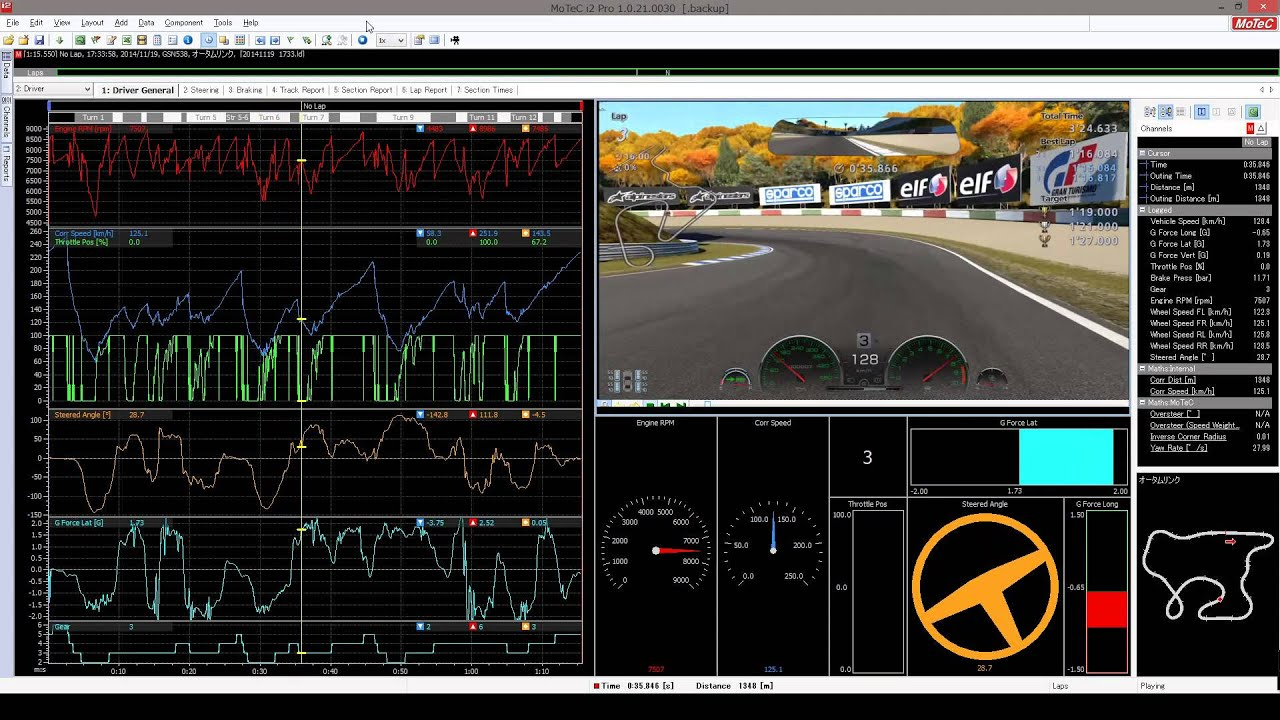
\includegraphics[width=0.6\linewidth]{./figs/herramientas/analisis/motec.png}
	\caption[Captura de Motec i2 Pro]{Captura de Motec i2 Pro \cite{motec_cap}}
    \label{fig:motec}
\end{figure}

\subsection{Mu}
Mu \cite{mu} es un exportador de telemetría que convierte los archivos de telemetría de iRacing (.ibt) en archivos que pueden ser leídos por el software i2 de MoTeC para su análisis. Entre sus características destacan la capacidad de exportar en formatos MoTeC y \ac{csv}, la exportación en unidades métricas o imperiales, y la activación automática de la captura de telemetría en iRacing. Además, Mu guarda una copia de la configuración utilizada para generar la telemetría y ofrece una interfaz de usuario que puede ejecutarse en segundo plano.

\subsection{McLaren Atlas}
McLaren Atlas \cite{atlas} es una herramienta de telemetría avanzada utilizada en competiciones de alto nivel como la Fórmula 1. Diseñada para proporcionar análisis detallados del rendimiento del vehículo (\autoref{fig:atlas}), Atlas permite a los ingenieros y pilotos comprender mejor el comportamiento del coche y optimizar su rendimiento. Sus características incluyen la capacidad de manejar grandes volúmenes de datos, realizar análisis detallados de cada componente del vehículo y generar informes claros que facilitan la interpretación de los datos y la implementación de mejoras específicas basadas en dichos análisis.

\begin{figure}[H]
	\centering
	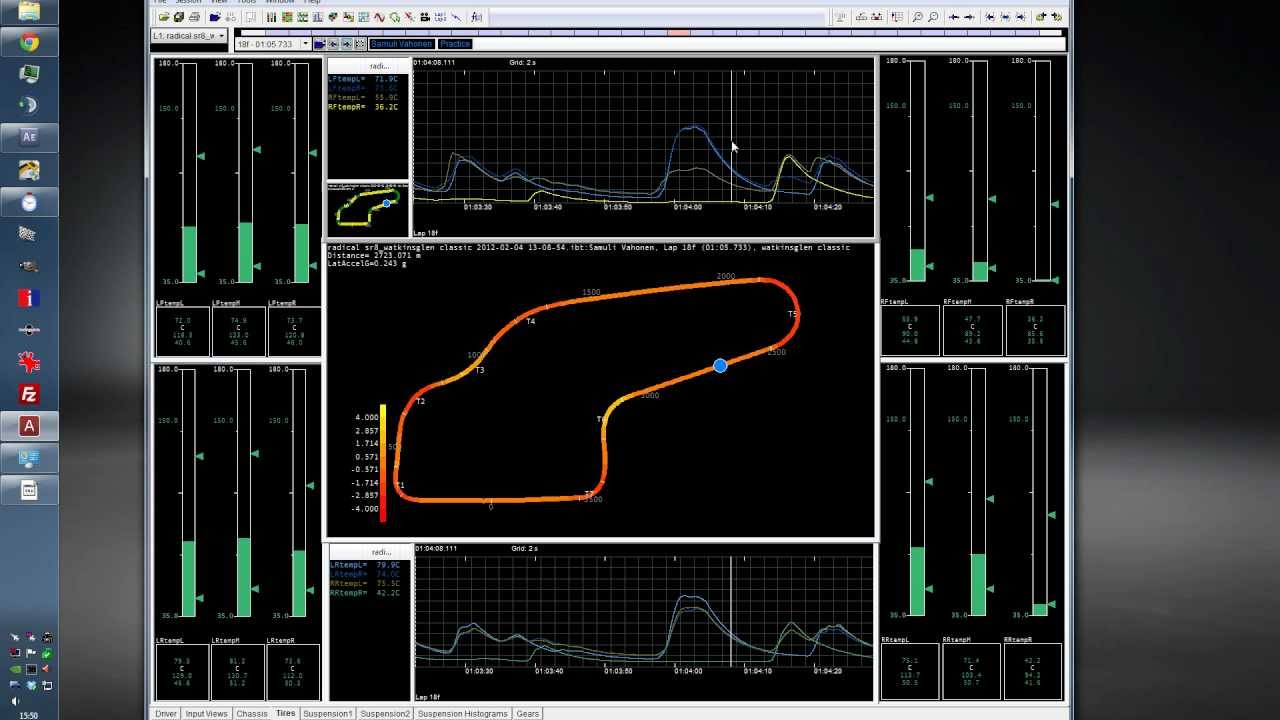
\includegraphics[width=0.6\linewidth]{./figs/herramientas/analisis/mclaren_atlas.png}
	\caption[Captura de McLaren Atlas]{Captura de McLaren Atlas \cite{atlas_cap}}
    \label{fig:atlas}
\end{figure}

\subsection{Sim Racing Telemetry}
Sim Racing Telemetry \cite{srt} es una herramienta versátil diseñada para el análisis de datos de telemetría en Simracing. Ofrece una interfaz amigable que permite a los usuarios importar datos de diversas plataformas de simulación y analizarlos mediante gráficos interactivos y comparaciones de vueltas (\autoref{fig:srt}). Entre sus características principales se incluyen la capacidad de comparar datos de múltiples sesiones, visualizar métricas clave en tiempo real y generar informes detallados. Esta herramienta es ideal tanto para aficionados como para profesionales que buscan mejorar su rendimiento en las simulaciones de carreras.
\begin{figure}[H]
	\centering
	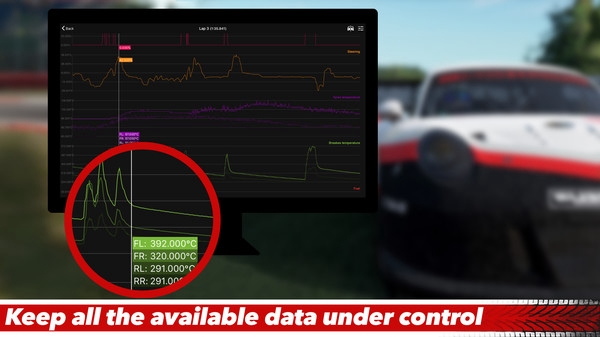
\includegraphics[width=0.6\linewidth]{./figs/herramientas/analisis/simracingtelemetry.png}
	\caption[Imagen promocional de Sim Racing Telemetry]{Imagen promocional de Sim Racing Telemetry \cite{srt_cap}}
    \label{fig:srt}
\end{figure}

\section{Entrenadores virtuales de Simracing}
En el Simracing, los entrenadores virtuales han revolucionado la forma en que los pilotos mejoran sus habilidades y estrategias de carrera. Estas herramientas proporcionan análisis detallados, asesoría personalizada y recursos educativos para ayudar a los simracers a alcanzar su máximo potencial. Esta sección explora algunos de los entrenadores virtuales más destacados, detallando sus características principales y cómo pueden beneficiar a los pilotos en su búsqueda de excelencia en las pistas virtuales.

\subsection{Virtual Racing School}
\ac{vrs} \cite{vrs} es una plataforma integral de entrenamiento que ofrece análisis de telemetría, tutoriales en vídeo, sesiones de entrenamiento en vivo con pilotos profesionales y programas de desarrollo personalizados. \ac{vrs} permite a los usuarios comparar sus datos con los de los mejores pilotos, identificar áreas de mejora y aplicar estrategias para optimizar su rendimiento en pista (\autoref{fig:vrs}). Además, proporciona recursos educativos a través de su academia en línea y soporte continuo para sus usuarios.
\begin{figure}[H]
	\centering
	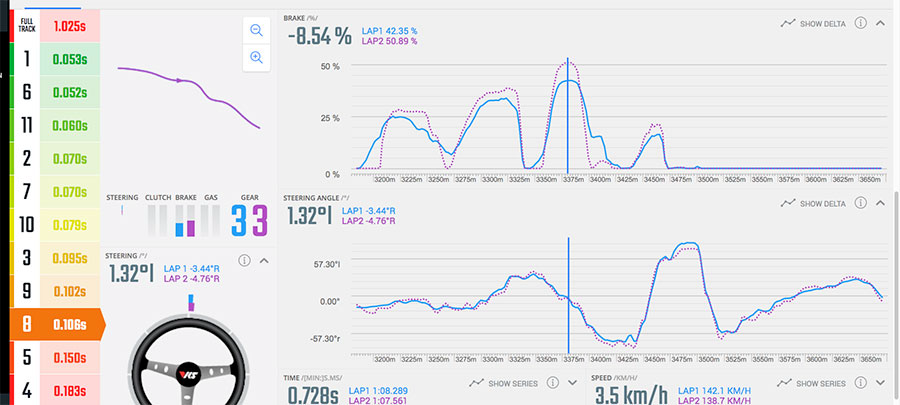
\includegraphics[width=0.6\linewidth]{./figs/herramientas/mentor_virtual/vrs.png}
	\caption[Imagen promocional de \ac{vrs}]{Imagen promocional de \ac{vrs} \cite{vrs_cap}}
    \label{fig:vrs}
\end{figure}

\subsection{Garage 61}
Garage 61 \cite{g61} es un servicio de mentoría personalizado para Simracers que se enfoca en el análisis detallado de telemetría, sesiones de práctica guiadas y retroalimentación en tiempo real (\autoref{fig:g61}). Las principales características de Garage 61 incluyen la adaptación de los programas de entrenamiento a las necesidades específicas de cada piloto y el acceso a un equipo de expertos en Simracing que ofrecen asesoramiento continuo. Esta plataforma ayuda a los pilotos a mejorar sus habilidades mediante un enfoque estructurado y personalizado.
\begin{figure}[H]
	\centering
	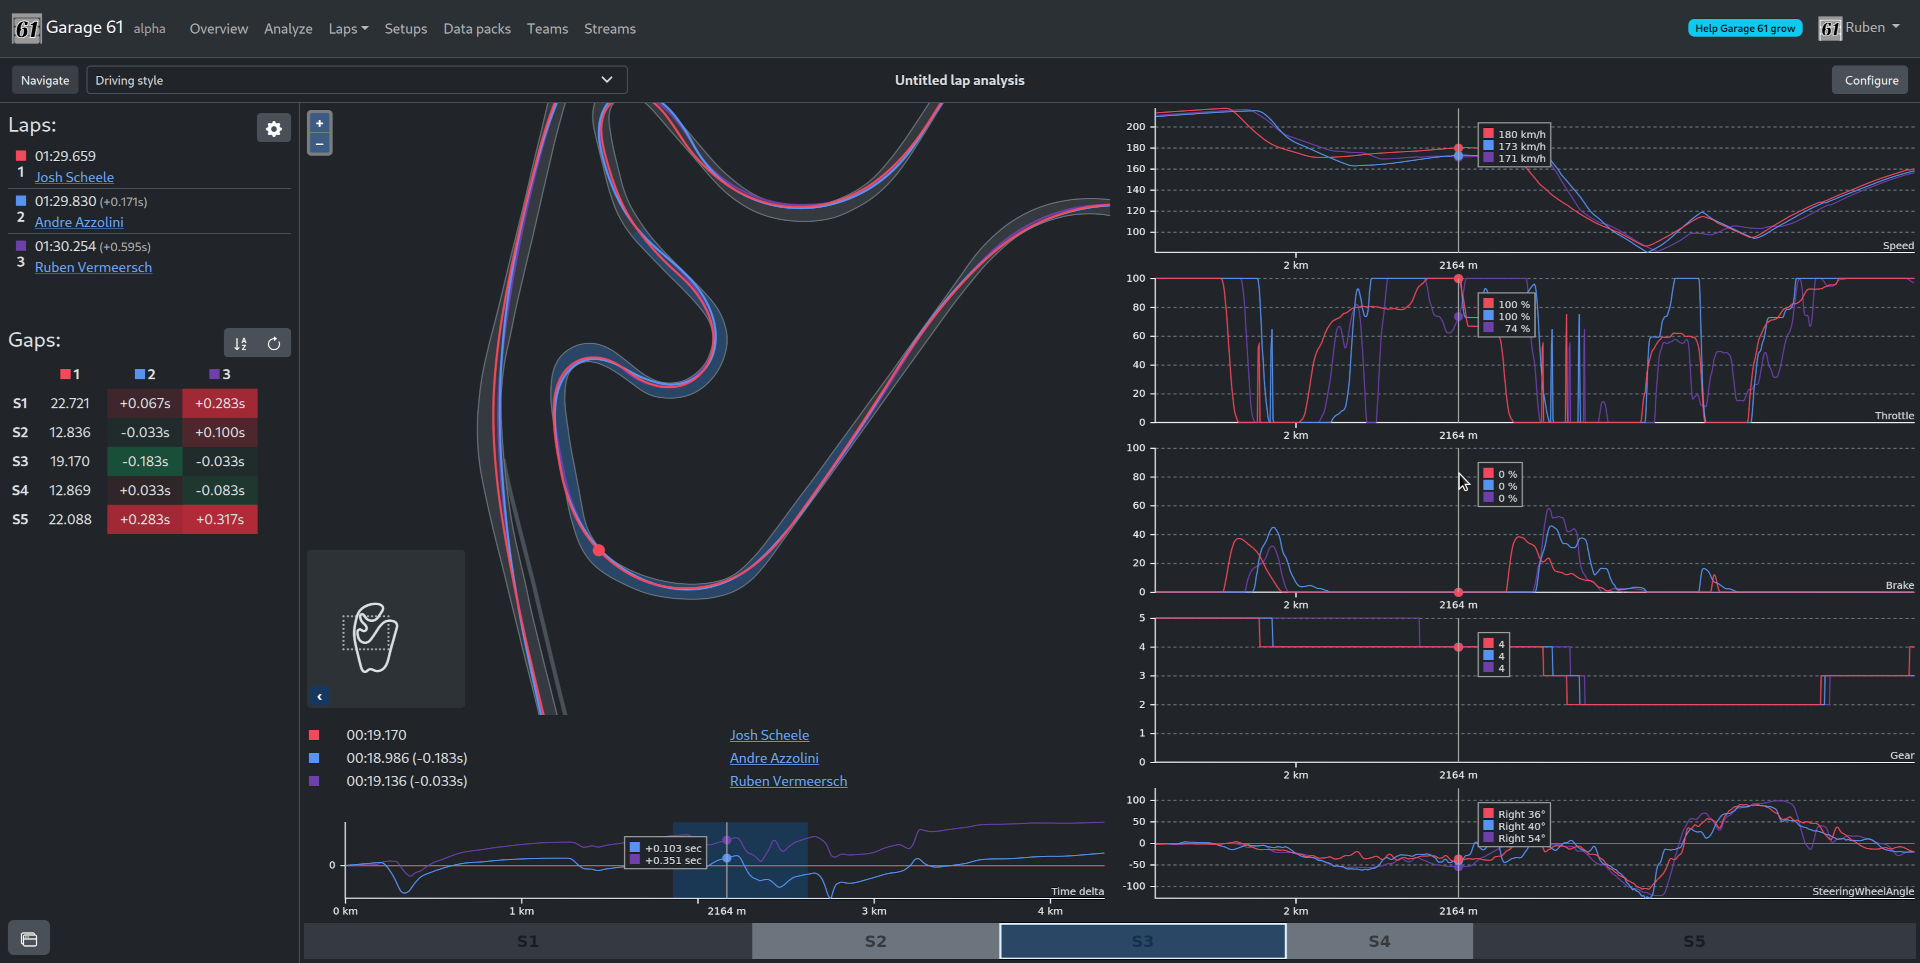
\includegraphics[width=0.6\linewidth]{./figs/herramientas/mentor_virtual/garage61.png}
	\caption[Imagen promocional de Garage 61]{Imagen promocional de Garage 61 \cite{g61_cap}}
    \label{fig:g61}
\end{figure}

\subsection{Grid-and-go Virtual Coach}
Grid-and-go Virtual Coach \cite{gg_vc} es una herramienta de mentoría en línea diseñada para mejorar el rendimiento de los Simracers mediante el análisis de datos y la asesoría personalizada (\autoref{fig:ggvc}). Ofrece una interfaz intuitiva para el análisis de telemetría, programas de entrenamiento estructurados y consejos estratégicos para la carrera. Entre sus características destacadas se encuentran la capacidad de establecer metas de rendimiento personalizadas, recibir recomendaciones basadas en datos y acceder a una comunidad de pilotos para compartir experiencias y estrategias.
\begin{figure}[H]
	\centering
	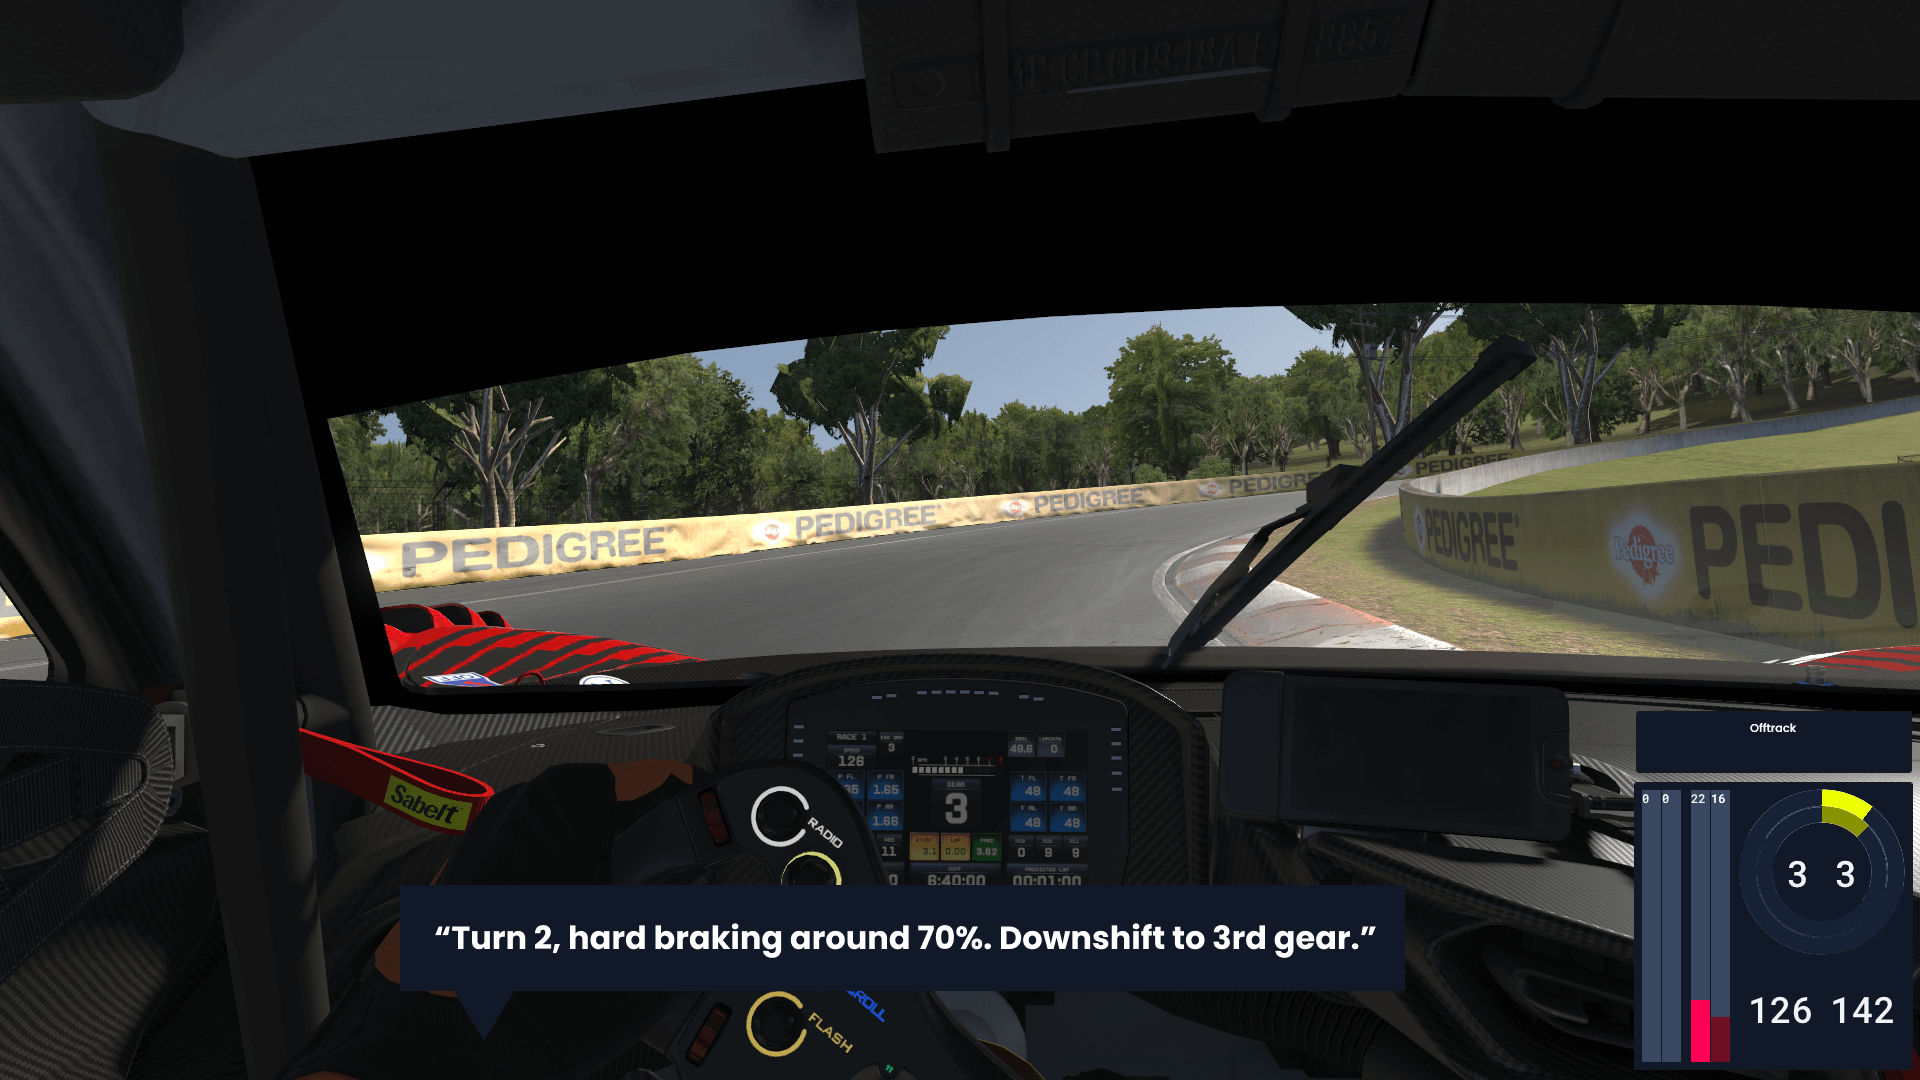
\includegraphics[width=0.6\linewidth]{./figs/herramientas/mentor_virtual/gg_virtual_coach.png}
	\caption[Imagen promocional de Grid-and-go Virtual Coach]{Imagen promocional de Grid-and-go Virtual Coach \cite{gg_vc_cap}}
    \label{fig:ggvc}
\end{figure}

\section{Repositorios abiertos de herramientas}
En el ámbito del Simracing, los repositorios abiertos de herramientas proporcionan a los desarrolladores y entusiastas la capacidad de personalizar y mejorar sus experiencias de simulación mediante el acceso a software y bibliotecas de código abierto. Estos recursos permiten la creación de aplicaciones avanzadas y la integración de funcionalidades adicionales que enriquecen el análisis y la práctica del Simracing. A continuación, se describen algunos de los repositorios más relevantes disponibles para la comunidad de Simracing.

\subsection{iRSDK}
iRSDK \cite{irsdk} es un clon del SDK oficial de iRacing en C++. Este repositorio proporciona una API limpia y ampliada que reemplaza la API de telemetría original de iRacing, soportando múltiples clientes y ofreciendo una lista expandida de funciones. iRSDK permite el acceso a datos de telemetría en tiempo real y la grabación de datos en disco, facilitando el desarrollo de aplicaciones que interactúan con la telemetría de iRacing para análisis y monitoreo en vivo.

\subsection{pyirsdk}
pyirsdk \cite{pyirsdk} es una implementación en Python 3 del SDK de iRacing. Este repositorio permite obtener datos de la sesión (como información del evento y de la sesión) y datos de telemetría en vivo, como velocidad y nivel de combustible. Además, soporta el envío de mensajes de difusión para controlar la cámara, reproducir repeticiones y ejecutar comandos durante el juego o mientras se permanece en el área de pit, zona de servicio y mantenimiento del vehículo. pyirsdk facilita la integración de la telemetría de iRacing en aplicaciones Python, proporcionando una herramienta poderosa y flexible para el análisis y el desarrollo en Simracing.

\subsection{itelem}
itelem \cite{itelem} es una herramienta de análisis de telemetría que convierte los archivos de telemetría de iRacing (.ibt) en un formato que puede ser utilizado para análisis detallado. Este repositorio permite a los usuarios desarrollar aplicaciones personalizadas para procesar y visualizar datos de telemetría, facilitando el estudio de diversos aspectos del rendimiento del vehículo y del piloto. Su diseño modular permite extensiones y adaptaciones según las necesidades específicas de los usuarios.

\subsection{ibt-telemetry}
ibt-telemetry \cite{ibt-telemetry} es una biblioteca destinada a la manipulación y análisis de archivos de telemetría .ibt de iRacing. Esta herramienta permite leer y procesar los datos almacenados en los archivos de telemetría, facilitando el desarrollo de aplicaciones que requieren acceso a información detallada de las sesiones de conducción. Con ibt-telemetry, los desarrolladores pueden extraer y analizar datos específicos para mejorar el rendimiento y la comprensión del comportamiento del vehículo en diferentes condiciones de carrera.

\section{Aprendizaje no supervisado}
El uso del aprendizaje automático, y en particular del aprendizaje no supervisado, ha demostrado ser fundamental en el análisis de datos complejos, como los que se generan en la telemetría de Simracing. Las técnicas de aprendizaje no supervisado, como el agrupamiento, permiten identificar patrones y asociar automáticamente datos similares sin necesidad de etiquetado previo \cite{Jain1988, Duda2000}. Esto es especialmente útil para categorizar vectores de diferencias en las variables de telemetría, facilitando la interpretación y el análisis de grandes volúmenes de datos. Al agrupar las diferencias en categorías significativas, estas técnicas proporcionan una visión más clara del rendimiento y comportamiento del vehículo y del piloto, permitiendo la optimización de estrategias de conducción basadas en datos precisos y categorizados\cite{Hastie2009, Bishop2006}.

\subsection{K-Means}
El algoritmo K-means es una técnica de aprendizaje no supervisado ampliamente utilizada para la agrupación de datos (\autoref{fig:km}). En el contexto del análisis de telemetría en Simracing, K-means es particularmente útil para categorizar las diferencias en las variables de telemetría, debido a su capacidad para minimizar la variabilidad dentro de los grupos y maximizar las diferencias entre ellos \cite{MacQueen1967}. Este proceso permite identificar patrones subyacentes en los datos de telemetría, facilitando la comprensión de las áreas donde se pueden realizar mejoras.

Una de las ventajas clave de utilizar K-means es que las categorías generadas tienden a estar ordenadas de manera natural. Esto significa que las diferencias en las variables de telemetría pueden agruparse en categorías jerárquicas, como ''muy poca diferencia negativa'', ''diferencia negativa'', ''igual'', ''diferencia positiva'' y ''mucha diferencia positiva''. Este ordenamiento facilita la asignación de etiquetas en lenguaje natural, lo que hace que los resultados sean fácilmente interpretables por los usuarios \cite{Jain1988, Hartigan1979}. Al proporcionar una descripción clara y ordenada de las diferencias, los pilotos pueden entender rápidamente las áreas que requieren atención y las acciones específicas que deben tomar para mejorar su rendimiento.

\begin{figure}[H]
	\centering
	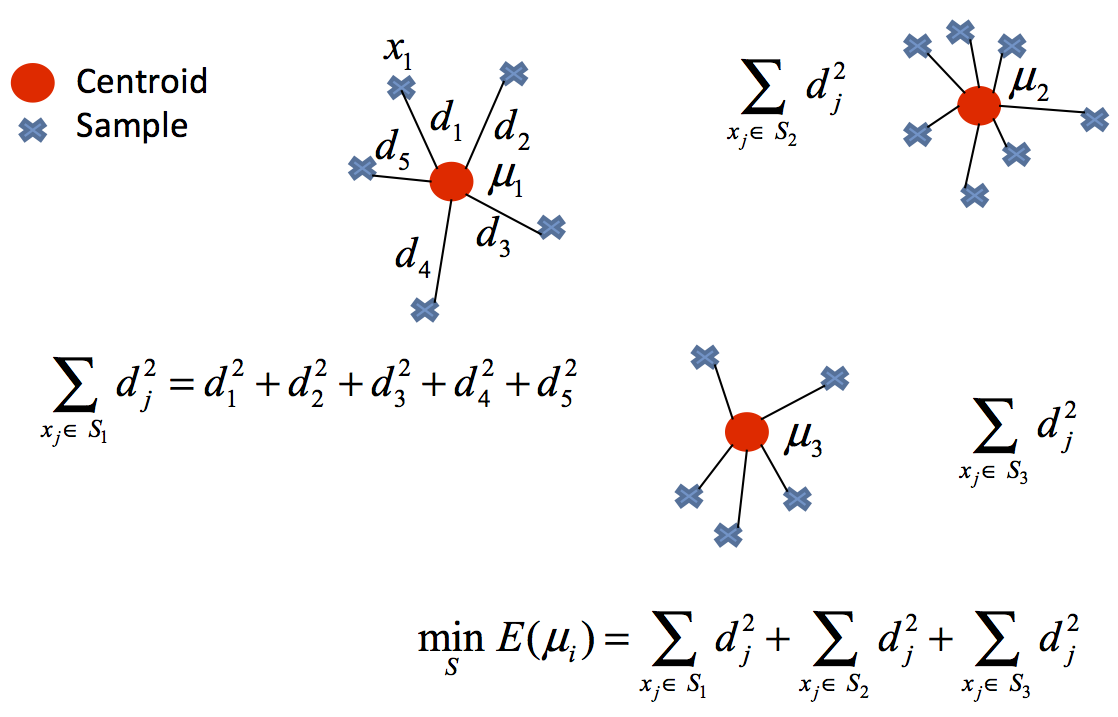
\includegraphics[width=0.6\linewidth]{./figs/aprendizaje_no_supervisado/k_means.png}
	\caption[Ilustración K-means (K = 3)]{Ilustración K-means (K = 3) \cite{UniOviedoKMeans}}
    \label{fig:km}
\end{figure}

\subsection{Fuzzy C-Means}

\ac{fcm} es un algoritmo de agrupamiento que permite que un punto de datos pertenezca a múltiples agrupaciones con diferentes grados de pertenencia (\autoref{fig:fcm}), en lugar de asignar cada punto a una sola agrupación de manera rígida. Esto se logra minimizando una función de costo que considera tanto la distancia entre los puntos de datos y los centroides de las agrupaciones como los grados de pertenencia \cite{Bezdek1981, Hathaway1996, Dunn1973, Pal1995}.

\begin{figure}[H]
	\centering
	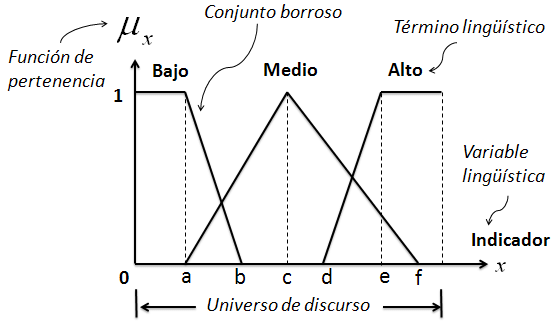
\includegraphics[width=0.6\linewidth]{./figs/aprendizaje_no_supervisado/conjuntos_borrosos.png}
	\caption[Ejemplo de conjuntos borrosos]{Ejemplo de conjuntos borrosos \cite{ResearchGateFuzzySets}}
    \label{fig:fcm}
\end{figure}

El algoritmo \ac{fcm} ofrece una mayor flexibilidad y precisión en la categorización de datos de telemetría en Simracing al permitir que cada punto de datos pertenezca a múltiples agrupaciones con diferentes grados de pertenencia. Esto facilita una interpretación más detallada y matizada, especialmente en presencia de ruido y ambigüedad en los datos. Los grados de pertenencia ayudan a generar etiquetas lingüísticas más comprensibles y graduales, mejorando la comprensión de los resultados. \ac{fcm} también es más adaptable a diferentes escenarios y condiciones cambiantes, proporcionando una herramienta versátil para el análisis de datos.
\chapter{Plan de gestión del trabajo}\label{cap:Planificacion}
Este capítulo detalla todos los aspectos relacionados con la gestión del proyecto para la creación de un entrenador virtual de Simracing. Abarca desde la metodología de desarrollo seleccionada hasta las tecnologías y recursos necesarios, pasando por la gestión de la configuración y aseguramiento de la calidad, la planificación del trabajo y la estimación de costes y análisis de riesgos. El objetivo es proporcionar una estructura clara y predecible que permita un desarrollo eficiente y de alta calidad, asegurando así que el entrenador virtual pueda ofrecer recomendaciones precisas y útiles basadas en datos de telemetría.


\section{Metodología de Desarrollo}
En esta sección se abordaron dos enfoques fundamentales utilizados en el proyecto: \ac{xp} como metodología de gestión de proyectos y \ac{ddd} como metodología de desarrollo de software. \ac{xp} fue aplicada para gestionar el proyecto de manera ágil, facilitando la comunicación continua y la adaptación rápida a los cambios. Por otro lado, \ac{ddd} se empleó para estructurar y organizar el código del software, enfocándose en modelar las reglas y procesos del dominio del problema de manera precisa y coherente. Ambas metodologías, al ser integradas, contribuyeron significativamente al éxito y la calidad del proyecto.


\subsection{Extreme Programming \textit{(\ac{xp})}}
\ac{xp} es una metodología ágil de desarrollo de proyectos software, aunque en la actualidad se ha extrapolado a otros campos, que se centra en mejorar la calidad del software y la capacidad de respuesta a los cambios en los requisitos del cliente. \ac{xp} es conocido por su enfoque en la comunicación, la simplicidad, la retroalimentación, valores que son fundamentales para su aplicación efectiva \cite{Beck2004}. En este proyecto, se ha adoptado \ac{xp} debido a su capacidad para manejar cambios constantes y su énfasis en la entrega continua de valor al cliente.

\begin{figure}[H]
	\centering
	
\includegraphics[width=0.4\linewidth]{./figs/herramientas/desarrollo/extreme_programming.png}
	\caption[Diagrama \ac{xp}]{Diagrama \ac{xp} \cite{xp_wiki}}
\end{figure}

\subsubsection*{Implementación de \ac{xp} en el Proyecto}
\label{sec:impl_xp}
En este proyecto, se han identificado y definido tres roles principales: desarrollador, consultor y cliente. Estos roles han sido desempeñados por el autor del proyecto, un usuario experto en Simracing y los directores del trabajo, respectivamente.

\begin{itemize}[noitemsep]
\item \textbf{Desarrollador}: Responsable de la implementación y codificación del proyecto, siguiendo las prácticas de \ac{xp}.
\item \textbf{Consultor}: Proporciona asesoramiento técnico y orientación sobre aspectos específicos del proyecto.
\item \textbf{Clientes}: Actúan como directores del trabajo, proporcionando retroalimentación continua y estableciendo las prioridades y requisitos del proyecto.
\end{itemize}

En cuanto a la estructuración del trabajo, éste se dividió en sprints semanales, siguiendo un modelo similar al de Scrum, que es compatible con los principios de \ac{xp}. Cada lunes a las 17:00 se mantuvo una reunión que englobaba tanto la revisión del sprint como su planificación. Durante estas reuniones, se presentaron los avances realizados, se evaluaron los resultados y se propusieron cambios. Además, se priorizaba el backlog de tareas para la siguiente semana.

Estas reuniones semanales permitieron una serie de iteraciones y prototipos, ajustándose continuamente a la visión de los clientes y garantizando que cada entrega incrementase el valor del proyecto. Este enfoque iterativo y adaptativo es un componente clave de \ac{xp}, el cual ha asegurado que el desarrollo se alinee estrechamente con las necesidades de los clientes y ha permitido realizar ajustes rápidos en respuesta a los comentarios recibidos.

\subsubsection*{Gestión del Proyecto con GitHub Projects}
La gestión del proyecto se ha llevado a cabo mediante GitHub Projects, donde se estructuraron las tareas e hitos. Inicialmente, se estableció un hito para cada sub-objetivo del proyecto (\autoref{fig:ghp_milestones}). A medida que el proyecto avanzó, se crearon nuevas tareas dentro del hito correspondiente según las necesidades emergentes del mismo.
\begin{figure}[H]
	\centering
	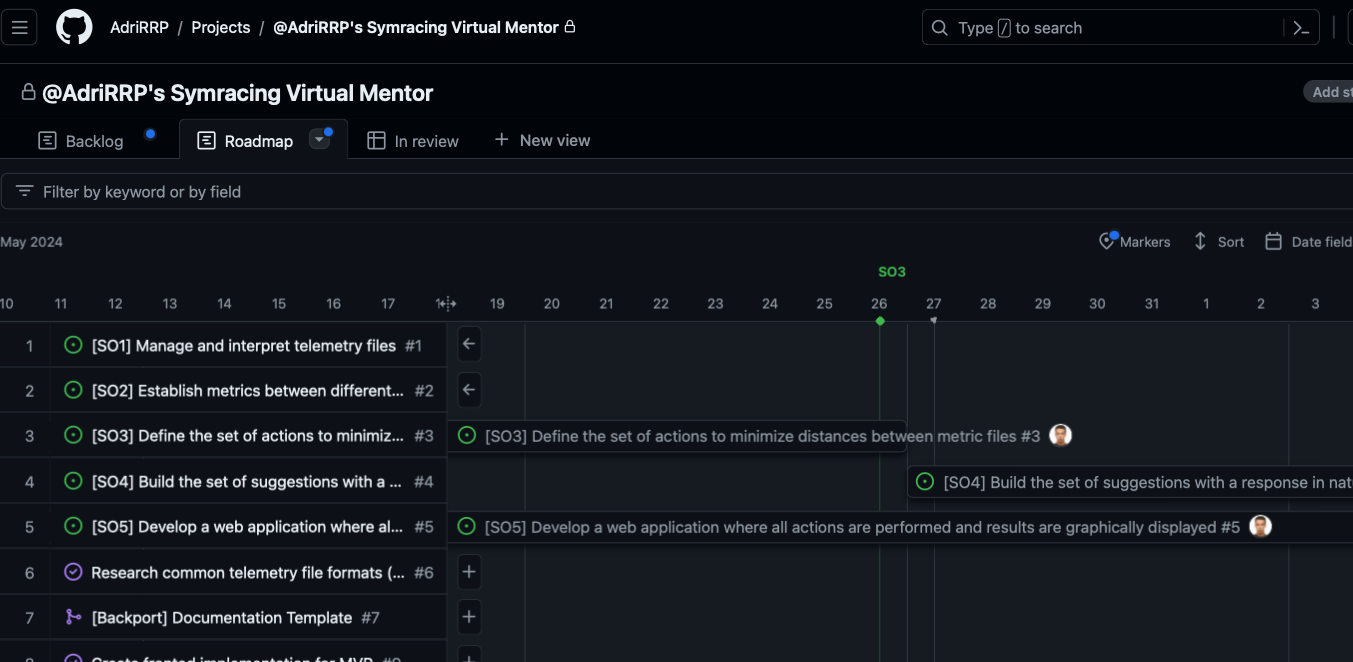
\includegraphics[width=0.8\linewidth]{./figs/herramientas/desarrollo/ghproject_roadmap.png}
	\caption[Captura de roadmap de GitHub Projects]{Captura de roadmap de GitHub Projects}
 \label{fig:ghp_milestones}
\end{figure}


El uso del tablero de tareas en GitHub Projects ha sido una herramienta fundamental en la gestión ágil de este proyecto, proporcionó una visualización clara y estructurada del flujo de trabajo además de facilitar la colaboración y el seguimiento del progreso. El tablero de GitHub Projects se organizó en cinco paneles distintos: ''milestones'' (hitos), ''backlog'' (lista de tareas pendientes), ''in progress'' (en curso), ''ready'' (listas para ser ejecutadas) y ''done'' (finalizadas) (\autoref{fig:ghp_board}).

\begin{figure}[H]
	\centering
	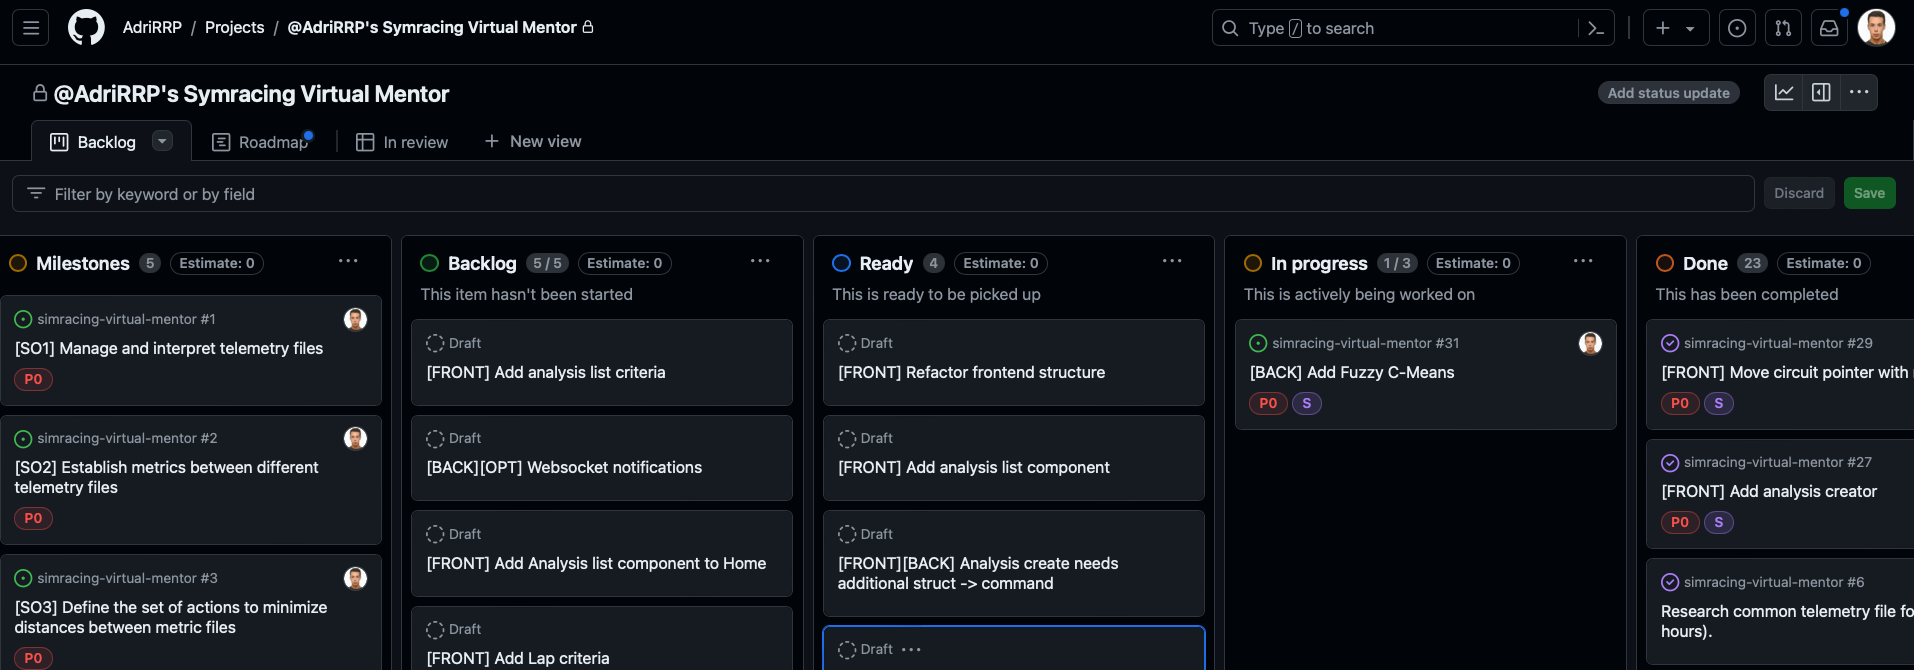
\includegraphics[width=0.9\linewidth]{./figs/herramientas/desarrollo/ghproject_board.png}
	\caption[Captura de tablero de GitHub Projects]{Captura de tablero de GitHub Projects}
    \label{fig:ghp_board}
\end{figure}

\begin{itemize}[noitemsep]
\item El panel \textbf{''milestones''} permitió a los miembros del equipo visualizar el progreso de los hitos de un vistazo, asegurando que los objetivos a largo plazo se  mantenían en el horizonte y se alineaban con las expectativas del cliente.
\item El panel \textbf{''backlog''} contenía todas las tareas necesarias para completar los hitos, proporcionando un depósito centralizado de trabajo pendiente que se gestionó y priorizó continuamente.
\item El panel \textbf{''ready''} indicaba qué tareas estaban listas para ser abordadas tras haber pasado por el proceso de refinamiento y priorización.
\item El panel \textbf{''in progress''} mostraba las tareas que estaban desarrollándose, permitiendo al equipo y a los interesados ver qué trabajo se estaba llevando a cabo en tiempo real.
\item El panel \textbf{''done''} contenía las tareas completadas, ofreciendo una visión clara de lo que ya se había logrado y ayudando a medir el progreso de los objetivos establecidos.\\
\end{itemize}

Desde GitHub Projects también se gestionaron las incidencias. Cada incidencia se daba de alta con un título y una descripción, además se le asignaba un estado inicial de borrador (draft). Durante las reuniones de planificación del sprint, en las que se revisaba el progreso y se establecían nuevos objetivos con el cliente, se examinaban estas incidencias o se creaban nuevas. Se les asignaba una prioridad (etiquetadas como P0, P1 o P2) para indicar su urgencia. Además, cada incidencia recibía una talla, un concepto similar a los puntos de esfuerzo de Scrum que cuantifica el esfuerzo requerido, utilizando una escala similar a los tamaños de ropa, que va desde XS hasta XL (\autoref{fig:ghp_issue}). Posteriormente, la incidencia se movía al backlog para que el programador pudiera asignársela.

\begin{figure}[H]
	\centering
	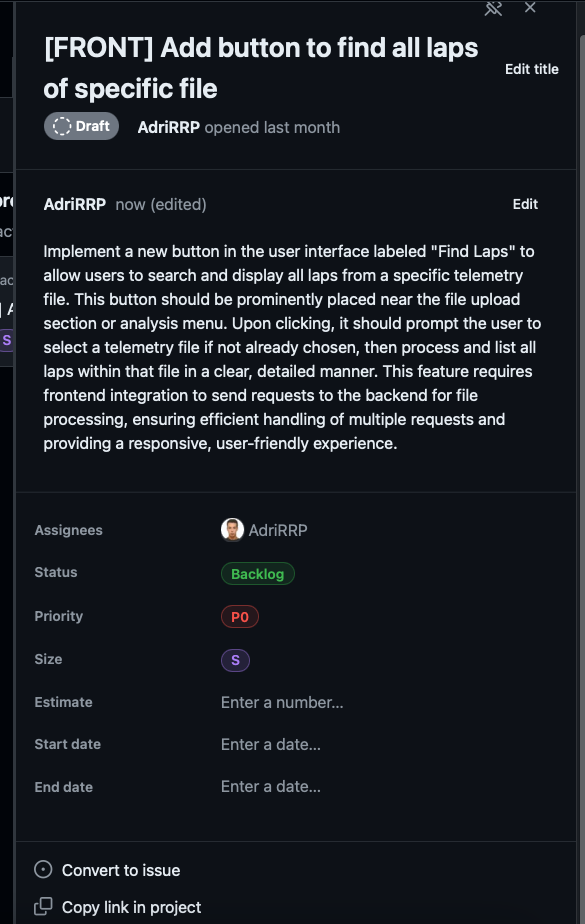
\includegraphics[width=0.30\linewidth]{./figs/herramientas/desarrollo/ghproject_issue.png}
	\caption[Captura de incidencia de GitHub Projects]{Captura de incidencia de GitHub Projects}
    \label{fig:ghp_issue}
\end{figure}

\subsection{Domain Driven Design \textit{(\ac{ddd}}) y Arquitectura Hexagonal}
La adopción de \ac{ddd} y la Arquitectura Hexagonal en este proyecto fue una decisión estratégica que permitió manejar la complejidad y asegurar la flexibilidad y escalabilidad del entrenador virtual de Simracing.

\begin{itemize}[noitemsep]
\item \textbf{Domain-Driven Design}: \ac{ddd} se centra en construir un modelo de dominio que refleje con precisión los conceptos y reglas del dominio específico del negocio. En este proyecto, se ha aplicado \ac{ddd} para estructurar las capas de dominio y aplicación de manera efectiva, asegurando que la lógica de negocio esté bien definida y separada de las preocupaciones técnicas. Esto permite una mejor alineación con los requisitos del cliente y facilita la colaboración entre desarrolladores y expertos en el dominio \cite{Evans2004}. La estructura de directorios del proyecto refleja esta separación, con módulos claramente definidos para diferentes partes del dominio, como \textit{ibt\_extractor, analysis, file y lap}.
\item \textbf{Arquitectura Hexagonal}: La Arquitectura Hexagonal, propuesta por Alistair Cockburn, busca desacoplar el núcleo de la aplicación de las interfaces externas (\autoref{fig:hex_arch}), permitiendo que el sistema sea más adaptable a cambios futuros y facilitando la integración con nuevas tecnologías \cite{Cockburn2005}. En este proyecto, la arquitectura hexagonal se ha implementado mediante la separación de los componentes de la aplicación en capas bien definidas, con directorios dedicados a infraestructura, aplicación, y dominio. Esto no sólo ha mejorado la mantenibilidad del código, sino que también ha permitido realizar pruebas más efectivas y gestionar la complejidad de manera más eficiente.
\end{itemize}

\begin{figure}[H]
	\centering
	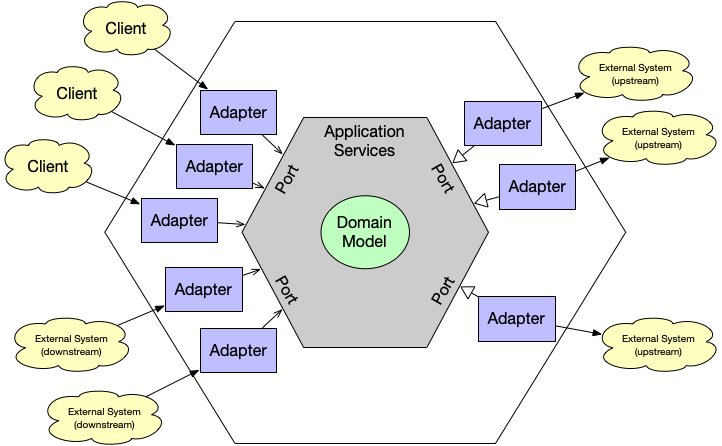
\includegraphics[width=0.5\linewidth]{./figs/herramientas/desarrollo/hexagonal.png}
	\caption[Esquema de Arquitectura Hexagonal]{Esquema de Arquitectura Hexagonal \cite{hexagonal_architecture}}
    \label{fig:hex_arch}
\end{figure}

La combinación de \ac{ddd} y la Arquitectura Hexagonal en este proyecto ha permitido desarrollar un sistema modular y escalable, con un backend robusto basado en principios de diseño estratégico y táctico. El uso de eventos y suscriptores en el backend, junto con la implementación de controladores y repositorios, ha asegurado que la lógica de negocio esté desacoplada de las interfaces técnicas, facilitando la evolución del sistema según las necesidades de los clientes.

\section{Recursos}
En esta sección se detallan los recursos que han sido necesarios para la realización del proyecto, clasificados en hardware, software y humanos, éstos últimos revisados en la sección \hyperref[sec:impl_xp]{metodología de desarrollo}. Además, se incluye una estimación del coste total del proyecto basada en estos recursos. Este análisis ha permitido una comprensión clara de las inversiones requeridas y de cómo se han distribuido los esfuerzos, así como las herramientas empleadas para el desarrollo del asistente virtual de Simracing.

\subsection{Recursos Hardware}
En esta sección se describen los recursos hardware utilizados durante  el desarrollo del proyecto. Este análisis incluye tanto los componentes principales del hardware como sus características relevantes.

\begin{itemize}
\item MacBook Pro M2 (Apple M2 Pro, 16GB RAM, 1TB SSD, monitor Liquid Retina XDR 14 pulgadas).
\item 2 Monitores Phillips Brilliance 241B (24 pulgadas, Full HD).
\item Ratón MSI Interceptor DS300 (7.200 DPI, ergonómico).
\item Teclado Razer Huntsman (mecánico, retroiluminado).
\item Estación de anclado StarTech DK30A2DHU (USB-C, dual HDMI).
\item Router TP-Link Archer AX50.
\end{itemize}

\begin{figure}[H]
	\centering
	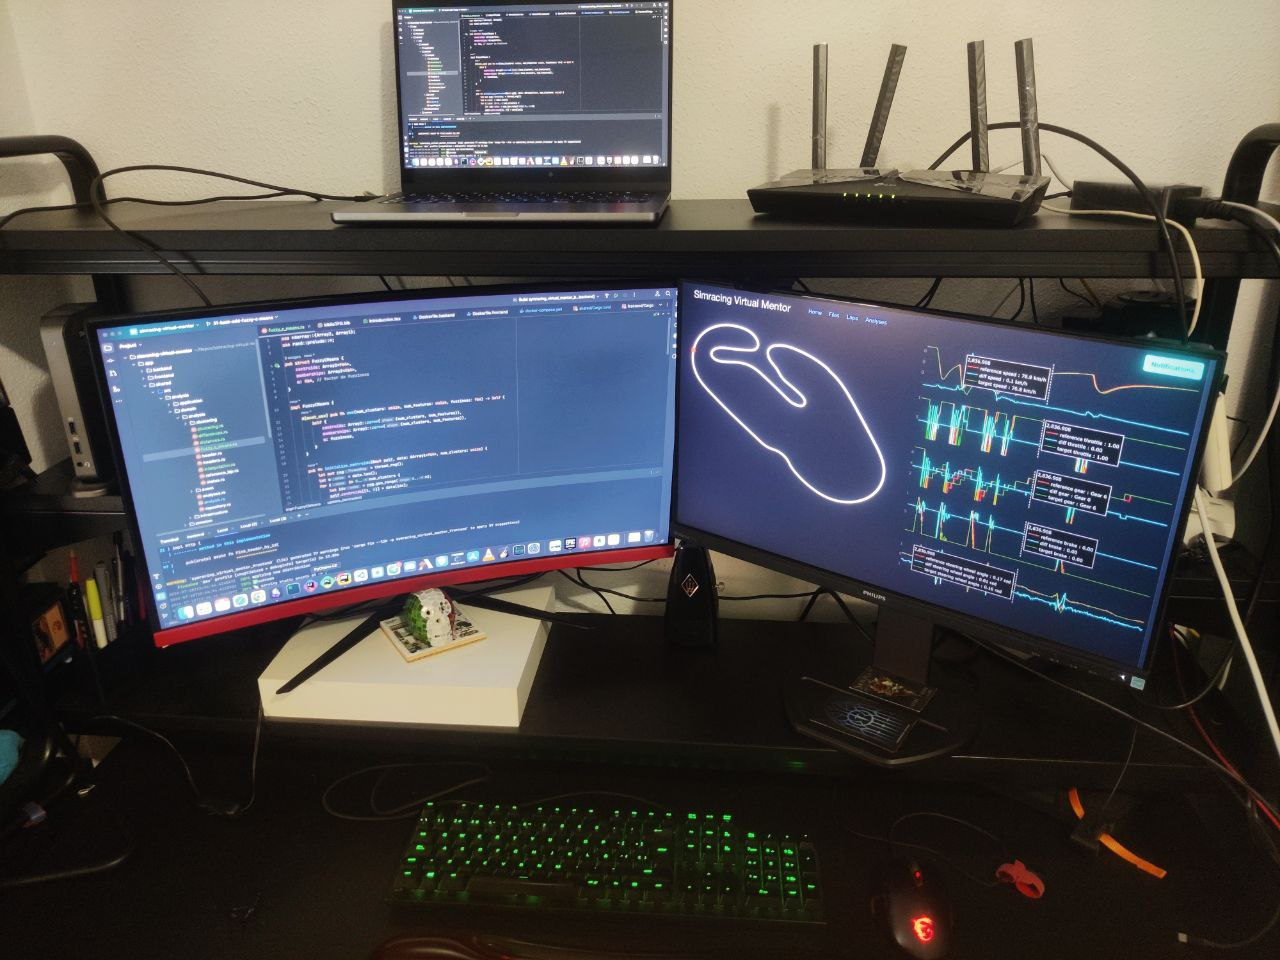
\includegraphics[width=0.70\linewidth]{./figs/herramientas/hardware/recursos_hardware.png}
	\caption[Recursos Hardware utilizados]{Recursos Hardware utilizados}
    \label{fig:recursos_hardware}
\end{figure}


\subsection{Recursos Software}
\subsubsection*{Sistemas Operativos}
\begin{itemize}
\item macOS Sonoma 14.5 (23F79) \cite{macos14_5_release_notes}
\end{itemize}

\subsubsection*{Lenguajes}
\begin{itemize}
\item Programación
    \begin{itemize}
    \item \textbf{Rust 1.79.0}: Lenguaje de programación que enfatiza seguridad, concurrencia y eficiencia, ideal para desarrollar aplicaciones de alto rendimiento sin comprometer la robustez \cite{rust_release_notes_1_79}.
    \end{itemize}
\item Scripting
    \begin{itemize}
    \item \textbf{JavaScript}: Lenguaje de programación interpretado que se utiliza para el desarrollo de aplicaciones web dinámicas y la manipulación del \ac{dom} \cite{mozilla_js}.
    \item \textbf{Dockerfile Syntax}: Lenguaje de configuración utilizado para definir entornos y aplicaciones Docker mediante instrucciones y comandos específicos en un archivo de texto estructurado \cite{dockerfile}.
    \item \textbf{Bash}: Lenguaje de scripting utilizado en sistemas Unix para automatización de tareas y gestión de comandos \cite{bash}.
    \end{itemize}
\item Marcado
    \begin{itemize}
    \item \textbf{\ac{html}}: Lenguaje de marcado  estándar para crear y estructurar páginas web \cite{html}.
    \item \textbf{\ac{json}}: Formato ligero de intercambio de datos fácil de leer y escribir \cite{json}.
    \item \textbf{\ac{yaml}}: Formato de serialización de datos legible por humanos que se utiliza principalmente para archivos de configuración \cite{yaml}.
    \item \textbf{\ac{toml}}: Lenguaje de marcado diseñado para la configuración, enfocándose en la simplicidad y legibilidad humana \cite{toml}.
    \end{itemize}
\item Estilo
    \begin{itemize}
    \item \textbf{\ac{css}}: Lenguaje de estilo usado para describir la presentación de un documento \ac{html} \cite{rust_release_notes_1_79}.
    \end{itemize}
\end{itemize}
\subsubsection*{Bases de Datos}
\begin{itemize}
\item \textbf{MongoDB 7.0} Base de datos NoSQL orientada a documentos \cite{mongodb}.
\item \textbf{MongoDB Compass 1.43.1}: interfaz gráfica para MongoDB que permite explorar, analizar y manipular los datos \cite{mongodb_compass}.
\end{itemize}

\subsubsection*{Librerías}
\begin{itemize}
\item Rust
    \begin{itemize}
    \item \textbf{async-trait 0.1.80}: Permite definir y utilizar traits asíncronos en Rust \cite{async_trait}.
    \item \textbf{axum 0.7.5}: Framework para construir aplicaciones web en Rust con soporte para Tokio \cite{axum}.
    \item \textbf{base64 0.22.1}: Librería para la codificación y decodificación de datos en Base64 \cite{base64}.
    \item \textbf{bson 2.11.0}: Implementación de BSON para Rust, utilizada para trabajar con MongoDB \cite{bson}.
    \item \textbf{chrono 0.4.38}: Librería para la manipulación y formateo de fechas y tiempos \cite{chrono}.
    \item \textbf{config 0.14.0}: Proporciona soporte para la configuración basada en archivos y entornos \cite{config}.
    \item \textbf{futures 0.3.30}: Librería para la programación asíncrona y manejo de futuros en Rust \cite{futures}.
    \item \textbf{futures-util 0.3.30}: Utilidades adicionales para trabajar con futuros en Rust \cite{futures_util}.
    \item \textbf{gloo 0.11.0}: Conjunto de utilidades para el desarrollo de aplicaciones web en Rust \cite{gloo}.
    \item \textbf{gloo-events 0.1}: Librería para trabajar con eventos en aplicaciones web \cite{gloo_events}.
    \item \textbf{gloo-net 0.5.0}: Librería para realizar solicitudes de red en aplicaciones web \cite{gloo_net}.
    \item \textbf{js-sys 0.3.69}: Enlaza cada \ac{api} del sistema JavaScript con Rust \cite{js_sys}.
    \item \textbf{log 0.4.21}: Proporciona una interfaz de registro de logs para Rust \cite{log}.
    \item \textbf{mime 0.3.17}: Librería para trabajar con tipos MIME \cite{mime}.
    \item \textbf{mockall 0.12.1}: Herramienta para crear mocks en Rust durante las pruebas \cite{mockall}.
    \item \textbf{mongodb 2.8.2}: Cliente oficial de MongoDB para Rust \cite{mongodb_crate}.
    \item \textbf{ndarray 0.15.6}: Librería para el manejo de arreglos multidimensionales en Rust \cite{ndarray}.
    \item \textbf{plotly 0.8.4}: Librería para crear gráficos interactivos en Rust \cite{plotly}.
    \item \textbf{rand 0.8.5}: Librería para la generación de números aleatorios \cite{rand}.
    \item \textbf{reqwest 0.12.4}: Cliente \ac{http} simple y eficaz para Rust \cite{reqwest}.
    \item \textbf{serde 1.0.203}: Librería de serialización y deserialización en Rust \cite{serde}.
    \item \textbf{serde-json 1.0.117}: Extensión de Serde para trabajar con JSON \cite{serde_json}.
    \item \textbf{serde-wasm-bindgen 0.6.5}: Librería para la serialización y deserialización con wasm-bindgen \cite{serde_wasm_bindgen}.
    \item \textbf{serde-yaml 0.9}: Extensión de Serde para trabajar con YAML \cite{serde_yaml}.
    \item \textbf{sha256 1.5.0}: Librería para calcular hashes SHA-256 \cite{sha256}.
    \item \textbf{thiserror 1.0.61}: Proporciona una manera ergonómica de definir errores \cite{thiserror}.
    \item \textbf{tokio 1.38.0}: Runtime asíncrono para Rust con soporte para I/O y timers \cite{tokio}.
    \item \textbf{tower-http 0.5.2}: Conjunto de utilidades y middleware para trabajar con servicios \ac{http} \cite{tower_http}.
    \item \textbf{tracing 0.1.40}: Librería para instrumentar aplicaciones Rust para el registro de logs estructurados \cite{tracing}.
    \item \textbf{tracing-subscriber 0.3.18}: Colección de suscriptores para manejar la salida de tracing \cite{tracing_subscriber}.
    \item \textbf{urlencoding 2.1.3}: Librería para la codificación y decodificación de URLs \cite{urlencoding}.
    \item \textbf{uuid 1.8.0}: Librería para la generación y manejo de \ac{uuid} \cite{uuid}.
    \item \textbf{wasm-bindgen 0.2.92}: Proporciona soporte para la interoperabilidad entre Rust y WebAssembly \cite{wasm_bindgen}.
    \item \textbf{wasm-bindgen-futures 0.4.42}: Extensión de wasm-bindgen para trabajar con futuros \cite{wasm_bindgen_futures}.
    \item \textbf{wasm-bindgen-file-reader 1.0.0}: Librería para la lectura de archivos en aplicaciones WebAssembly \cite{wasm_bindgen_file_reader}.
    \item \textbf{wasm-logger 0.2.0}: Implementación de un logger para aplicaciones WebAssembly \cite{wasm_logger}.
    \item \textbf{web-sys 0.3.69}: Enlaza las \ac{api}s del sistema Web con Rust \cite{web_sys}.
    \item \textbf{yew 0.21}: Framework para el desarrollo de aplicaciones web con WebAssembly \cite{yew}.
    \item \textbf{yew-hooks 0.3.2}: Conjunto de hooks para el framework Yew \cite{yew_hooks}.
    \item \textbf{yew-router 0.18.0}: Librería para el enrutamiento en aplicaciones Yew \cite{yew_router}.
    \end{itemize}
\item JavaScript
    \begin{itemize}
    \item \textbf{Plotly JS 2.33.0}: Librería de gráficos interactivos \cite{plotly_js}.
    \end{itemize}
\item \ac{css}
    \begin{itemize}
    \item \textbf{Bulma 1.0.0}: Framework \ac{css} moderno y adaptable. 
    \end{itemize}
\end{itemize}

\subsubsection*{Herramientas de construcción}
\begin{itemize}
\item \textbf{Cargo 1.79.0}: Gestor de paquetes Rust \cite{rust_cargo}.
\item \textbf{Trunk 0.20.2}: Herramienta para construir y desplegar aplicaciones Web basadas en WebAssembly para Rust \cite{trunk}.
\item \textbf{xx 1.4.0}: Herramienta de compilación cruzada y multi-plataforma \cite{xx}.
\end{itemize}

\subsubsection*{Herramientas de desarrollo}
\begin{itemize}
\item \textbf{RustRover 2024.1}: Entorno de desarrollo para Rust \cite{rust_rover}.
\item \textbf{Vim 9.0}: Editor de texto avanzado \cite{vim}.
\item \textbf{xxd 1.4.0}: Herramienta para visualizar datos en hexadecimal \cite{xxd}.
\item \textbf{Google Chrome 126.0.6478.127}: Navegador web desarrollado por Google \cite{chrome}.
\end{itemize}

\subsubsection*{Documentación}
\begin{itemize}
\item \textbf{\LaTeX}: Sistema de preparación de documentos que utiliza macros y formato TEX \cite{latex_project}.
\item \textbf{Overleaf}: Plataforma colaborativa para redacción científica en LaTeX \cite{overleaf}.
\item \textbf{ChatGPT 4o}: Modelo de lenguaje desarrollado por OpenAI utilizado para asistir en la redacción, estructuración y documentación del contenido de este proyecto \cite{chatgpt}.
\end{itemize}

\subsection{Coste}
En esta sección se realiza una estimación de los costes totales del proyecto, teniendo en cuenta los recursos hardware y humanos necesarios. El software utilizado es de carácter libre, por lo que no se incluye en la estimación de costes. A continuación se presentan los detalles y cálculos:
\begin{itemize}
    \item \textbf{Costes de recursos humanos:}
    \begin{itemize}
    \item Desarrollador Rust (nivel medio): 200 horas.
    \item Gerentes (clientes/directores del trabajo): 20 horas cada uno.
    \item Consultor experto en Simracing: 8 horas.
    \end{itemize}

    \item Según los datos del mercado laboral en España \cite{randstad,glassdoor,kiwiremoto}:
    \begin{itemize}
    \item Salario medio de un desarrollador Rust nivel medio: 25 €/hora.
    \item Salario medio de un gerente: 35 €/hora.
    \item Salario medio de un consultor: 45 €/hora.
    \end{itemize}

    \item \textbf{Costes de recursos hardware:}
    \begin{itemize}
    \item MacBook Pro M2 Pro de 14 pulgadas: 2.400 €.
    \item 2 Monitores Phillips Brilliance 241B: 400 € (200 € cada uno).
    \item Ratón MSI Interceptor DS300: 50 €.
    \item Teclado Razer Huntsman: 150 €.
    \item Estación de anclado StarTech DK30A2DHU: 200 €.
    \item Router TP-Link Archer AX50: 150 €.
    \end{itemize}

    \item \textbf{Cálculo de costes:}
    \begin{itemize}
    \item Coste del desarrollador: 200 horas * 25 €/hora = 5.000 €.
    \item Coste de los gerentes: 2 * 20 horas * 35 €/hora = 1.400 €.
    \item Coste del consultor: 8 horas * 45 €/hora = 360 €.
    \item Coste total del hardware: 2.400 € + 400 € + 50 € + 150 € + 200 € + 150 € = 3.350 €.
    \end{itemize}
\end{itemize}

\begin{table}[H]
\centering
\begin{tabular}{|l|c|}
\hline
\textbf{Recurso} & \textbf{Coste (€)} \\ \hline
Desarrollador (200 horas a 25 €/hora) & 5.000 \\ \hline
Gerentes (2 personas, 20 horas cada una a 35 €/hora) & 1.400 \\ \hline
Consultor (8 horas a 45 €/hora) & 360 \\ \hline
MacBook Pro M2 Pro de 14 pulgadas & 2.400 \\ \hline
2 Monitores Phillips Brilliance 241B & 400 \\ \hline
Ratón MSI Interceptor DS300 & 50 \\ \hline
Teclado Razer Huntsman & 150 \\ \hline
Estación de anclado StarTech DK30A2DHU & 200 \\ \hline
Router TP-Link Archer AX50 & 150 \\ \hline
Electricidad (uso proporcional: 20\% de 6 meses a 50 €/mes) & 60 \\ \hline
Internet (uso proporcional: 50\% de 6 meses a 30 €/mes) & 90 \\ \hline
\textbf{Total} & \textbf{10.260} \\ \hline
\end{tabular}
\caption{Coste total del proyecto desglosado por recursos}
\label{tab:costes_proyecto}
\end{table}

\section{Aseguramiento de la Calidad}
El aseguramiento de la calidad en este proyecto fue gestionado de manera integral utilizando varias estrategias y herramientas clave. A continuación se describe cómo se aplicaron estas medidas.

\subsection{Pruebas}
Rust ofrece un robusto sistema de testing integrado que se utilizó para realizar las pruebas del entrenador virtual de Simracing.
Se utilizó el enfoque de \ac{ddd} para estructurar el proyecto de manera que la lógica de negocio estuviera bien definida y aislada. Esto facilitó la creación de \textbf{pruebas unitarias} para el dominio de la aplicación.
Las \textbf{pruebas de integración} verificaron la coherencia y el correcto funcionamiento de los diferentes servicios (casos de uso/historias de usuario) sin necesidad de disponer de la infraestructura (repositorios y servicios externos) y por tanto sin acoplarse a ella. Esto fue posible gracias a \ac{ddd} y la separación entre las capas de aplicación e infraestructura.


\subsection{Análisis y Formato de Código}
Para mantener un formato de código estándar y mejorar la calidad del mismo, se utilizaron las herramientas \textbf{Cargo fmt} y \textbf{Clippy}. Cargo fmt aseguró que todo el código siguiera las convenciones de estilo de Rust, mejorando la legibilidad y facilitando la colaboración entre desarrolladores. Clippy se utilizó para realizar análisis estáticos del código, identificando posibles errores, malas prácticas y sugiriendo mejoras.


\subsection{Flujo de \ac{cicd} con GitHub Actions}
Se estableció un flujo de integración y entrega continua \ac{cicd} utilizando GitHub Actions \cite{github_actions}. Este flujo automatizado aseguraba que todos las pruebas se ejecutaran antes de integrar cambios en la rama principal (main). El proceso de \ac{cicd} incluía controles de calidad que utilizaban Codecov \cite{codecov} para medir la cobertura de los tests y garantizar que se mantenían altos estándares de calidad.

Los tres archivos clave en la carpeta `.github/workflows` fueron:
\begin{itemize}
    \item \textbf{clippy.yaml}: Configuración para ejecutar clippy y asegurar que el código seguía las mejores prácticas.
    \item \textbf{coverage.yaml}: Configuración para medir la cobertura de los tests con Codecov.
    \item \textbf{tests.yaml}: Configuración para ejecutar todos los tests unitarios e integrados del proyecto.
\end{itemize}

Estas prácticas permitieron identificar y corregir errores de manera temprana y aseguraron que el código cumpliera consistentemente con los estándares de calidad definidos. El uso de estas herramientas y metodologías no sólo mejoró la calidad del software, sino que también facilitó un desarrollo más ágil y eficiente.

\section{Riesgos}
Al inicio del proyecto de desarrollo del entrenador virtual para Simracing, se identificaron y evaluaron varios riesgos potenciales que podrían afectar el éxito del mismo. Estos riesgos se abordaron con un enfoque sistemático para mitigar su impacto y garantizar un desarrollo fluido.

\begin{itemize}
    \item Uno de los riesgos principales identificados fue la \textbf{complejidad técnica del proyecto}. La implementación de \ac{ddd} y la Arquitectura hexagonal implicaba un nivel elevado de abstracción y modularidad que requería una comprensión profunda de estos conceptos por parte del desarrollador. Esto se mitigó mediante el estudio y la aplicación gradual de estas metodologías, así como con la consultoría especializada de un experto en Simracing.
    \item Otro riesgo significativo fue la \textbf{integración de tecnologías y herramientas diversas}. La utilización de Rust como lenguaje principal, junto con MongoDB para la gestión de datos, y herramientas como GitHub Actions para \ac{cicd}, requería una integración cuidadosa y coordinada. Para mitigar este riesgo, se definieron claramente las responsabilidades de cada componente del sistema y se implementaron pruebas unitarias e integradas para asegurar la correcta interoperabilidad.
    \item Además, la \textbf{gestión de la calidad del código} se identificó como un riesgo crucial. La utilización de Clippy y Cargo fmt fue esencial para mantener un estándar de codificación elevado y consistente. Sin embargo, se reconoció que la configuración de estas herramientas podría ser desafiante y consumir tiempo. Este riesgo se manejó configurando Clippy con sus vertientes más restrictivas desde el inicio y asegurando que el desarrollador se familiarizara con su uso.
    \item Finalmente, el riesgo asociado al \textbf{despliegue y mantenimiento del sistema} se abordó mediante la implementación de un flujo de \ac{cicd} robusto utilizando GitHub Actions y Codecov. Este enfoque permitió una integración continua y un despliegue controlado, minimizando los errores y asegurando una cobertura de pruebas adecuada antes de cualquier fusión en la rama principal del proyecto.
\end{itemize}

En resumen, la identificación y gestión proactiva de estos riesgos fue fundamental para el éxito del proyecto, permitiendo abordar desafíos técnicos complejos y asegurar un alto nivel de calidad en el desarrollo del entrenador virtual para Simracing.
\chapter{Resultados}
\label{cap:Resultados}

En este capítulo, se detalla el proceso de creación del entrenador virtual de Simracing, abarcando todas las etapas del proyecto desde la concepción hasta su implementación final. La primera sección de este capítulo detalla cómo se comenzó el proyecto, y cada sección sucesiva representa un hito correspondiente a cada objetivo específico del proyecto, de acuerdo a lo expuesto en el \autoref{cap:Objetivo}. Dentro de cada hito, se desglosan las historias de usuario llevadas a cabo para cumplir dichos objetivos específicos. Esta estructura permite una visión clara y organizada de cómo se desarrolló el proyecto, mostrando de manera precisa cómo se abordaron y resolvieron los distintos desafíos técnicos y de implementación para alcanzar los objetivos establecidos.

\section{Inicio y preparación}
Esta sección detalla los pasos iniciales y preparativos necesarios para el desarrollo del proyecto.

Una vez aprobado el proyecto, se llevó a cabo una reunión inicial con los clientes para establecer los preparativos necesarios. En esta reunión, se discutió el alcance del proyecto, se definieron las tecnologías y lenguajes de programación a utilizar, y se introdujeron los requisitos preliminares para el desarrollo del entrenador virtual de Simracing.

Se decidió utilizar Rust debido a sus ventajas en rendimiento y seguridad de memoria, esenciales para el procesamiento eficiente de datos de telemetría. Rust fue utilizado para desarrollar tanto el backend como el frontend, con el objetivo de facilitar la reutilización del \textit{Shared Kernel} de \ac{ddd} y garantizar la coherencia en la lógica de negocio entre ambos componentes. Además, se planificó la integración de \ac{wasm} en la parte del frontend para permitir una ejecución rápida y eficiente en el navegador (\autoref{fig:rust_wasm}), proporcionando una experiencia de usuario fluida y cumpliendo con las demandas de aplicaciones intensivas en cálculos y procesamiento de datos.

\begin{figure}[H]
	\centering
	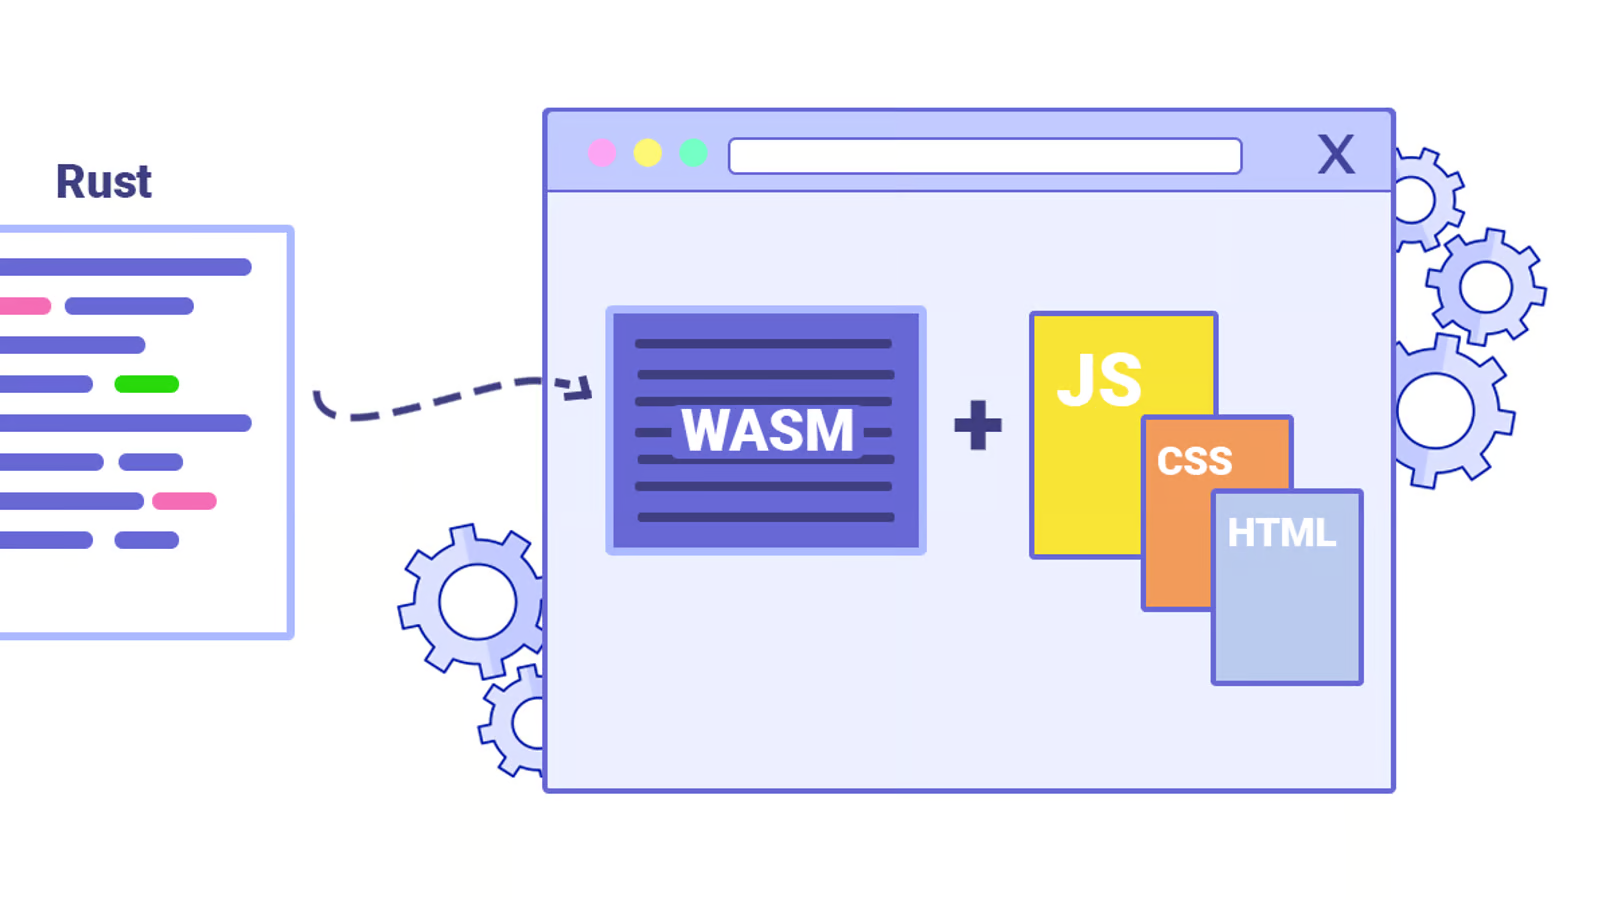
\includegraphics[width=0.7\linewidth]{./figs/herramientas/desarrollo/wasm_rust.png}
	\caption[Interacción Rust-WebAssembly]{Interacción Rust-WebAssembly \cite{garg2023}}
    \label{fig:rust_wasm}
\end{figure}

Durante la planificación inicial del proyecto, se introdujeron los conceptos básicos del Simracing al programador para asegurar una comprensión adecuada del contexto y las necesidades del proyecto. Posteriormente, se sostuvo una reunión de acercamiento con el consultor, quien, además de competir en un equipo de Simracing, posee conocimiento y experiencia en la creación de software específico para este ámbito. En esta reunión, se discutieron elementos técnicos relevantes del Simracing, incluyendo las plataformas competitivas, los diferentes tipos de análisis, en tiempo real o a posteriori, y las herramientas existentes.

Adicionalmente, se creó el repositorio inicial en GitHub (\autoref{fig:estructura_inicial_de_directorios}) y se registró el proyecto en GitHub Projects. En esta plataforma se añadieron los objetivos preliminarmente acordados y se configuraron tanto el software como las cuentas necesarias para el desarrollo del proyecto. Este enfoque sistemático aseguró una base sólida para el desarrollo del entrenador virtual, facilitando la coordinación y la gestión eficiente del proyecto desde sus etapas iniciales.

\begin{figure}[H]
    \centering
    \begin{forest}
        for tree={
            font=\ttfamily,
            grow'=0,
            child anchor=west,
            parent anchor=south,
            anchor=west,
            calign=first,
            edge path={
                \noexpand\path [draw, \forestoption{edge}]
                (!u.parent anchor) |- (.child anchor)\forestoption{edge label};
            },
            inner sep=1pt,
            l sep=10pt,
            fit=band,
            before typesetting nodes={
                if n=1
                {insert before={[,phantom]}}
                {}
            },
            where level=0{line width=1pt}{},
            before computing xy={l=20pt},
        }
        [raíz/
            [app/ , label={right:\footnotesize (Código fuente de la aplicación completa)}
                [backend/, label={right:\footnotesize (Código fuente del backend)}]
                [frontend/, label={right:\footnotesize (Código fuente del frontend)}]
                [shared/, label={right:\footnotesize (Código fuente compartido, \textit{Shared Kernel} en \ac{ddd})}]
            ]
            [docs/, label={right:\footnotesize (Documentación del proyecto)}
                [drafts/, label={right:\footnotesize (Borradores con información relevante)}]
                [report/, label={right:\footnotesize (Código fuente \LaTeX de este documento)}]
            ]
            [.gitignore, label={right:\footnotesize (Definición de los ficheros que no forman parte del proyecto)}]
            [LICENSE, label={right:\footnotesize (Definición de la licencia del proyecto)}]
            [README.md, label={right:\footnotesize (Documentación técnica sobre qué es el proyecto y cómo usarlo)}]
        ]
    \end{forest}
    \caption{Estructura inicial de directorios}
    \label{fig:estructura_inicial_de_directorios}
\end{figure}

\section{Hito 1: Adquisición y procesamiento de datos de telemetría \textit{(SO1)}}
Esta hito abarcó las actividades relacionadas con la adquisición y procesamiento de datos de telemetría, esenciales para el desarrollo del entrenador virtual de Simracing. Se investigaron los formatos de ficheros de telemetría más comunes, se desarrolló un módulo para la carga de estos ficheros y se implementaron algoritmos para la extracción e interpretación de información relevante. La validación de los datos extraídos se realizó mediante su presentación en formato tabular, asegurando la integridad y usabilidad de la información procesada. En la \autoref{tab:resumen_hito_1} se muestra un resumen del primer hito. Se debe recordar que los sprints son semanales por le que este hito abarcaría de las semanas 1 a la 9. 

\begin{table}[H]
\centering
\begin{tabular}{|l|c|}
\hline
\textbf{Título} & Adquisición y procesamiento de datos de telemetría \\ \hline
\textbf{Código} & \textit{SO1} \\ \hline
\textbf{Historias de Usuario} & 4 \\ \hline
\textbf{Sprints} & 1-9 \\ \hline
\end{tabular}
\caption{Resumen del Hito 1}
\label{tab:resumen_hito_1}
\label{tab
}
\end{table}

A continuación, se detallarán las historias de usuario desarrolladas para la adquisición y procesamiento de datos de telemetría, especificando sus objetivos, prioridades y tiempos de implementación.

\subsection{Investigación de los formatos más utilizados en ficheros de telemetría}
\begin{table}[H]
\centering
\begin{tabular}{|l|p{10cm}|}
\hline
\multicolumn{2}{|c|}{\textbf{Historia de Usuario 1}} \\ \hline
\textbf{Nombre:} & Investigar formatos comunes de ficheros de telemetría \\ \hline
\textbf{Descripción:} & Como cliente del proyecto, quiero que se identifiquen y evalúen los formatos de ficheros de telemetría más utilizados en la industria del Simracing, para seleccionar el más adecuado para este proyecto. \\ \hline
\textbf{Prioridad:} & P1 \\ \hline
\textbf{Talla:} & S \\ \hline
\textbf{Sprints:} & 1 \\ \hline
\end{tabular}
\caption{Historia de Usuario 1}
\label{tab:us_telemetria}
\end{table}

En el proceso de investigación para determinar los formatos de ficheros de telemetría más utilizados en la industria del Simracing, se realizó un análisis exhaustivo de las opciones disponibles. Se descubrió que la gran mayoría de simuladores expone sus datos de telemetría en formatos específicos, que pueden ser transformados en formatos tabulares para facilitar su análisis a posteriori.

\subsubsection*{Principales Formatos de Telemetría}
\begin{itemize}
    \item \textbf{Formato \ac{ibt}}: El formato .ibt es utilizado por iRacing para almacenar datos de telemetría. Estos ficheros contienen una gran cantidad de información detallada sobre las carreras, incluyendo datos de velocidad, revoluciones por minuto, posición en la pista, entre otros. Este formato es binario y se utiliza principalmente para análisis a posteriori, donde los datos se pueden convertir a formatos tabulares como \ac{csv} para facilitar su procesamiento y análisis.

    \item \textbf{Formato Motec}: Motec es otro formato comúnmente utilizado en simuladores como rFactor y Project CARS. Los datos de telemetría se almacenan en archivos binarios que pueden ser leídos por el software Motec, permitiendo un análisis detallado de las sesiones de carrera. Al igual que el formato \ac{ibt}, los datos pueden ser exportados a formatos tabulares para la realización de un  análisis más intuitivo.
    
    \item \textbf{Formato \ac{acti}}: Assetto Corsa utiliza el formato \ac{acti} para exponer datos de telemetría. Este formato permite la recolección de datos detallados sobre el rendimiento del vehículo y el comportamiento en pista. Los datos de \ac{acti} también pueden ser convertidos a formatos tabulares.
\end{itemize}

\subsubsection*{Análisis en Tiempo Real vs. Análisis a Posteriori}

Durante la investigación, se distinguió entre los análisis en tiempo real y los análisis a posteriori:

\begin{itemize}
    \item \textbf{Análisis en Tiempo Real}: Utiliza el \ac{sdk} proporcionado por los desarrolladores de juegos que permiten acceder a datos de telemetría en tiempo real. Estos \ac{sdk}s son esenciales para aplicaciones que requieren actualizaciones instantáneas, como paneles de control en vivo y herramientas de monitorización durante las carreras. Ejemplos incluyen el \ac{sdk} de iRacing y la \ac{api} de Telemetría de Assetto Corsa.
    \item \textbf{Análisis a Posteriori}: Este tipo de análisis se realiza una vez finalizada la sesión de simulación. Los datos de telemetría se guardan en formatos binarios como \ac{ibt} y Motec y luego se convierten a tablas para su análisis detallado. Existen diversas herramientas específicas para realizar esta conversión y facilitar el análisis.
\end{itemize}

\subsubsection*{Uso de \ac{ibt} de iRacing}
Se justificó el uso del formato \ac{ibt} de iRacing en el proyecto debido a las siguientes razones:

\begin{itemize}
    \item \textbf{Compatibilidad y Popularidad}: El formato \ac{ibt} es ampliamente utilizado en la comunidad de iRacing, garantizando una gran cantidad de recursos y herramientas disponibles para su análisis.
    \item \textbf{Detalle y Precisión}: Proporciona datos de telemetría extremadamente detallados y precisos, esenciales para realizar análisis profundos que mejoren el rendimiento del usuario en el simulador.
    \item \textbf{Integración con Herramientas Existentes}: Numerosas herramientas y librerías soportan el formato \ac{ibt}, lo que facilita su integración en el flujo de trabajo del proyecto y permite aprovechar las capacidades de análisis avanzadas que estas herramientas ofrecen.
    \item \textbf{Futuro análisis en tiempo real}: Aunque podrían haberse utilizado datos tabulares directamente, se eligió el formato \ac{ibt} para permitir futuros análisis en tiempo real. En la propuesta del proyecto, se destacó esta opción como potencialmente interesante para mejorar la flexibilidad y alcance del análisis de datos en Simracing.
\end{itemize}

\subsubsection*{Adquisición de Ficheros de Telemetría}

Para obtener los ficheros \ac{ibt} de telemetría es necesario tener una suscripción de pago a iRacing, además de contar con un equipo hardware de elevado coste para la conducción. La colaboración del consultor fue crucial en este contexto. No solo nos guió en la investigación, sino que también nos proporcionó un fichero de telemetría de un entrenamiento, permitiéndonos avanzar ágilmente en los siguientes pasos del proyecto. Su intervención subrayó la importancia de contar con un experto en la materia para optimizar procesos y asegurar la calidad del desarrollo.


\subsection{Desarrollar un módulo para la carga de ficheros de telemetría}
\begin{table}[H]
\centering
\begin{tabular}{|l|p{10cm}|}
\hline
\multicolumn{2}{|c|}{\textbf{Historia de Usuario 2}} \\ \hline
\textbf{Nombre:} & Desarrollar un módulo para la carga de ficheros de telemetría \\ \hline
\textbf{Descripción:} & Como cliente del proyecto, quiero que se desarrolle un módulo de software que permita la carga y procesamiento de ficheros de telemetría en el sistema, utilizando el formato seleccionado y asegurando la integridad y validez de los datos importados. \\ \hline
\textbf{Prioridad:} & P0 \\ \hline
\textbf{Talla:} & XL \\ \hline
\textbf{Sprints:} & 2-6 \\ \hline
\end{tabular}
\caption{Historia de Usuario 2}
\label{tab:us_carga_telemetria}
\end{table}

\subsubsection*{Investigación y selección de herramientas}
El primer paso en el desarrollo del módulo para la carga de ficheros de telemetría fue investigar las herramientas existentes que pudieran facilitar este proceso. Se identificó inicialmente la herramienta itelem \cite{itelem}, disponible en GitHub, que parecía cumplir con los requisitos del proyecto. Sin embargo, al intentar extraer la información del fichero de prueba proporcionado por el consultor, itelem mostró errores no controlados \cite{rust_panic_2023}, indicando una inadecuada gestión de errores y una falta de robustez necesaria para el manejo de datos de telemetría.

Para verificar que el problema no se debía a un fichero corrupto, se utilizó la librería JavaScript ibt-telemetry \cite{ibt-telemetry}, que logró extraer datos sin errores aparentes. No obstante, al examinar los resultados se detectaron incoherencias en el formato de fechas, además de que esta librería solo obtenía un subconjunto de todas las variables almacenadas en el fichero \ac{ibt}.

Ante las limitaciones de las herramientas anteriores, se decidió recurrir a una fuente más fiable: un clon en lenguaje C del \ac{sdk} oficial (no público) de iRacing \cite{irsdk}, disponible en GitHub. Este \ac{sdk}  es conocido por su precisión y fiabilidad en la extracción de datos de telemetría, no obstante, está diseñado para interactuar con el simulador en tiempo real. Tras un estudio detallado del mismo, se decidió utilizar esta herramienta como base para el desarrollo del módulo.

\subsubsection*{Estructura de un fichero \ac{ibt}}

Los ficheros \ac{ibt} son capturas de la memoria del simulador y se dividen en dos partes principales, que corresponden con los tipos de memoria en las que se almacena un programa: la estática y la dinámica. La memoria estática almacena datos que se conocen y determinan antes de que el programa comience a ejecutarse, mientras que la memoria dinámica se refiere a los datos que se generan y gestionan mientras el programa está en funcionamiento.

\subsubsection*{Memoria estática}

La \autoref{fig:cabecera_ibt} muestra la disposición de los diferentes componentes de la memoria estática, destacando la cabecera del fichero, los búferes de datos y la cabecera de disco, así como los elementos de alineamiento (padding) necesarios para mantener la integridad de los datos a nivel palabra de memoria.

\begin{figure}[H]
	\centering
	\includegraphics[width=1\linewidth]{./figs/herramientas/desarrollo/ibt_header.png}
	\caption[Cabeceras de un fichero IBT]{Cabeceras de un fichero \ac{ibt}}
    \label{fig:cabecera_ibt}
\end{figure}

\begin{itemize}
    \item \textbf{Cabecera}: incluye información fundamental sobre la versión, el estado, la velocidad de tick, la actualización de sesión y el tamaño y desplazamiento de diferentes segmentos de datos. Esta estructura permite al sistema gestionar y procesar la telemetría de manera eficiente, asegurando que todos los parámetros relevantes sean capturados y almacenados correctamente. Dentro de la cabecera se encuentran:
    \begin{itemize}
        \item \textbf{Información sobre el simulador}: como la versión, el estado, la velocidad de tick, la marca de actualización, etc.
        \item \textbf{Información sobre la sesión}: mediante el desplazamiento en bytes indicado se alcanza la zona donde está la información de la sesión. El campo de tamaño de información de sesión indica el número de bytes que ésta ocupa. La información de la sesión viene codificada en \ac{yaml}.
        \item \textbf{Cabeceras de las variables}: mediante el desplazamiento en bytes indicado se alcanza la zona donde están las cabeceras de las variables. Estas cabeceras tienen un tamaño fijo e indican el nombre, el tipo, la unidad y la descripción de cada variable medida. El campo de número de variables indica cuantas variables distintas son almacenadas en el fichero.
        \item \textbf{Búferes de variables}: Existen 4 búferes, cada uno con un tamaño de 16 bytes. Para extraer los datos más recientes, se selecciona el búfer con el mayor contador de ticks. Luego, se realiza un desplazamiento en el fichero según lo indicado en el búfer, encontrando así el estado más actual de las variables.
    \end{itemize}
    \item \textbf{Cabecera de disco}: Contiene información sobre la fecha de inicio, la hora de inicio y finalización en formato Unix Timestamp  de la captura de telemetría. Además, indica el número de vueltas al circuito capturadas así como el número de registros guardados.
\end{itemize}

\subsubsection*{Memoria dinámica}

Los elementos dinámicos de un fichero \ac{ibt} son:

\begin{itemize}
    \item \textbf{Información de la sesión}: La información de la sesión en los ficheros \ac{ibt} se almacena codificada en formato \ac{yaml}. Para acceder a esta información, es necesario desplazarse a la posición del fichero indicada por el valor del campo 'desplazamiento info. de sesión'. El número de bytes que se deben tomar para extraer este campo también está indicado por el campo 'desplazamiento info. de sesión'. Una vez identificada la posición y la longitud, se extrae esta sección del fichero y se decodifica como \ac{yaml}.
    
    Durante este proceso, se descubrió que la herramienta itelem presentaba un fallo al asumir que la estructura del \ac{yaml} era siempre la misma. Sin embargo, al tratarse de un campo dinámico, los campos pueden variar entre diferentes sesiones. En este proyecto, se tuvo en cuenta esta variabilidad para evitar errores similares, implementando un sistema que maneje adecuadamente estas diferencias en la estructura del \ac{yaml}.

    De manera general, este campo incluye detalles sobre la sesión de carrera, como:
    \begin{itemize}
        \item \textbf{Información del fin de semana}: Nombre y configuración del circuito, condiciones meteorológicas, y la serie o campeonato en el que se compite. Por ejemplo, podría indicar que la carrera se lleva a cabo en el ''Daytona International Speedway'' con condiciones de pista húmeda y una temperatura ambiente de 20°C.
        \item \textbf{Información de la sesión}: Detalles sobre las sesiones de práctica, clasificación y carrera, incluyendo los tiempos de inicio y fin, la duración, y el tipo de sesión. Un ejemplo sería una sesión de práctica que comienza a las 14:00 y tiene una duración de 60 minutos.
        \item \textbf{Información del conductor y del coche}: Datos sobre el piloto, el equipo y la configuración del coche. Esto puede incluir el nombre del piloto, el coche utilizado y ajustes específicos como la presión de los neumáticos y la configuración del ala trasera.
    \end{itemize}
    \item \textbf{Cabeceras de las Variables}: El desplazamiento y el número de variables se obtienen de la cabecera principal del fichero. Para acceder a las cabeceras de las variables, se lee desde el desplazamiento especificado un número de bloques igual al número de variables presentes. Cada cabecera de variable tiene un tamaño constante, definido en el código fuente.

    El tamaño de cada cabecera es constante y ocupa 144 bytes. Esto incluye diferentes campos que describen la variable, tales como el tipo de datos, el desplazamiento desde el inicio del buffer, el número de muestras que contienen esta variable, y detalles adicionales como el nombre, la descripción y la unidad de medida de la variable.

    \item \textbf{Valores de las Variables}: El proceso de extracción de los valores de las variables almacenadas en la memoria dinámica de un fichero \ac{ibt} se realiza teniendo en cuenta el desplazamiento del búfer con el contador de ticks más alto. Este contador indica que el búfer contiene los datos más recientes y, por tanto, es el punto de partida adecuado para la extracción de valores. Se comienza desde el desplazamiento indicado por el búfer seleccionado. Este desplazamiento se utiliza como punto de inicio para la lectura de los valores de las variables. Por cada cabecera de variable, se toma una cantidad de bytes igual al tipo de dato especificado en la cabecera. El tipo de dato determina el tamaño de los bytes que se deben leer para esa variable específica. Los valores se extraen consecutivamente en el orden de aparición de las cabeceras. Este proceso continúa hasta llegar al final del fichero.
\end{itemize}

\subsubsection*{Implementación}

Para desarrollar la lectura de ficheros \ac{ibt} en Rust, se ha implementado una arquitectura modular que permite una alta flexibilidad y extensibilidad del sistema. La estructura principal, File, se ha diseñado para manejar tanto la lectura de ficheros como la posibilidad de procesar datos en tiempo real, gracias a su enfoque genérico en la entrada. Este diseño permite que el sistema no esté limitado únicamente a la lectura de ficheros, sino que también pueda adaptarse para procesar flujos de datos en tiempo real.

El desarrollo se ha llevado a cabo mediante la definición de varios módulos específicos, cada uno encargado de una parte particular del fichero \ac{ibt}:

\begin{itemize}
    \item \textbf{disk\_header}: Gestiona la cabecera del disco, incluyendo la fecha y hora de inicio y fin de la grabación, el número de vueltas y el total de registros.
    \item \textbf{from\_reader}: Define las interfaces para leer tamaños fijos y variables de datos.
    \item \textbf{header}: Gestiona la cabecera principal del fichero, incluyendo la versión, el estado, la velocidad de tick, y otros parámetros cruciales.
    \item \textbf{variables} y \textbf{var\_header}: Gestionan las variables dinámicas del fichero, incluyendo la definición y los valores de las mismas.
    \item \textbf{session\_info}: Procesa la información de la sesión, que está codificada en \ac{yaml}.
    \item \textbf{var\_filter}: Aplica filtros para seleccionar solo las variables más relevantes.
\end{itemize}

La secuencia de operaciones seguida por el proceso de lectura implementado es la siguiente:

\begin{itemize}
    \item \textbf{Cabeceras}: Las cabeceras del fichero y del disco se leen primero, utilizando métodos definidos en sus respectivos módulos.
    \item \textbf{Información de la Sesión}: A continuación, se extrae la información de la sesión, desplazándose a la posición indicada y leyendo el contenido en formato \ac{yaml}.
    \item \textbf{Variables}: Finalmente, se leen las métricas desde el fichero. Se aplica un filtro predefinido para seleccionar las variables más relevantes, pero el sistema está diseñado para que esta lista de variables pueda modificarse fácilmente en el futuro.
\end{itemize}

Se han definido varios tipos de errores que pueden ocurrir durante la lectura del fichero, cada uno asociado a una parte específica del proceso, cabeceras, información de sesión, métricas, etc. Estos errores se gestionan mediante el uso de Result en Rust, asegurando un manejo robusto y descriptivo de posibles fallos.

\subsection{Desarrollar algoritmos para la extracción e interpretación de información relevante}
\begin{table}[H]
\centering
\begin{tabular}{|l|p{10cm}|}
\hline
\multicolumn{2}{|c|}{\textbf{Historia de Usuario 3}} \\ \hline
\textbf{Nombre:} & Desarrollar algoritmos para la extracción e interpretación de información relevante \\ \hline
\textbf{Descripción:} & Como cliente del proyecto, quiero que se creen algoritmos que permitan extraer e interpretar la información relevante de los datos de telemetría. \\ \hline
\textbf{Prioridad:} & P1 \\ \hline
\textbf{Talla:} & M \\ \hline
\textbf{Sprints:} & 7-8 \\ \hline
\end{tabular}
\caption{Historia de Usuario 3}
\label{tab:us_extraccion_interpretacion}
\end{table}

Para abordar esta tarea, partiendo de la información extraída en crudo del fichero \ac{ibt}, se modelaron estructuras de datos que representan los datos de telemetría de manera que pueden ser consumidos eficientemente por algoritmos de análisis, facilitando así su procesamiento y evaluación. Estas estructuras permiten una interpretación más clara y precisa de la información, facilitando su posterior análisis y utilización.

El proceso comenzó con la construcción de un modelo de datos que encapsula las variables extraídas, organizándolas de forma que reflejen la naturaleza y el contexto de los datos de telemetría. En la \autoref{fig:modelo_de_datos} se muestra un diagrama con dicho modelo.

\begin{figure}[H]
	\centering
	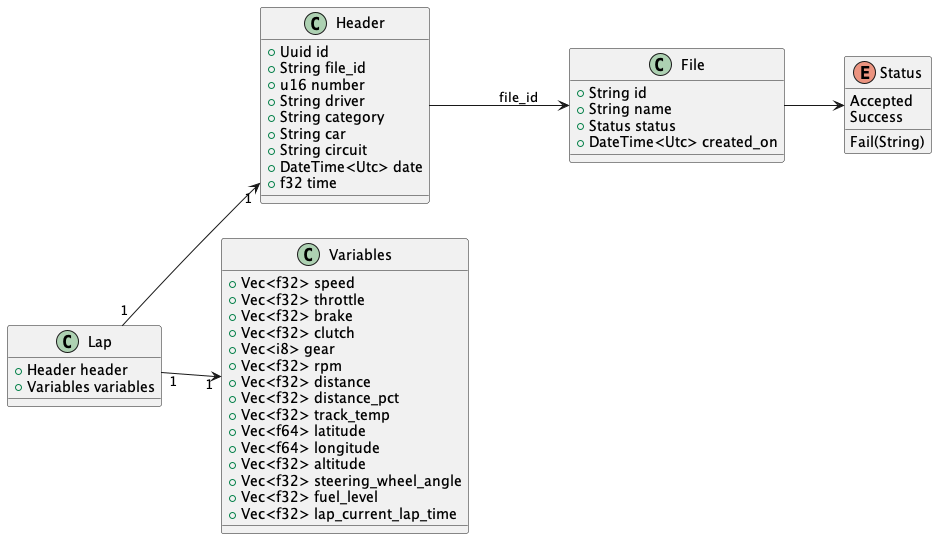
\includegraphics[width=1\linewidth]{./figs/herramientas/desarrollo/modelo_de_datos.png}
	\caption[Modelo de Datos]{Modelo de Datos}
    \label{fig:modelo_de_datos}
\end{figure}

En el diseño del modelo de datos, se tomaron decisiones clave para optimizar la eficiencia y la escalabilidad del sistema. El identificador (id) de cada File se calculó utilizando la función SHA256 sobre los bytes en bruto del fichero, garantizando así unicidad y seguridad. Además, se incluyó un estado (status) en la estructura File, permitiendo gestionar el procesamiento de archivos de manera asíncrona y facilitando la consulta del estado actual de cada archivo.

Se decidió dividir la información de una Lap en dos componentes: cabecera (Header) y datos (Variables). Esta separación permite consultar únicamente las cabeceras sin necesidad de cargar los datos completos, optimizando las consultas y mejorando el rendimiento, dado que los datos son considerablemente más pesados.

La información extraída originalmente del fichero \ac{ibt} almacena los datos en formato de filas, donde cada registro o fila contiene un valor para cada una de las variables medidas, ordenados consecutivamente según las cabeceras. Se implementó un algoritmo (\autoref{alg:from_reader}) para transformar estos datos a un formato columnar, almacenando cada variable en vectores separados. Esto permitió un acceso más eficiente a columnas específicas y optimizó las operaciones de análisis, mejorando el rendimiento del procesamiento de datos.

\IncMargin{1em}
\begin{algorithm}[H]
\SetKwInOut{Input}{Datos}
\SetKwInOut{Output}{Resultado}
\LinesNumbered
\SetAlgoLined

\Input{lector (\texttt{reader}), cabecera (\texttt{header}), filtro (\texttt{filter})}
\Output{Lista de Variables (\texttt{variables})}

\SetKwFunction{FMain}{from\_reader}
\SetKwProg{Fn}{Función}{:}{}

\Fn{\FMain{\texttt{reader}, \texttt{header}, \texttt{filter}}} {
    Leer cabeceras de variables (\texttt{var\_headers}) mediante lector y cabecera\;
    
    Calcular tamaño del bloque de variables (\texttt{var\_block\_size})\;

    \If{filtro está presente (\texttt{filter})} {
        Filtrar cabeceras de variables usando el filtro\;
    }

    \texttt{variables\_result} $\leftarrow$ lista vacía\;

    \ForEach{cabecera de variable en \texttt{var\_headers}} {
        Seleccionar el búfer con el mayor \texttt{tick\_count} de la cabecera\;
        Leer variables mediante lector, cabecera de variable, desplazamiento del búfer y tamaño del bloque de variables\;
        Añadir variable a \texttt{variables\_result}\;
    }

    \Return{Lista de Variables (\texttt{variables\_result})}\;
}
\caption{Conversión de formato \ac{ibt} a formato columnar}\label{alg:from_reader}
\end{algorithm}
\DecMargin{1em}


Las variables relativas al piloto, circuito, fecha y categoría se extrajeron de la información de la sesión utilizando la librería serde\_yaml \cite{serde_yaml}. Se implementaron estructuras de datos que permitían valores nulos, proporcionando flexibilidad para manejar el formato dinámico de almacenamiento del fichero \ac{ibt}. Esta flexibilidad fue crucial para asegurar una correcta interpretación y visualización de los datos extraídos. En el \autoref{alg:ibt_variables2laps} se muestra una parte ilustrativa del algoritmo de extracción.

\IncMargin{1em}
\begin{algorithm}[H]
\SetKwInOut{Input}{Datos}
\SetKwInOut{Output}{Resultado}
\LinesNumbered
\SetAlgoLined

\Input{Identificador de archivo (\texttt{file\_id}), información de la sesión (\texttt{session\_info}), variables extraídas (\texttt{variables})}
\Output{Lista de vueltas (\texttt{laps\_vec})}

\SetKwFunction{FMain}{ibt\_variables2laps}
\SetKwProg{Fn}{Función}{:}{}

\Fn{\FMain{\texttt{file\_id}, \texttt{session\_info}, \texttt{variables}}} {
    Obtener \texttt{driver\_name} de \texttt{session\_info}\;
    
    Obtener \texttt{category} de \texttt{session\_info}\;

    Obtener \texttt{car} de \texttt{session\_info}\;

    Obtener \texttt{circuit} de \texttt{session\_info}\;

    Obtener \texttt{date} de \texttt{session\_info}\;

    Agrupar \texttt{variables} por número de vuelta en \texttt{variables\_by\_lap}\;

    \texttt{laps\_vec} $\leftarrow$ lista vacía\;

    \ForEach{(número\_de\_vuelta, variables) en \texttt{variables\_by\_lap}} {
        Crear nueva vuelta con los parámetros \texttt{file\_id}, \texttt{número\_de\_vuelta}, \texttt{driver\_name}, \texttt{category}, \texttt{car}, \texttt{circuit}, \texttt{date} y \texttt{variables}\;
        Agregar vuelta a \texttt{laps\_vec}\;
    }

    \Return{\texttt{laps\_vec}}\;
}
\caption{Conversión de variables de IBT a vueltas}\label{alg:ibt_variables2laps}
\end{algorithm}
\DecMargin{1em}



\subsection{Validación de datos extraídos en formato tabular}
\begin{table}[H]
\centering
\begin{tabular}{|l|p{10cm}|}
\hline
\multicolumn{2}{|c|}{\textbf{Historia de Usuario 4}} \\ \hline
\textbf{Nombre:} & Validación de datos extraídos en formato tabular \\ \hline
\textbf{Descripción:} & Como cliente del proyecto, quiero visualizar los datos de telemetría extraídos en un formato tabular legible, para facilitar la validación de la información procesada y asegurar su precisión y coherencia. \\ \hline
\textbf{Prioridad:} & P2 \\ \hline
\textbf{Talla:} & S \\ \hline
\textbf{Sprints:} & 9 \\ \hline
\end{tabular}
\caption{Historia de Usuario 4}
\label{tab:us_visualizacion_basica}
\end{table}

Se determinó que, debido a la naturaleza de los datos, el formato \ac{json} es más conveniente que un formato tabular tradicional. Los datos de telemetría contienen múltiples variables con diferentes tipos y tamaños, que se capturan en intervalos muy cortos de tiempo, lo que resulta en un volumen de datos elevado y estructurado de manera compleja. Un formato tabular al uso, como  \ac{csv}, puede resultar en una representación menos clara y más difícil de manejar debido a la extensión horizontal que tendría, al intentar representar cada variable como una columna.

El formato \ac{json}, por otro lado, permite una representación jerárquica y estructurada de los datos, facilitando su organización y lectura. Al utilizar \ac{json}, cada variable de telemetría puede ser representada como una clave con sus valores correspondientes, agrupados de manera que refleje la estructura lógica de los datos. Esto no sólo mejora la legibilidad, sino que también permite una manipulación más eficiente de los datos mediante herramientas y bibliotecas de software comúnmente utilizadas en análisis de datos y desarrollo web.

Para la creación del archivo \ac{json}, se implementó un algoritmo que recorrió la estructura de datos utilizada para almacenar la telemetría extraída. Durante este proceso, los datos fueron escritos directamente en la salida estándar (stdout) en formato \ac{json}, utilizando funciones de serialización disponibles en el lenguaje de programación Rust. Esta metodología garantizó que los datos se capturaran de manera fiel y precisa, permitiendo su validación inmediata. La utilización de stdout para la generación del \ac{json} aseguró que el proceso fuera eficiente y que los datos pudieran ser redirigidos o almacenados según fuera necesario, sin necesidad de almacenamiento intermedio en archivos temporales.

En el \autoref{lst:muestra_datos_extraidos} se muestra un ejemplo del \ac{json} generado, mostrando cómo se estructuraron y visualizaron los datos de telemetría extraídos, asegurando su precisión y coherencia para facilitar su validación.

\newpage

\begin{lstlisting}[label=lst:muestra_datos_extraidos, caption=Muestra \ac{json} de los datos extraídos]
{
  "id": "123e4567-e89b-12d3-a456-426614174000",
  "file_id": 
  "e3b0c44298fc1c149afbf4c8996fb92427ae41e4649b934ca495991b7852b855",
  "number": 1,
  "driver": "John Doe",
  "category": "GT3",
  "car": "Ferrari 488 GT3",
  "circuit": "Monza",
  "date": "2024-06-19T19:15:25.258553Z",
  "time": 85.23,
  "speed": [50.2, 60.4, 70.1],
  "throttle": [0.8, 0.9, 1.0],
  "brake": [0.1, 0.0, 0.2],
  "clutch": [0.0, 0.0, 0.1],
  "gear": [3, 4, 5],
  "rpm": [7000, 7200, 7400],
  "distance": [3000.0, 3100.0, 3200.0],
  "distance_pct": [0.85, 0.88, 0.90],
  "track_temp": [28.0, 28.5, 29.0],
  "latitude": [45.467, 45.468, 45.469],
  "longitude": [9.191, 9.192, 9.193],
  "altitude": [150.0, 155.0, 160.0],
  "steering_wheel_angle": [0.05, 0.04, 0.03],
  "fuel_level": [15.0, 14.5, 14.0],
  "lap_current_lap_time": [85.23, 85.50, 85.75]
}
\end{lstlisting}

\section{Hito 2: Definición de las métricas de comparación \textit{(SO2)}}
El hito implicó un enfoque integral para establecer y comparar el rendimiento entre distintos archivos de telemetría. Inicialmente se identificaron y definieron métricas de rendimiento clave, proporcionando una base sólida para la evaluación. Posteriormente, se desarrollaron algoritmos específicos para calcular y comparar estas métricas, asegurando la precisión y coherencia en el análisis. Finalmente, se implementaron visualizaciones comparativas que permitieron una mejor comprensión y análisis de los datos, facilitando la validación y asegurando la calidad de la información procesada. 

\begin{table}[H]
\centering
\begin{tabular}{|l|c|}
\hline
\textbf{Título} & Definición de las métricas de comparación \\ \hline
\textbf{Código} & \textit{SO2} \\ \hline
\textbf{Historias de Usuario} & 3 \\ \hline
\textbf{Sprints} & 10-19 \\ \hline
\end{tabular}
\caption{Resumen del Hito 2}
\label{tab:resumen_hito_2}
\end{table}

A continuación, se detallan las historias de usuario necesarias para alcanzar el hito de la definición de las métricas de comparación. Estas historias de usuario abarcan la identificación de métricas relevantes, el desarrollo de algoritmos para su cálculo y la implementación de visualizaciones comparativas, garantizando así una evaluación precisa y comprensible del rendimiento.

\subsection{Definir métricas de rendimiento relevantes}
\begin{table}[H]
\centering
\begin{tabular}{|l|p{10cm}|}
\hline
\multicolumn{2}{|c|}{\textbf{Historia de Usuario 5}} \\ \hline
\textbf{Nombre:} & Definir métricas de rendimiento relevantes \\ \hline
\textbf{Descripción:} & Como cliente del proyecto, quiero definir métricas de rendimiento relevantes para comparar diferentes archivos de telemetría, con el fin de evaluar el rendimiento de manera precisa y consistente \\ \hline
\textbf{Prioridad:} & P1 \\ \hline
\textbf{Talla:} & S \\ \hline
\textbf{Sprints:} & 10 \\ \hline
\end{tabular}
\caption{Historia de Usuario 5}
\label{tab:metricas_rendimiento}
\end{table}

En esta historia de usuario se determinó que la métrica adecuada para comparar diferentes vueltas a un circuito sería la diferencia entre las variables de una vuelta de referencia y una vuelta objetivo. La vuelta de referencia, idealmente, corresponde a los tiempos óptimos al recorrer el circuito, mientras que la vuelta objetivo es la que se desea mejorar. Esta métrica es adecuada porque permite evaluar de manera precisa las áreas de mejora, comparando directamente el rendimiento ideal con el actual. Los beneficios incluyen una identificación clara de las diferencias de rendimiento y la focalización en aspectos específicos que necesitan optimización.

Para implementar esta métrica, se tomó como eje de referencia las distancias recorridas en lugar del tiempo. La razón principal es que el tiempo varía entre vueltas, debido a la naturaleza del desempeño del piloto y las condiciones del circuito, mientras que la distancia recorrida es una constante en todas las vueltas. Esto garantiza una comparación justa y precisa entre las vueltas de referencia y las vueltas objetivo.

Dado que la información obtenida de los archivos \ac{ibt} no contiene las distancias estandarizadas, sino que varían dependiendo de la máquina donde se ejecuta, fue necesario realizar un proceso de interpolación. Este proceso involucró calcular todos los puntos de distancia de ambas vueltas y luego interpolar los valores de las variables a estos puntos comunes. Esto permitió una comparación directa y precisa entre los datos de telemetría de las vueltas de referencia y las vueltas objetivo, asegurando que las diferencias en las métricas de rendimiento fueran coherentes y significativas. Este enfoque ha permitido una evaluación detallada y exacta del rendimiento en el simulador de carreras.

\subsection{Desarrollar algoritmos para calcular y comparar métricas}
\begin{table}[H]
\centering
\begin{tabular}{|l|p{10cm}|}
\hline
\multicolumn{2}{|c|}{\textbf{Historia de Usuario 6}} \\ \hline
\textbf{Nombre:} & Desarrollar algoritmos para calcular y comparar métricas \\ \hline
\textbf{Descripción:} & Como cliente del proyecto, quiero que se desarrollen algoritmos que permitan calcular y comparar las métricas de rendimiento entre diferentes archivos de telemetría, con el fin de obtener una evaluación detallada y precisa del rendimiento. \\ \hline
\textbf{Prioridad:} & P1 \\ \hline
\textbf{Talla:} & M \\ \hline
\textbf{Sprints:} & 11-13 \\ \hline
\end{tabular}
\caption{Historia de Usuario 6}
\label{tab:algoritmos_metricas}
\end{table}

Esta historia de usuario se focalizó en implementar algoritmos eficientes que permitieran realizar estas comparaciones de manera efectiva. El primer algoritmo (\autoref{alg:union_distancias}) se centró en la generación de una unión de puntos de distancia entre una vuelta de referencia y una vuelta objetivo. Este algoritmo ordenó y eliminó duplicados de las distancias registradas en ambas vueltas, permitiendo una comparación coherente. Esta unión de puntos es fundamental para normalizar las distancias entre diferentes vueltas, facilitando así una comparación precisa de los datos.

\IncMargin{1em}
\begin{algorithm}[H]
\SetKwInOut{Input}{Datos}
\SetKwInOut{Output}{Resultado}
\LinesNumbered
\SetAlgoLined

\Input{Dos vueltas \texttt{lap1} y \texttt{lap2} con sus distancias correspondientes}
\Output{Un vector de distancias unificadas y ordenadas}

\BlankLine
Inicializar un vector vacío \texttt{distances}\;
\ForEach{distancia en \texttt{lap1.variables.distance}}{
    Añadir la distancia a \texttt{distances}\;
}
\ForEach{distancia en \texttt{lap2.variables.distance}}{
    Añadir la distancia a \texttt{distances}\;
}
Ordenar \texttt{distances} de menor a mayor\;
Eliminar duplicados en \texttt{distances}\;

\BlankLine
\Return \texttt{distances}\;

\caption{Generación de la unión de puntos de distancia entre dos vueltas}
\label{alg:union_distancias}
\end{algorithm}
\DecMargin{1em}

El siguiente paso fue desarrollar un algoritmo (\autoref{alg:interpolacion}) para la interpolación lineal de los valores de las variables en función de las nuevas distancias unificadas. Este algoritmo permitió obtener valores interpolados de las variables tanto para la vuelta de referencia como para la vuelta objetivo, asegurando que los datos se compararan de manera precisa incluso cuando las muestras originales no coincidían en los mismos puntos de distancia.


\IncMargin{1em}
\begin{algorithm}[H]
\SetKwInOut{Input}{Datos}
\SetKwInOut{Output}{Resultado}
\LinesNumbered
\SetAlgoLined

\Input{Valores \texttt{values}, distancias \texttt{distances}, nuevas distancias \texttt{new\_distances}, indicador de discreción \texttt{is\_discrete}}
\Output{Vector de valores interpolados}

Inicializar un vector vacío \texttt{interpolated\_values}\;

\ForEach{\texttt{new\_distance} en \texttt{new\_distances}}{
    Encontrar la posición de \texttt{new\_distance} en \texttt{distances}\;
    \eIf{posición es 0}{
        \texttt{value} = \texttt{values[0]}\;
    }{
        \eIf{posición es igual al tamaño de \texttt{distances}}{
            \texttt{value} = \texttt{values[última posición]}\;
        }{
            \texttt{d0} = \texttt{distances[posición - 1]}\;
            \texttt{d1} = \texttt{distances[posición]}\;
            \texttt{v0} = \texttt{values[posición - 1]}\;
            \texttt{v1} = \texttt{values[posición]}\;

            \texttt{interpolated} = ((\texttt{new\_distance} - \texttt{d0}) / (\texttt{d1} - \texttt{d0})) * (\texttt{v1} - \texttt{v0}) + \texttt{v0}\;

            \eIf{\texttt{is\_discrete}}{
                \texttt{value} = \texttt{round(interpolated)}\;
            }{
                \texttt{value} = \texttt{interpolated}\;
            }
        }
    }
    Añadir \texttt{value} a \texttt{interpolated\_values}\;
}

\BlankLine
\Return \texttt{interpolated\_values}\;

\caption{Interpolación de valores entre la vuelta de referencia y la vuelta objetivo}
\label{alg:interpolacion}
\end{algorithm}
\DecMargin{1em}


Finalmente, se desarrolló un algoritmo para calcular las diferencias entre las variables de la vuelta de referencia y la vuelta objetivo. Este algoritmo comparó las variables interpoladas en cada punto de distancia, proporcionando un conjunto de métricas comparativas. Estas métricas permiten evaluar el rendimiento relativo entre ambas vueltas, identificando las áreas con diferencias significativas.

Todo lo anterior se ha materializado en una estructura de análisis denominada Analysis. Esta estructura encapsula la información y resultados obtenidos durante el proceso de comparación de vueltas.

La estructura Analysis incluye:
\begin{itemize}
    \item \textbf{Header}: Información básica sobre el análisis, como la descripción y metadatos asociados.
    \item \textbf{Reference y Target}: Las vueltas de referencia y objetivo que se están comparando, encapsuladas en la estructura ReferenceLap.
    \item \textbf{Union Distances}: Un vector de distancias comunes interpoladas, utilizado como eje de referencia para comparar las variables de las vueltas.
    \item \textbf{Differences}: Las métricas de diferencias calculadas entre las vueltas de referencia y objetivo, representadas en la estructura Variables.
\end{itemize}


Esta organización ha permitido almacenar y analizar de manera coherente los resultados comparativos, facilitando su interpretación y utilización para mejorar el rendimiento en las estrategias de conducción y configuración del vehículo. En la  \autoref{fig:modelo_de_datos_analisis} se presenta el diagrama de clases que ilustra la estructura y relaciones de la clase Analysis.

\begin{figure}[H]
	\centering
	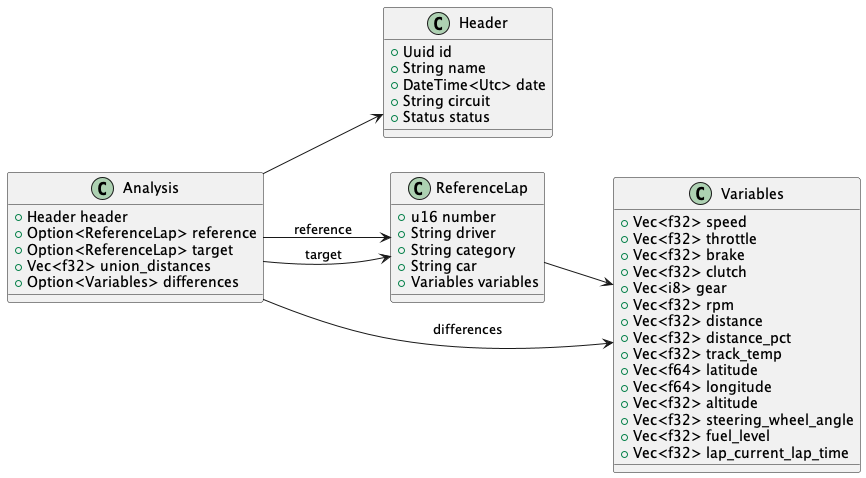
\includegraphics[width=1\linewidth]{./figs/herramientas/desarrollo/modelo_de_datos_analisis.png}
	\caption[Modelo de Datos Datos: Análisis]{Modelo de Datos: Análisis}
    \label{fig:modelo_de_datos_analisis}
\end{figure}

\subsection{Implementar visualizaciones comparativas de métricas}
\begin{table}[H]
\centering
\begin{tabular}{|l|p{10cm}|}
\hline
\multicolumn{2}{|c|}{\textbf{Historia de Usuario 7}} \\ \hline
\textbf{Nombre:} & Implementar visualizaciones comparativas de métricas \\ \hline
\textbf{Descripción:} & Como cliente del proyecto, quiero que se implementen visualizaciones comparativas de las métricas de rendimiento, para facilitar la comprensión y análisis de los datos de telemetría de manera visual y accesible. \\ \hline
\textbf{Prioridad:} & P1 \\ \hline
\textbf{Talla:} & L \\ \hline
\textbf{Sprints:} & 14-19 \\ \hline
\end{tabular}
\caption{Historia de Usuario 7}
\label{tab:metricas_rendimiento}
\end{table}

Para esta historia de usuario, se desarrollaron diversas estrategias para lograr una representación visual accesible y comprensible de los datos de telemetría. Se utilizó plotly.rs \cite{plotly}, una adaptación en Rust de la conocida librería de visualización Plotly en JavaScript \cite{plotly_js}. Inicialmente, se implementaron diagramas de dispersión utilizando la distancia como eje X y las diferentes variables de telemetría en el eje Y. Este enfoque permitió un primer módulo parcialmente funcional y estilizado para visualizar los datos.

Durante la revisión del sprint, el cliente solicitó mejoras significativas: se requería la visualización de las métricas más importantes en gráficos superpuestos, con un indicador sincronizado en todos ellos. Además, se especificó que el zoom debía ser horizontal y sincronizado entre todos los gráficos. Sin embargo, se encontraron varios desafíos técnicos con plotly.rs, ya que no permitía este comportamiento de forma nativa. Se intentó una solución manual, pero plotly.rs sólo permite gestionar eventos mediante \ac{wasm}. Al utilizar \ac{wasm}, se descubrió que los eventos emitidos por plotly no eran reconocidos. Para solucionar este problema, se habría necesitado desarrollar un proyecto completo en \ac{wasm} para gestionar estos eventos.

Para superar estos obstáculos, se decidió implementar la parte de sincronización de zoom e indicadores en JavaScript, estableciendo un enlace con Rust mediante \ac{wasm} para que ambos lenguajes pudieran comunicarse eficientemente. Este enfoque permitió implementar la funcionalidad deseada de manera efectiva.

El \autoref{lst:plotly_js} muestra el código JavaScript que implementa la sincronización del indicador de las gráficas de dispersión de Plotly cuando el puntero del ratón se posiciona sobre ellas.


\begin{lstlisting}[label=lst:plotly_js, caption=Sincronización del indicador cuando el cursor pase por encima]
export function sync_plotly(div_id, sync_div_ids) {
    let dashboardPlot = document.getElementById(div_id);
    let plotsNames = [...Object.keys(dashboardPlot._fullLayout._plots)];
    dashboardPlot.on('plotly_hover', function (event) {
        sync_div_ids.forEach(sync_div_id => {
            let syncPlot = document.getElementById(sync_div_id);
            Plotly.Fx.hover(
                syncPlot,
                { xval: event.xvals[0] },
                plotsNames
            );
            window.wasmBindings.hover_event_from_plotly(
                    event.xvals[0]
                );
        });
    });
}
\end{lstlisting}
\vspace{1em}
El \autoref{lst:wasm_bind} muestra el enlace del código anterior con código Rust mediante \ac{wasm}.

\begin{lstlisting}[language=Rust, label=lst:wasm_bind, caption=Enlace del código JavaScript a Rust mediante \ac{wasm}]
#[wasm_bindgen(module = "/assets/scripts/plotly_interop.js")]
extern "C" {
    #[wasm_bindgen(js_name = "sync_plotly")]
    fn sync_plotly(div_id: JsValue, sync_div_ids: Vec<JsValue>);
}
\end{lstlisting}

Además, se añadió un eje Y adicional a cada diagrama de dispersión para mostrar el vector de diferencias entre ambas vueltas en su escala correspondiente para cada punto de la distancia. En la \autoref{fig:visualizacion} se muestran de forma clara y detallada los puntos con mayor diferencia entre las vueltas.

\begin{figure}[H]
	\centering
	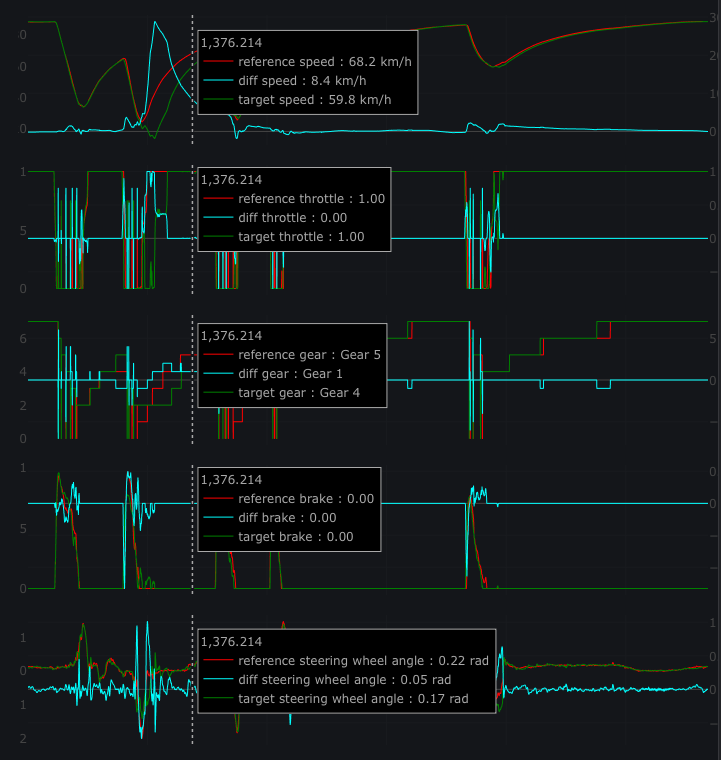
\includegraphics[width=1\linewidth]{./figs/herramientas/desarrollo/visualizacion.png}
	\caption[Visualización de diferencias de variables]{Visualización de diferencias de variables}
    \label{fig:visualizacion}
\end{figure}
\vspace{2em}

\newpage



\section{Hito 3: Aplicación de aprendizaje no supervisado \textit{(SO3)}}

En este hito se implementaron técnicas de aprendizaje no supervisado para clasificar las diferencias de las variables obtenidas de los archivos de telemetría. El objetivo fue identificar patrones y agrupar las diferencias en categorías significativas, permitiendo una evaluación detallada y precisa del rendimiento. Esta clasificación facilitó la interpretación de los datos y mejoró la comprensión de las variaciones en el rendimiento.

\begin{table}[H]
\centering
\begin{tabular}{|l|c|}
\hline
\textbf{Título} & Aplicación de aprendizaje no supervisado \\ \hline
\textbf{Código} & \textit{SO3} \\ \hline
\textbf{Historias de Usuario} & 3 \\ \hline
\textbf{Sprints} & 20-26 \\ \hline
\end{tabular}
\caption{Resumen de la sección: Aplicación de aprendizaje no supervisado}
\label{tab
}
\end{table}

A lo largo de este hito, se identificaron y evaluaron varios algoritmos de agrupamiento para seleccionar el más adecuado para clasificar las diferencias de variables. Se desarrollaron e implementaron algoritmos específicos para agrupar estas diferencias en categorías ordenadas y se abordaron problemas inherentes a los métodos seleccionados. Finalmente, se aplicaron técnicas avanzadas para mejorar la precisión y utilidad de las categorías generadas, asegurando una clasificación más precisa y adaptable de los datos de telemetría. A continuación, se detallan las historias de usuario que conformaron el hito.

\subsection{Identificación de algoritmos de agrupamiento apropiados}
\begin{table}[H]
\centering
\begin{tabular}{|l|p{10cm}|}
\hline
\multicolumn{2}{|c|}{\textbf{Historia de Usuario 8}} \\ \hline
\textbf{Nombre:} & Identificación de algoritmos de agrupamiento apropiados \\ \hline
\textbf{Descripción:} & Como cliente del proyecto, quiero identificar los algoritmos de agrupamiento más adecuados para clasificar las métricas de diferencias de las variables de telemetría, con el fin de obtener agrupamientos precisos y útiles para el análisis de rendimiento. \\ \hline
\textbf{Prioridad:} & P1 \\ \hline
\textbf{Talla:} & M \\ \hline
\textbf{Sprints:} & 20-21 \\ \hline
\end{tabular}
\caption{Historia de Usuario 8}
\label{tab:identificar_algoritmos_agrupamiento}
\end{table}

Para clasificar los vectores de diferencias en las variables de telemetría, se evaluó inicialmente el uso del algoritmo K-means debido a su simplicidad, eficiencia y capacidad para crear categorías ordenadas. K-means agrupa datos en un número predefinido de agrupaciones, donde cada punto de datos pertenece al grupo cuyo centroide es el más cercano. Este algoritmo minimiza la variabilidad dentro de cada agrupación, asegurando que los puntos de datos dentro de un grupo sean lo más similares posible. El \autoref{alg:k-means} muestra el algoritmo K-means.

\IncMargin{1em}
\begin{algorithm}[H]
\SetKwInOut{Input}{Datos}\SetKwInOut{Output}{Resultado}
\LinesNumbered
\SetAlgoLined

\Input{Conjunto de datos $\mathbf{X}$, número de clusters $k$}
\Output{Conjunto de centroides $\mathbf{C}$, asignaciones de clusters $\mathbf{A}$}

Inicializar aleatoriamente los centroides $\mathbf{C}$;
\Repeat{convergencia}{
\ForEach{punto de datos $\mathbf{x}_i$}{
Asignar el punto de datos al cluster más cercano $a_i = \arg\min_j |\mathbf{x}_i - \mathbf{c}_j|$;
}
\ForEach{cluster $j$}{
Actualizar el centroide $\mathbf{c}j = \frac{1}{|C_j|} \sum{\mathbf{x}_i \in C_j} \mathbf{x}_i$;
}
}
\caption{Algoritmo K-means}\label{alg
}
\label{alg:k-means}
\end{algorithm}
\DecMargin{1em}

La característica de K-means de ordenar las categorías es especialmente útil para clasificar diferencias en las variables de telemetría. Por ejemplo, si se determina que el número óptimo de clusters es cinco (k=5), las categorías podrían ser: ``Mucha Diferencia Negativa'', ``Diferencia Negativa'', '``No diferencia'', ``Diferencia Positiva'' y ``Mucha Diferencia Positiva''. En este caso, el primer grupo tendría centroides más cercanos a las diferencias negativas con menor valor, y así sucesivamente, asegurando que las categorías estén ordenadas de manera coherente.

\subsubsection*{Problemas identificados con K-means}
Sin embargo, K-means presenta ciertas limitaciones al crear clases cerradas. En particular, cuando los puntos de datos están cerca de los límites de dos clases, el algoritmo fuerza a que pertenezcan exclusivamente a una de ellas. Por ejemplo, si consideramos la variable velocidad y un punto de la diferencia de velocidad que está casi equidistante a los centroides de las clases ``No Diferencia'' y ``Diferencia Negativa", K-means asignaría el punto a una de las dos clases, perdiendo la información sobre su cercanía a ambas. La \autoref{fig:problemas_kmeans} refleja este problema.

\begin{figure}[H]
\centering
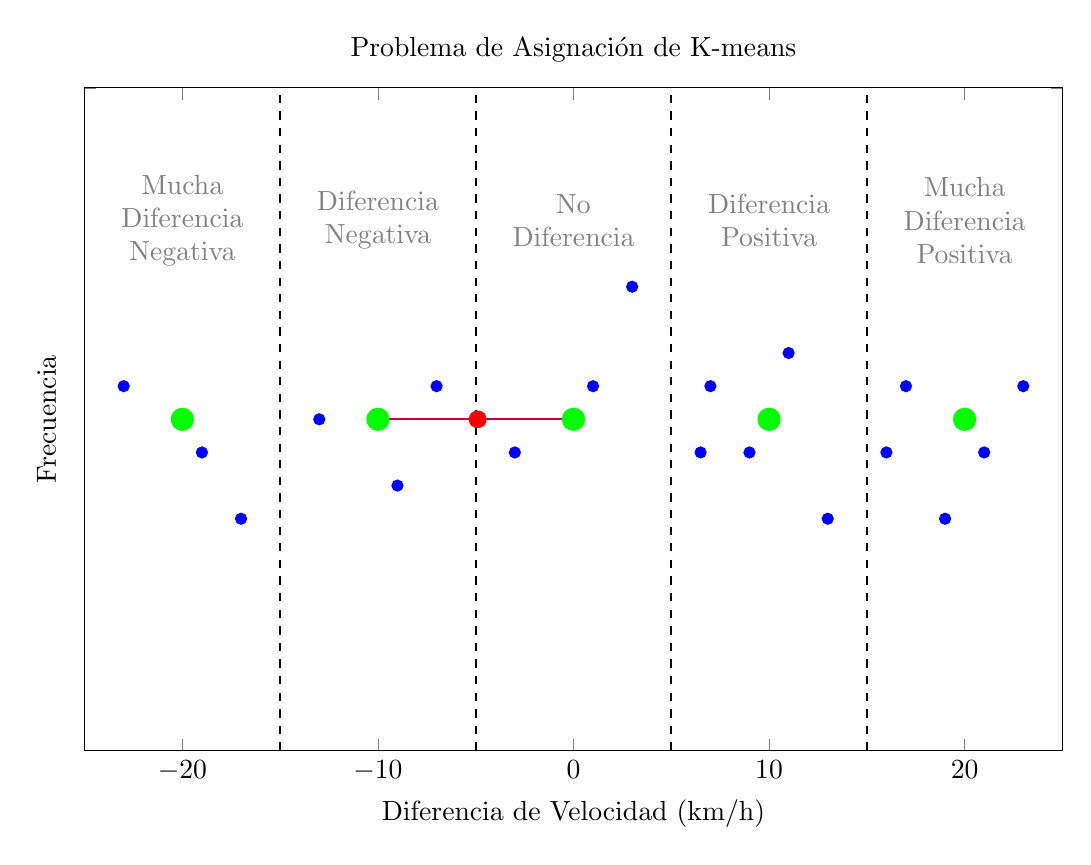
\begin{tikzpicture}
\begin{axis}[
    title={Problema de Asignación de K-means},
    xlabel={Diferencia de Velocidad (km/h)},
    ylabel={Frecuencia},
    ytick={\empty},
    xtick={-20, -10, 0, 10, 20},
    ymajorgrids=true,
    grid style=dashed,
    xmin=-25, xmax=25,
    ymin=0, ymax=1,
    enlargelimits=false,
    clip=false,
    width=14cm,
    height=10cm,
    extra y ticks={1},
    extra y tick labels={},
    extra y tick style={grid=none}
]

% Dibujar puntos de clusters
\addplot[
    only marks,
    mark=*,
    color=blue
    ]
    coordinates {
    (-23, 0.55)
    (-19, 0.45)
    (-17, 0.35)
    (-13, 0.5)
    (-9, 0.4)
    (-7, 0.55)
    (-3, 0.45)
    (1, 0.55)
    (3, 0.7)
    (6.5, 0.45)
    (7, 0.55)
    (9, 0.45)
    (11, 0.6)
    (13, 0.35)
    (16, 0.45)
    (17, 0.55)
    (19, 0.35)
    (21, 0.45)
    (23, 0.55)
    };

% Añadir el punto en cuestión
\addplot[
    only marks,
    mark=*,
    mark options={scale=1.5, fill=red},
    color=red
    ]
    coordinates {
    (-4.9, 0.5)
    };

% Añadir centroides
\addplot[
    only marks,
    mark=*,
    mark options={scale=2, fill=green},
    color=green
    ]
    coordinates {
    (-20, 0.5)
    (-10, 0.5)
    (0, 0.5)
    (10, 0.5)
    (20, 0.5)
    };

% Líneas de delimitación de clusters
\draw[dashed, thick] (axis cs:-15,0) -- (axis cs:-15,1);
\draw[dashed, thick] (axis cs:-5,0) -- (axis cs:-5,1);
\draw[dashed, thick] (axis cs:5,0) -- (axis cs:5,1);
\draw[dashed, thick] (axis cs:15,0) -- (axis cs:15,1);

% Flechas de doble punta
\draw[<->, thick, color=purple] (axis cs:-4.9,0.5) -- (axis cs:-10,0.5);
\draw[<->, thick, color=purple] (axis cs:-4.9,0.5) -- (axis cs:0,0.5);

% Etiquetas de las categorías dentro de la gráfica
\node[align=center, text=gray] at (axis cs:-20,0.8) {Mucha\\Diferencia\\Negativa};
\node[align=center, text=gray] at (axis cs:-10,0.8) {Diferencia\\Negativa};
\node[align=center, text=gray] at (axis cs:0,0.8) {No\\Diferencia};
\node[align=center, text=gray] at (axis cs:10,0.8) {Diferencia\\Positiva};
\node[align=center, text=gray] at (axis cs:20,0.8) {Mucha\\Diferencia\\Positiva};

\end{axis}
\end{tikzpicture}
\caption{Ejemplo de un punto cercano al límite entre las categorías de K-means}
\label{fig:problemas_kmeans}
\end{figure}

\subsubsection*{Resolviendo el problema mediante conjuntos difusos}
Para resolver este problema, se planteó el uso de conjuntos difusos, donde cada punto de datos puede pertenecer a múltiples clases con diferentes niveles de pertenencia. Esto permite una representación más precisa de los puntos que están en los límites de las clases. En la \autoref{fig:conjuntos_difusos} se puede ver como utilizando conjuntos difusos se captura la pertenencia a dos conjuntos, evitando la polarización de K-means.

\begin{figure}[H]
    \centering
    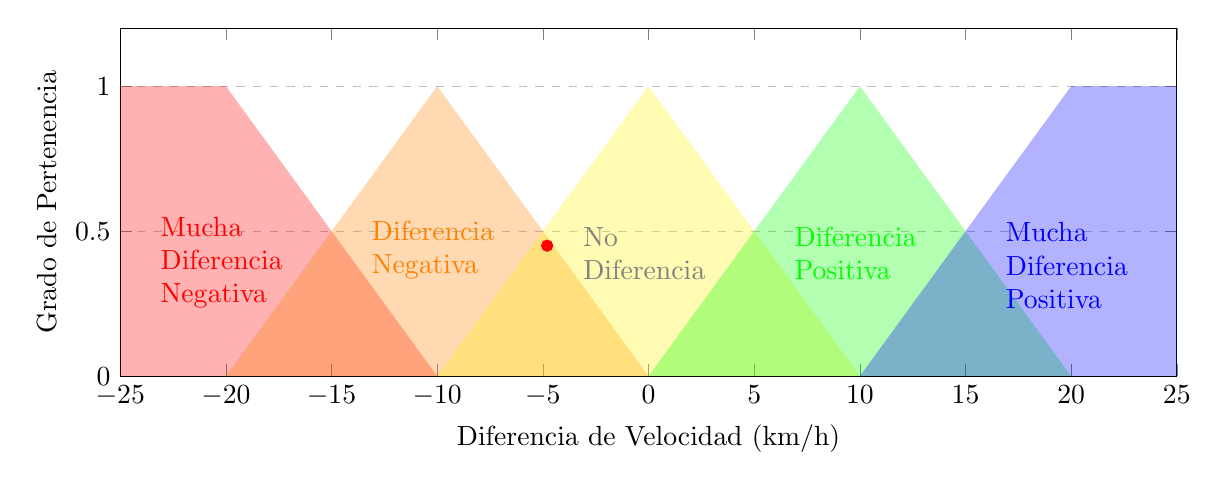
\begin{tikzpicture}
        \begin{axis}[
            width=15cm,
            height=6cm,
            xlabel={Diferencia de Velocidad (km/h)},
            ylabel={Grado de Pertenencia},
            xmin=-25, xmax=25,
            ymin=0, ymax=1.2,
            xtick={-25,-20,-15,-10,-5,0,5,10,15,20,25},
            ytick={0,0.5,1},
            ymajorgrids=true,
            grid style=dashed,
            no markers,
        ]

        % Conjuntos difusos con colores y opacidad
        \addplot[fill=red, fill opacity=0.3, draw=none] coordinates {(-25,1) (-20,1) (-10,0)} \closedcycle;
        \addplot[fill=orange, fill opacity=0.3, draw=none] coordinates {(-20,0) (-10,1) (0,0)} \closedcycle;
        \addplot[fill=yellow, fill opacity=0.3, draw=none] coordinates {(-10,0) (0,1) (10,0)} \closedcycle;
        \addplot[fill=green, fill opacity=0.3, draw=none] coordinates {(0,0) (10,1) (20,0)} \closedcycle;
        \addplot[fill=blue, fill opacity=0.3, draw=none] coordinates {(10,0) (20,1) (25,1)} \closedcycle;

        % Punto de pertenencia difusa
        \addplot[only marks, mark=*, red] coordinates {(-4.8,0.45)};

        % Etiquetas de las categorías
        \node[anchor=south, align=center] at (axis cs:-17.5,0.2) {\textcolor{red}{\parbox{3cm}{Mucha \\ Diferencia \\ Negativa}}};
        \node[anchor=south, align=center] at (axis cs:-7.5,0.3) {\textcolor{orange}{\parbox{3cm}{Diferencia \\ Negativa}}};
        \node[anchor=south, align=center] at (axis cs:2.5,0.3) {\textcolor{gray}{\parbox{3cm}{No \\ Diferencia}}}; % Etiqueta en tono más oscuro
        \node[anchor=south, align=center] at (axis cs:12.5,0.3) {\textcolor{green}{\parbox{3cm}{Diferencia \\ Positiva}}};
        \node[anchor=south, align=center] at (axis cs:22.5,0.2) {\textcolor{blue}{\parbox{3cm}{Mucha \\ Diferencia \\ Positiva}}};
        
        \end{axis}
    \end{tikzpicture}
    \caption{Conjuntos difusos aplicados a la diferencia de velocidad, con un punto ilustrativo.}
    \label{fig:conjuntos_difusos}
\end{figure}

Se consideró la posibilidad de realizar una clasificación difusa a partir de las agrupaciones generadas por K-means, lo que implicaba calcular el grado de pertenencia de cada punto a múltiples categorías. Este enfoque requería un procesamiento adicional para calcular las pertenencias difusas después de la clasificación inicial, lo que incrementaba significativamente el coste computacional y la complejidad de implementación.

En lugar de ello, se optó por utilizar directamente el algoritmo \ac{fcm}, que integra la clasificación difusa desde el principio. \ac{fcm} asigna a cada punto un grado de pertenencia a todas las categorías, reflejando de manera más precisa la incertidumbre inherente en los datos cercanos a los límites de las categorías. Esto no sólo redujo el coste computacional al eliminar la necesidad de un post-procesamiento adicional, sino que también simplificó la implementación y mejoró el rendimiento general del sistema al evitar duplicidades en el cálculo de pertenencias difusas. El \autoref{alg:fcm} muestra el funcionamiento de \ac{fcm}.

\IncMargin{1em}
\begin{algorithm}
\SetKwInOut{Input}{Datos}\SetKwInOut{Output}{Resultado}
\LinesNumbered
\SetAlgoLined

\Input{Conjunto de datos $\mathbf{X}$, número de clusters $C$, parámetro de difusidad $m$}
\Output{Matriz de pertenencia $\mathbf{U}$, centroides $\mathbf{V}$}

Inicializar aleatoriamente la matriz de pertenencia $\mathbf{U}$;
\Repeat{convergencia}{
Calcular los centroides $\mathbf{V}j = \frac{\sum{i=1}^{n} u_{ij}^m \mathbf{x}_i}{\sum{i=1}^{n} u_{ij}^m}$;\\
\ForEach{punto de datos $\mathbf{x}_i$}{
\ForEach{cluster $j$}{
Actualizar la pertenencia $u_{ij} = \frac{1}{\sum_{k=1}^{C} \left( \frac{||\mathbf{x}_i - \mathbf{v}_j||}{||\mathbf{x}_i - \mathbf{v}_k||} \right)^{\frac{2}{m-1}}}$;
}
}
}
\caption{Algoritmo Fuzzy C-means}\label{alg
}
\label{alg:fcm}
\end{algorithm}
\DecMargin{1em}

Por ejemplo, considerando nuevamente la variable velocidad, si un punto de diferencia de velocidad pertenece parcialmente a las clases ``No Diferencia'' y ``Diferencia Negativa'', \ac{fcm} asignaría niveles de pertenencia como 0.45 y 0.55 respectivamente. Esto refleja más adecuadamente la realidad del punto de datos y permite un análisis más detallado y preciso. La \autoref{fig:soluciones_fcm} muestra gráficamente la solución al problema planteado en la \autoref{fig:problemas_kmeans}. 

\begin{figure}[H]
\centering
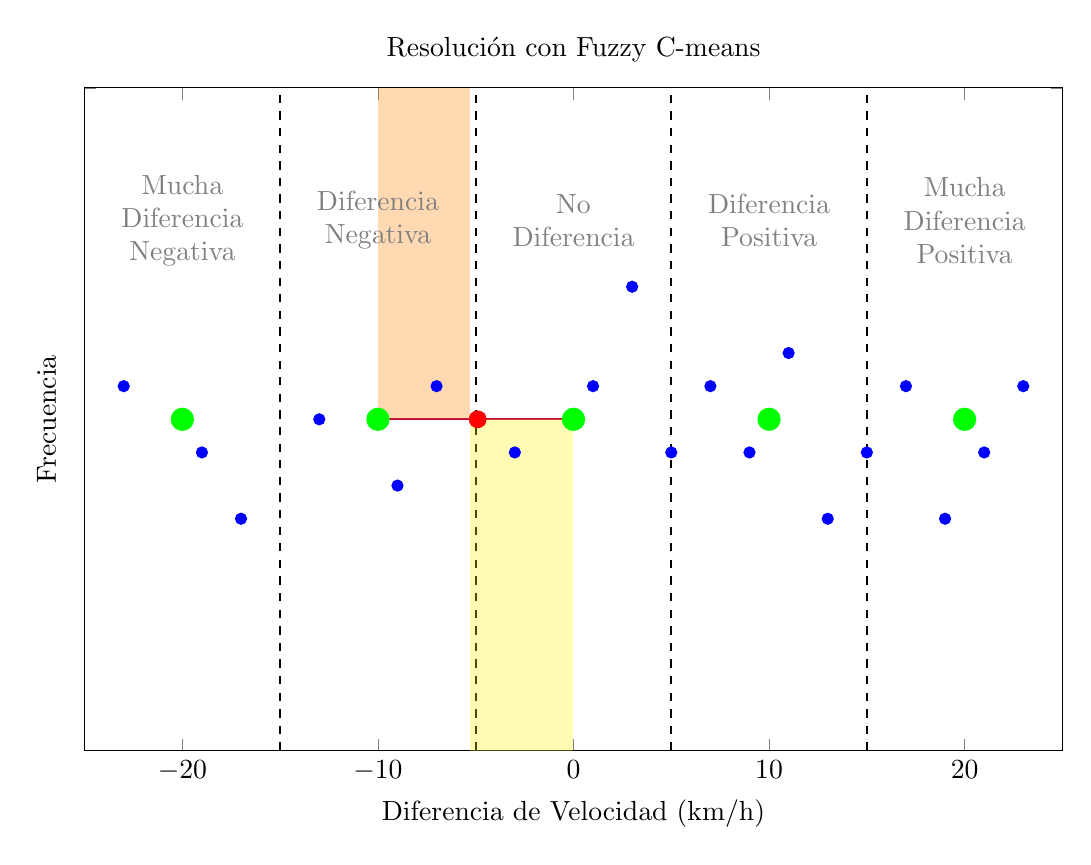
\begin{tikzpicture}
\begin{axis}[
    title={Resolución con Fuzzy C-means},
    xlabel={Diferencia de Velocidad (km/h)},
    ylabel={Frecuencia},
    ytick={\empty},
    xtick={-20, -10, 0, 10, 20},
    ymajorgrids=true,
    grid style=dashed,
    xmin=-25, xmax=25,
    ymin=0, ymax=1,
    enlargelimits=false,
    clip=false,
    width=14cm,
    height=10cm,
    extra y ticks={1},
    extra y tick labels={},
    extra y tick style={grid=none}
]

% Dibujar puntos de clusters
\addplot[
    only marks,
    mark=*,
    color=blue
    ]
    coordinates {
    (-23, 0.55)
    (-19, 0.45)
    (-17, 0.35)
    (-13, 0.5)
    (-9, 0.4)
    (-7, 0.55)
    (-3, 0.45)
    (1, 0.55)
    (3, 0.7)
    (5, 0.45)
    (7, 0.55)
    (9, 0.45)
    (11, 0.6)
    (13, 0.35)
    (15, 0.45)
    (17, 0.55)
    (19, 0.35)
    (21, 0.45)
    (23, 0.55)
    };

% Añadir el punto en cuestión
\addplot[
    only marks,
    mark=*,
    mark options={scale=1.5, fill=red},
    color=red
    ]
    coordinates {
    (-4.9, 0.5)
    };

% Añadir centroides
\addplot[
    only marks,
    mark=*,
    mark options={scale=2, fill=green},
    color=green
    ]
    coordinates {
    (-20, 0.5)
    (-10, 0.5)
    (0, 0.5)
    (10, 0.5)
    (20, 0.5)
    };

% Líneas de delimitación de clusters
\draw[dashed, thick] (axis cs:-15,0) -- (axis cs:-15,1);
\draw[dashed, thick] (axis cs:-5,0) -- (axis cs:-5,1);
\draw[dashed, thick] (axis cs:5,0) -- (axis cs:5,1);
\draw[dashed, thick] (axis cs:15,0) -- (axis cs:15,1);

% Flechas de doble punta
\draw[<->, thick, color=purple] (axis cs:-4.9,0.5) -- (axis cs:-10,0.5);
\draw[<->, thick, color=purple] (axis cs:-4.9,0.5) -- (axis cs:0,0.5);

% Representación de pertenencia difusa
\fill[opacity=0.3, color=yellow] (axis cs:-5.3, 0) rectangle (axis cs:0, 0.5);
\fill[opacity=0.3, color=orange] (axis cs:-5.3, 0.5) rectangle (axis cs:-10, 1);

% Etiquetas de las categorías dentro de la gráfica
\node[align=center, text=gray] at (axis cs:-20,0.8) {Mucha\\Diferencia\\Negativa};
\node[align=center, text=gray] at (axis cs:-10,0.8) {Diferencia\\Negativa};
\node[align=center, text=gray] at (axis cs:0,0.8) {No\\Diferencia};
\node[align=center, text=gray] at (axis cs:10,0.8) {Diferencia\\Positiva};
\node[align=center, text=gray] at (axis cs:20,0.8) {Mucha\\Diferencia\\Positiva};

\end{axis}
\end{tikzpicture}
\caption{Resolución de la asignación con conjuntos difusos usando Fuzzy C-means}
\label{fig:soluciones_fcm}
\end{figure}

\subsection{Configuración de parámetros del algoritmo de agrupamiento}
\begin{table}[H]
\centering
\begin{tabular}{|l|p{10cm}|}
\hline
\multicolumn{2}{|c|}{\textbf{Historia de Usuario 9}} \\ \hline
\textbf{Nombre:} & Configuración de parámetros del algoritmo de agrupamiento \\ \hline
\textbf{Descripción:} & Como cliente del proyecto, quiero configurar los parámetros del algoritmo de agrupamiento seleccionado para optimizar la clasificación de las diferencias en las métricas de telemetría, con el fin de obtener resultados precisos y útiles para el análisis de rendimiento. \\ \hline
\textbf{Prioridad:} & P2 \\ \hline
\textbf{Talla:} & M \\ \hline
\textbf{Sprints:} & 22-23 \\ \hline
\end{tabular}
\caption{Historia de Usuario 9}
\label{tab:configurar_algoritmos_agrupamiento}
\end{table}


En esta historia de usuario se abordó la optimización de los parámetros del algoritmo \ac{fcm} para clasificar eficazmente las diferencias en las métricas de telemetría. El objetivo fue obtener una clasificación precisa y útil para el análisis de rendimiento.

Inicialmente, el cliente propuso permitir que los usuarios configuraran los parámetros del algoritmo de agrupamiento. Sin embargo, se determinó que esta opción requería un control exhaustivo de las entradas del usuario para evitar configuraciones inadecuadas que podrían comprometer la precisión del análisis. Por esta razón, se decidió postergar esta funcionalidad para futuras implementaciones.

En su lugar, se optó por automatizar la configuración de los parámetros utilizando el \ac{fpc} como criterio de optimización. El \ac{fpc} es una medida utilizada en el análisis de conglomerados difusos para evaluar la calidad de las particiones generadas por el algoritmo \ac{fcm}. Este coeficiente varía entre 0 y 1, donde valores más altos indican una mejor definición de los conglomerados, es decir, una menor superposición entre ellos. Un \ac{fpc} cercano a 1 sería ideal, indicando particiones de alta calidad con mínima superposición entre los grupos. La \autoref{fig:fpc} muestra un ejemplo de distintos valores de \ac{fpc} en función de sus parámetros.

\begin{figure}[H]
    \centering
    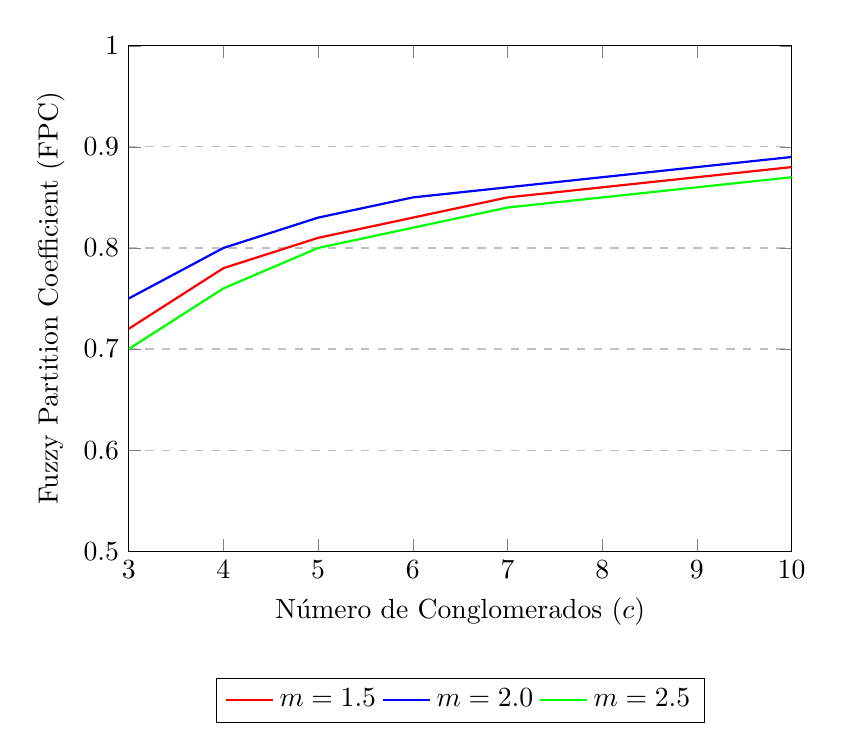
\begin{tikzpicture}
        \begin{axis}[
            width=10cm,
            height=8cm,
            xlabel={Número de Conglomerados ($c$)},
            ylabel={Fuzzy Partition Coefficient (FPC)},
            xmin=3, xmax=10,
            ymin=0.5, ymax=1,
            xtick={3,4,5,6,7,8,9,10},
            ytick={0.5,0.6,0.7,0.8,0.9,1},
            ymajorgrids=true,
            grid style=dashed,
            legend style={at={(0.5,-0.25)}, anchor=north, legend columns=-1},
            no markers,
        ]
        % FPC para m = 1.5
        \addplot[
            color=red,
            thick,
        ] coordinates {
            (3,0.72) (4,0.78) (5,0.81) (6,0.83) (7,0.85) (8,0.86) (9,0.87) (10,0.88)
        };
        % FPC para m = 2.0
        \addplot[
            color=blue,
            thick,
        ] coordinates {
            (3,0.75) (4,0.80) (5,0.83) (6,0.85) (7,0.86) (8,0.87) (9,0.88) (10,0.89)
        };
        % FPC para m = 2.5
        \addplot[
            color=green,
            thick,
        ] coordinates {
            (3,0.70) (4,0.76) (5,0.80) (6,0.82) (7,0.84) (8,0.85) (9,0.86) (10,0.87)
        };
        
        \legend{$m=1.5$,$m=2.0$,$m=2.5$}
        \end{axis}
    \end{tikzpicture}
    \caption{Fuzzy Partition Coefficient (FPC) en función del número de conglomerados ($c$) para diferentes valores de $m$.}
    \label{fig:fpc}
\end{figure}

El algoritmo \ac{fcm} tiene varios parámetros que influyen en su desempeño:

\begin{itemize}
    \item \textbf{Número de conglomerados ($c$)}: Este parámetro determina el número de categorías que se utilizarán para clasificar los datos. Es crucial seleccionar un número apropiado de conglomerados para capturar adecuadamente la estructura subyacente de los datos. En esta implementación, se evaluó típicamente entre 3 y 10, ya que tener sólo dos conglomerados no suele ser conveniente. Con solo dos conglomerados, la capacidad del algoritmo para capturar la diversidad y las variaciones en los datos es limitada, lo que puede llevar a una interpretación demasiado simplificada y posiblemente incorrecta de los datos.
    \item \textbf{Exponente de difusividad ($m$)}: Este parámetro controla el grado de difusividad de la pertenencia de los puntos a los conglomerados. Valores más altos de $m$ resultan en conglomerados más difusos. El valor de $m$ se evaluó en un rango de 1.3 a 2.5. Este rango se seleccionó por las siguientes razones:
    \begin{itemize}
        \item \textit{Claridad en la difusividad}: Valores de $m$ mayores a 2.5 tienden a producir conglomerados excesivamente difusos, disminuyendo la capacidad del algoritmo para identificar claramente las diferencias entre los grupos.
        \item \textit{Estabilidad de la clasificación}: Valores más altos pueden hacer que la clasificación sea más sensible a pequeñas variaciones en los datos, resultando en una menor estabilidad en la asignación de pertenencias.
        \item \textit{Rendimiento computacional}: Valores de $m$ más altos incrementan la complejidad computacional del algoritmo FCM. Al limitar el rango de 1,3 a 2.5, se logra un mejor rendimiento computacional sin sacrificar la calidad de los resultados.
    \end{itemize}
    \item \textbf{Criterio de convergencia}: Este parámetro, también conocido como parámetro de error, define cuándo debe detenerse el algoritmo. Normalmente, se utiliza un umbral pequeño ($\epsilon$), y el algoritmo se detiene cuando la mejora en la función objetivo entre iteraciones sucesivas es menor que este umbral. En esta implementación, se utilizó un rango de valores para $\epsilon$ entre $10^{-4}$ y $10^{-6}$ para asegurar una convergencia precisa.
    \item \textbf{Número máximo de iteraciones}: Este parámetro limita el número de iteraciones del algoritmo para prevenir ciclos infinitos. Se seleccionó un rango de valores entre 500 y 1000 iteraciones, asegurando suficiente tiempo para la convergencia sin extender innecesariamente el tiempo de cálculo.
\end{itemize}

El coeficiente de partición difusa (\ac{fpc}) se calcula utilizando la siguiente fórmula:
\[
\text{FPC} = \frac{1}{n} \sum_{i=1}^{n} \sum_{j=1}^{c} u_{ij}^2
\]
donde:
\begin{itemize}
    \item \( n \) es el número de puntos de datos,
    \item \( c \) es el número de clusters,
    \item \( u_{ij} \) es el grado de pertenencia del punto de datos \( i \) al cluster \( j \).
\end{itemize}


Para seleccionar automáticamente los valores óptimos de estos parámetros, se realizó una búsqueda en un rango apropiado. El valor óptimo de $c$ y $m$ fue el que maximizó el FPC, asegurando así la mejor calidad de las particiones difusas generadas por el algoritmo.

Mediante esta configuración automática, se garantizó que los parámetros del algoritmo FCM estuvieran optimizados para producir clasificaciones precisas y útiles, sin necesidad de intervención manual por parte del usuario. Este enfoque no sólo mejoró la precisión del análisis de telemetría, sino que también simplificó el proceso para los usuarios, asegurando resultados consistentes y de alta calidad.

\subsection{Implementación del algoritmo de Agrupamiento}
\begin{table}[H]
\centering
\begin{tabular}{|l|p{10cm}|}
\hline
\multicolumn{2}{|c|}{\textbf{Historia de Usuario 10}} \\ \hline
\textbf{Nombre:} &  Implementación del algoritmo de Agrupamiento \\ \hline
\textbf{Descripción:} & Como cliente del proyecto, quiero implementar el algoritmo de agrupamiento seleccionado para clasificar las diferencias en las métricas de telemetría, con el fin de obtener una representación precisa de los patrones de rendimiento.  \\ \hline
\textbf{Prioridad:} & P1 \\ \hline
\textbf{Talla:} & L \\ \hline
\textbf{Sprints:} & 24-26 \\ \hline
\end{tabular}
\caption{Historia de Usuario 10}
\label{tab:implementar_algoritmos_agrupamiento}
\end{table}

En esta historia de usuario, se llevó a cabo la implementación del algoritmo de agrupamiento \ac{fcm} en Rust. Dado que no existía una implementación disponible en crates.io \cite{cratesio}, se decidió desarrollar una propia. Este algoritmo es fundamental para clasificar las diferencias en las métricas de telemetría, proporcionando una representación precisa de los patrones de rendimiento.
\newpage
Para implementar el algoritmo, se diseñó una estructura que permitiera inicializar los centroides y calcular los valores de pertenencia de cada punto de datos. Los centroides se inicializaron aleatoriamente a partir de los datos disponibles, logrando una distribución inicial diversificada. Luego, se actualizaban iterativamente los valores de pertenencia y los centroides. Dichos valoes de pertenencia se calculaban basándose en la distancia de cada punto a los centroides, ponderada por el parámetro de fuzziness \( m \). Los centroides se actualizaban calculando el promedio ponderado de los puntos, con los valores de pertenencia elevadas al parámetro \( m \). Este proceso se repetía hasta que la variación máxima en la posición de los centroides fuera menor que un umbral de tolerancia predefinido o hasta alcanzar un número máximo de iteraciones.


Para garantizar una configuración óptima de los parámetros del algoritmo, se empleó una búsqueda exhaustiva de combinaciones de parámetros. Este enfoque permitió explorar sistemáticamente diferentes combinaciones de parámetros, como el número de clusters \( c \) y el parámetro de fuzziness \( m \). El objetivo era maximizar el coeficiente de partición difusa (FPC), el cual mide la calidad de la partición obtenida. Los valores de \( c \) se evaluaron en un rango adecuado para reflejar la variabilidad en las diferencias de las métricas, mientras que los valores de \( m \) se probaron en un rango de 1,5 a 2,5, ya que se consideró que fuera de este rango los resultados eran menos fiables.

\begin{algorithm}[H]
    \SetKwInOut{Input}{Entrada}
    \SetKwInOut{Output}{Salida}
    \SetAlgoLined
    \Input{Datos de telemetría, rangos de parámetros \( c \), \( m \), iteraciones, tolerancia}
    \Output{Parámetros óptimos \( c \), \( m \), iteraciones, tolerancia, máxima FPC}
    \BlankLine
    \For{cada valor de \( c \) en el rango}{
        \For{cada valor de \( m \) en el rango}{
            \For{cada valor de iteraciones en el rango}{
                \For{cada valor de tolerancia en el rango}{
                    Inicializar los centroides aleatoriamente\;
                    \Repeat{criterio de convergencia o máximo de iteraciones}{
                        Actualizar los valores de pertenencia\;
                        Actualizar los centroides\;
                    }
                    Calcular la FPC para esta combinación de \( c \), \( m \), iteraciones y tolerancia\;
                    \If{FPC actual > máxima FPC}{
                        Guardar esta combinación como la mejor encontrada\;
                    }
                }
            }
        }
    }
    \caption{Optimización de parámetros para \ac{fcm}}
    \label{alg:fcm_params}
\end{algorithm}

La implementación también consideró criterios de convergencia estrictos para garantizar resultados precisos. Se estableció un número máximo de iteraciones entre 500 y 1000, y se utilizó un valor de tolerancia en el criterio de convergencia que equilibraba la precisión y la eficiencia computacional. La \autoref{fig:grid_search} muestra algunos ejemplos de los parámetros probados.

\begin{figure}[H]
	\centering
	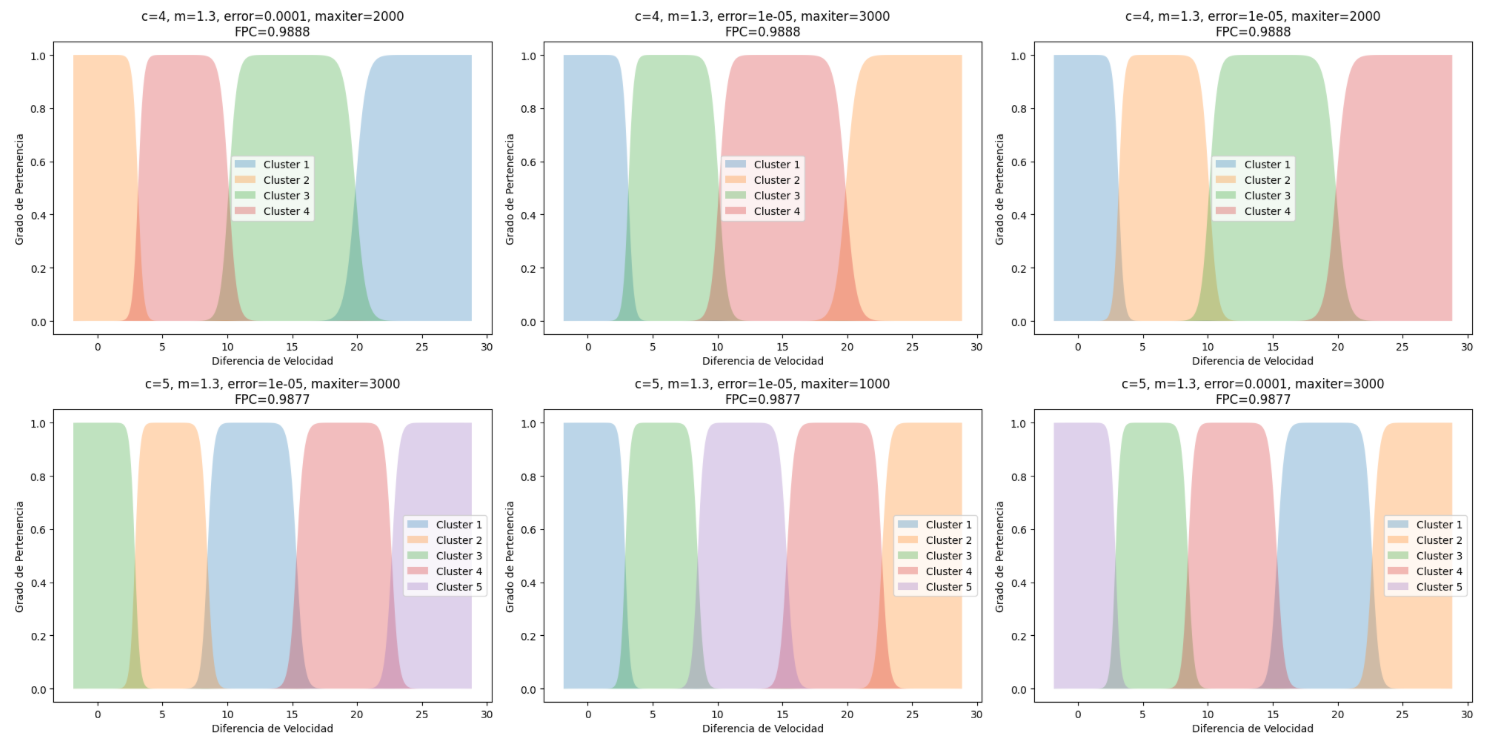
\includegraphics[width=1\linewidth]{./figs/herramientas/desarrollo/grid_search.png}
	\caption[Ejemplo de parámetros de \ac{fcm} probados]{Ejemplo de parámetros de \ac{fcm} probados}
    \label{fig:grid_search}
\end{figure}
\vspace{2em}

Una vez implementado y aplicado el algoritmo de \ac{fcm} a las diferentes métricas de telemetría, se añadió la información del agrupamiento resultante a la estructura de datos en Rust denominada 'Analysis'. Este nuevo añadido permitió almacenar para cada punto de las distancias comunes cuales son los distintos valores de pertenencia a cada una de las agrupaciones. En la \autoref{fig:modelo_de_datos_clustering} se muestra un diagrama de esta estructura, ilustrando cómo se integra la información del agrupamiento con la estructura de datos ya existente.

\begin{figure}[H]
	\centering
	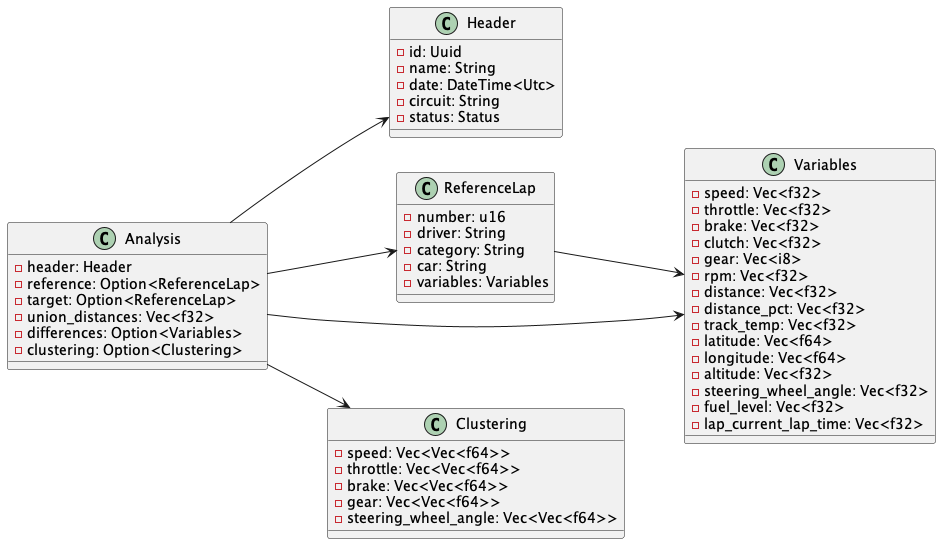
\includegraphics[width=1\linewidth]{./figs/herramientas/desarrollo/modelo_de_datos_clustering.png}
	\caption[Modelo de Datos con Agrupamiento Difuso]{Modelo de Datos con Agrupamiento Difuso}
    \label{fig:modelo_de_datos_clustering}
\end{figure}





\newpage

\section{Hito 4: Construcción de Sugerencias en Lenguaje Natural}

En este hito, se desarrolló un enfoque sistemático para asignar etiquetas en lenguaje natural a cada punto de diferencias de las variables de telemetría. Este enfoque está orientado a guiar al piloto en los ajustes necesarios para mejorar sus tiempos. A continuación se presenta la tabla resumen del hito.

\begin{table}[H]
\centering
\begin{tabular}{|l|c|}
\hline
\textbf{Título} & Construcción de Sugerencias en Lenguaje Natural \\ \hline
\textbf{Código} & \textit{SO4} \\ \hline
\textbf{Historias de Usuario} & 2 \\ \hline
\textbf{Sprints} & 27-28 \\ \hline
\end{tabular}
\caption{Resumen de la sección: Construcción de Sugerencias en Lenguaje Natural}
\label{tab:resumen_so4}
\end{table}

A continuación se detallan las historias de usuario que conformaron este hito.

\subsection{Asignación de etiquetas semántica a las agrupaciones de diferencias}
\begin{table}[H]
\centering
\begin{tabular}{|l|p{10cm}|}
\hline
\multicolumn{2}{|c|}{\textbf{Historia de Usuario 11}} \\ \hline
\textbf{Nombre:} & Asignación de etiquetas semánticas a las agrupaciones de diferencias \\ \hline
\textbf{Descripción:} & Como cliente del proyecto, quiero que se asignen etiquetas semánticas a las agrupaciones de diferencias de las variables de telemetría, para proporcionar una interpretación clara y útil de los resultados del análisis. \\ \hline
\textbf{Prioridad:} & P1 \\ \hline
\textbf{Talla:} & S \\ \hline
\textbf{Sprints:} & 27 \\ \hline
\end{tabular}
\caption{Historia de Usuario 11}
\label{tab:asignacion_semanitca_agrupaciones}
\end{table}

Para llevar a cabo esta historia de usuario, se partió de las diferencias de variables agrupadas mediante el algoritmo \ac{fcm}. Con el objetivo de asignar etiquetas automáticamente a las agrupaciones, independientemente de lo que signifique semánticamente la variable, se decidió utilizar tres etiquetas base: ``mantener'', ``aumentar'' y ``disminuir''.

Dado que cada vector de diferencias puede tener un número distinto de agrupaciones, optimizado en base a la prueba de parámetros, fue necesario desarrollar una estrategia para realizar esta asignación. Primero, se ordenaron los grupos de manera ascendente según el valor de sus centroides. Luego, se identificó el grupo que contenía el valor de diferencia 0 con el mayor grado de pertenencia. Este grupo fue etiquetado como ``mantener'', ya que representaba los datos más cercanos a la no diferencia.

Para los grupos con centroides menores que el de ``mantener'', se asignó la etiqueta ``disminuir''. Esto se debe a que una diferencia negativa indica que la variable está por encima del valor de referencia, por lo tanto, es necesario tomar medidas para reducir su valor. Por otro lado, los grupos con centroides mayores que el de ``mantener'' fueron etiquetados como ``aumentar'', ya que una diferencia positiva sugiere que el valor actual es inferior al de referencia y, por tanto, se requiere incrementarlo.

Adicionalmente, para los grupos más alejados de ``mantener'', se utilizó una nomenclatura incrementada para indicar la intensidad del cambio necesario. Así, los grupos a la izquierda de ``disminuir'' se etiquetaron como ``disminuir+'', ``disminuir++'', ``disminuir+++'', etc, y de manera análoga, los grupos a la derecha de ``aumentar'' se etiquetaron como ``aumentar+'', ``aumentar++'', ``aumentar+++'', etc. Esta metodología sistemática permitió crear el \autoref{alg:asignacion_etiquetas} para la asignación automática de etiquetas.

\begin{algorithm}[H]
\SetKwInOut{Input}{Entrada}
\SetKwInOut{Output}{Salida}
\caption{Asignación de Etiquetas Semánticas a los Clusters}
\label{alg:asignacion_etiquetas}

\Input{Centroides de los clusters $cntr$}
\Output{Etiquetas semánticas para cada cluster}

Ordenar los clusters por el valor de sus centroides\;
$sorted\_indices \leftarrow$ Índices de $cntr$ ordenados ascendentemente\;
$sorted\_cntr \leftarrow cntr[sorted\_indices]$\;

Inicializar $mantener\_index \leftarrow None$\;

\For{$i \leftarrow 0$ \KwTo longitud($sorted\_cntr$) - 1}{
    \If{$sorted\_cntr[i] \leq 0$}{
        $mantener\_index \leftarrow i$\;
    }
}

Inicializar lista vacía $etiquetas$\;

\For{$i \leftarrow 0$ \KwTo longitud($sorted\_cntr$) - 1}{
    \If{$mantener\_index = None$}{
        $etiqueta \leftarrow$ ``aumentar'' + ``+'' * $i$\;
    }
    \ElseIf{$mantener\_index = $ longitud($sorted\_cntr$) - 1}{
        $etiqueta \leftarrow$ ``disminuir'' + ``+'' * $(longitud($sorted\_cntr$) - 1 - i)$\;
    }
    \Else{
        \If{$i = mantener\_index$}{
            $etiqueta \leftarrow$ ``mantener''\;
        }
        \ElseIf{$i < mantener\_index$}{
            $etiqueta \leftarrow$ ``disminuir'' + ``+'' * $(mantener\_index - i - 1)$\;
        }
        \Else{
            $etiqueta \leftarrow$ ``aumentar'' + ``+'' * $(i - mantener\_index - 1)$\;
        }
    }
    Añadir $etiqueta$ a $etiquetas$\;
}

\Return $etiquetas$\;
\end{algorithm}




\subsection{Utilización de conjuntos difusos para pertenencia múltiple}
\begin{table}[H]
\centering
\begin{tabular}{|l|p{10cm}|}
\hline
\multicolumn{2}{|c|}{\textbf{Historia de Usuario 12}} \\ \hline
\textbf{Nombre:} & Utilización de conjuntos difusos para pertenencia múltiple \\ \hline
\textbf{Descripción:} & Como cliente del proyecto, quiero que se utilicen conjuntos difusos para permitir la pertenencia múltiple de puntos de diferencia a varias categorías, con el fin de proporcionar sugerencias más precisas y detalladas. \\ \hline
\textbf{Prioridad:} & P2 \\ \hline
\textbf{Talla:} & S \\ \hline
\textbf{Sprints:} & 28 \\ \hline
\end{tabular}
\caption{Historia de Usuario 12}
\label{tab:utilizacion_conjuntos_difusos}
\end{table}

En esta historia de usuario, se aprovechó la lógica difusa para mejorar la precisión y detalle de las sugerencias proporcionadas al piloto. Los conjuntos difusos permiten que un punto pertenezca a múltiples categorías de manera parcial, lo cual es fundamental para representar situaciones donde una variable de telemetría se encuentra en una zona intermedia entre dos categorías. Para implementar esto, se definió un umbral de pertenencia a partir del cual se considera significativa la pertenencia a otra clase. 

Se justificó que un umbral de 0,25 sería adecuado porque permite identificar con suficiente claridad las tendencias significativas sin incluir demasiadas pertenencias parciales que podrían complicar la interpretación. Este umbral permite diferenciar adecuadamente entre una pertenencia principal y pertenencias parciales significativas.

El proceso de asignación de etiquetas lingüísticas consistió en combinar la clase principal con las clases parciales significativas para cada punto de diferencia. Esto se realizó ordenando los grados de pertenencia de mayor a menor y asignando la etiqueta de la clase con el mayor grado de pertenencia como etiqueta principal. Luego, se evaluaron los siguientes grados de pertenencia para determinar si eran significativos según el umbral definido, y se añadieron las tendencias correspondientes a la etiqueta principal. El \autoref{alg:asignacion_etiquetas_difusas} ilustra cómo se llevó a cabo dicho proceso.

\begin{algorithm}[H]
\SetKwInOut{Input}{Entrada}
\SetKwInOut{Output}{Salida}
\caption{Asignación de Etiquetas Lingüísticas con Conjuntos Difusos}
\label{alg:asignacion_etiquetas_difusas}

\Input{Lista de diferencias $diferencias$, Matriz de pertenencias $pertenencias$, Lista de etiquetas $etiquetas$, Umbral $umbral$}
\Output{Lista de etiquetas finales $etiquetas\_finales$}

Inicializar lista vacía $etiquetas\_finales$\;

\ForEach{$diferencia \, d$ en $diferencias$}{
    Ordenar las pertenencias de $d$ de mayor a menor\;
    $clase\_principal \leftarrow$ clase con mayor pertenencia a $d$\;
    $grado\_principal \leftarrow$ pertenencia de $d$ en la $clase\_principal$\;
    $etiqueta \leftarrow etiquetas[clase\_principal]$\;
    
    Inicializar cadena vacía $tendencia$\;
    
    \ParaCada{$clase\_secundaria$ en las clases restantes}{
        $grado\_secundario \leftarrow$ pertenencia de $d$ en la $clase\_secundaria$\;
        \Si{$grado\_secundario > umbral$ \textbf{y} $tendencia$ está vacía}{
            $tendencia \leftarrow etiquetas[clase\_secundaria]$\;
            \Si{$tendencia$ comienza con la misma raíz que $etiqueta$}{
                $etiqueta \leftarrow etiqueta + `` con tendencia a '' + tendencia$\;
            }
        }
    }
    
    Añadir $etiqueta$ a $etiquetas\_finales$\;
}

\Return $etiquetas\_finales$\;
\end{algorithm}

Las etiquetas generadas mediante este algoritmo aportan información detallada y precisa, que luego puede ser traducida a lenguaje natural de forma sencilla, proporcionando sugerencias claras y comprensibles para el piloto. Por ejemplo, etiquetas como ``mantener con tendencia a aumentar'' o ``aumentar con tendencia a aumentar+'' permiten comunicar de manera efectiva las acciones necesarias para mejorar el rendimiento.


En la \autoref{fig:etiquetas_difusas} se presenta un ejemplo detallado de la aplicación de los algoritmos \autoref{alg:asignacion_etiquetas} y \autoref{alg:asignacion_etiquetas_difusas} sobre las diferencias de la variable velocidad tras aplicar \ac{fcm}. Se identificaron cinco agrupaciones, donde la tercera, que contiene los valores cercanos a cero, fue etiquetada como ``mantener''. Las agrupaciones a la izquierda fueron etiquetadas como ``disminuir'' y ``disminuir+'', ya que abarcan el espectro de diferencias negativas. Las agrupaciones a la derecha fueron etiquetadas como ``aumentar'' y ``aumentar+'', cubriendo el espectro de diferencias positivas. El eje Y representa el grado de pertenencia a cada agrupación, y el eje X muestra las diferencias de velocidad. Los centroides de las agrupaciones se indican con estrellas verdes. Los puntos rojos representan diferencias que superan el umbral de pertenencia múltiple, indicando una tendencia significativa hacia otra clase, mientras que los puntos negros indican pertenencia exclusiva a una única clase.


\begin{figure}[H]
	\centering
	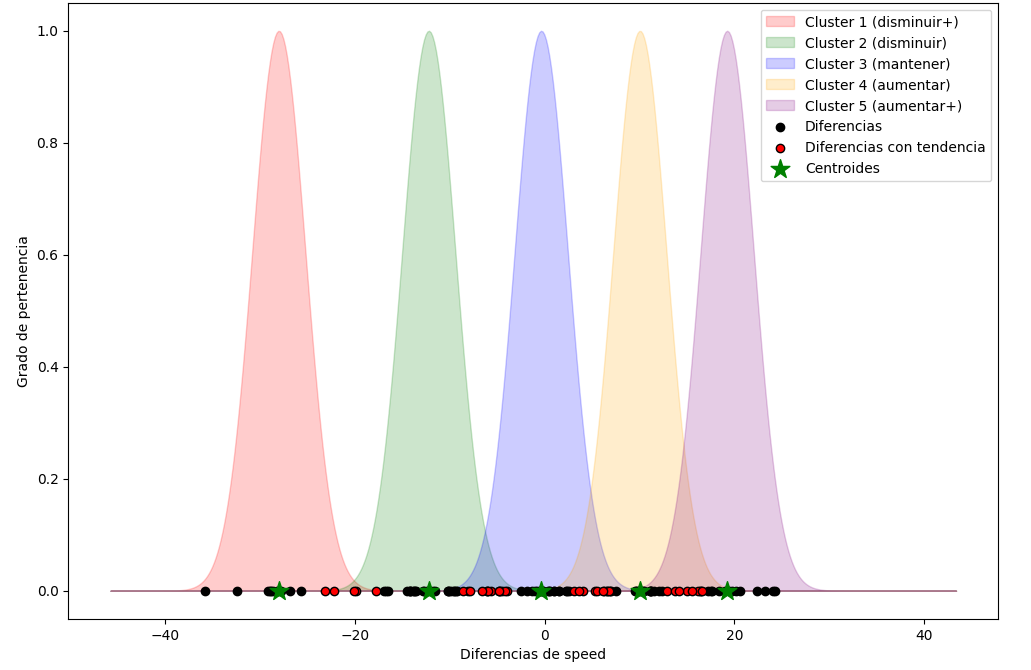
\includegraphics[width=1\linewidth]{./figs/herramientas/desarrollo/etiquetas_difusas.png}
	\caption[Diagrama de dispersión con conjuntos difusos para la variable ``speed'']{Diagrama de dispersión con conjuntos difusos para la variable ``speed''}
    \label{fig:etiquetas_difusas}
\end{figure}


Finalmente, se añadió la información del etiquetado al modelo de clases en Rust, utilizando enums con métodos de creación e incremento, como se muestra en la \autoref{fig:diagrama_clases_etiquetas}.

\begin{figure}[H]
	\centering
	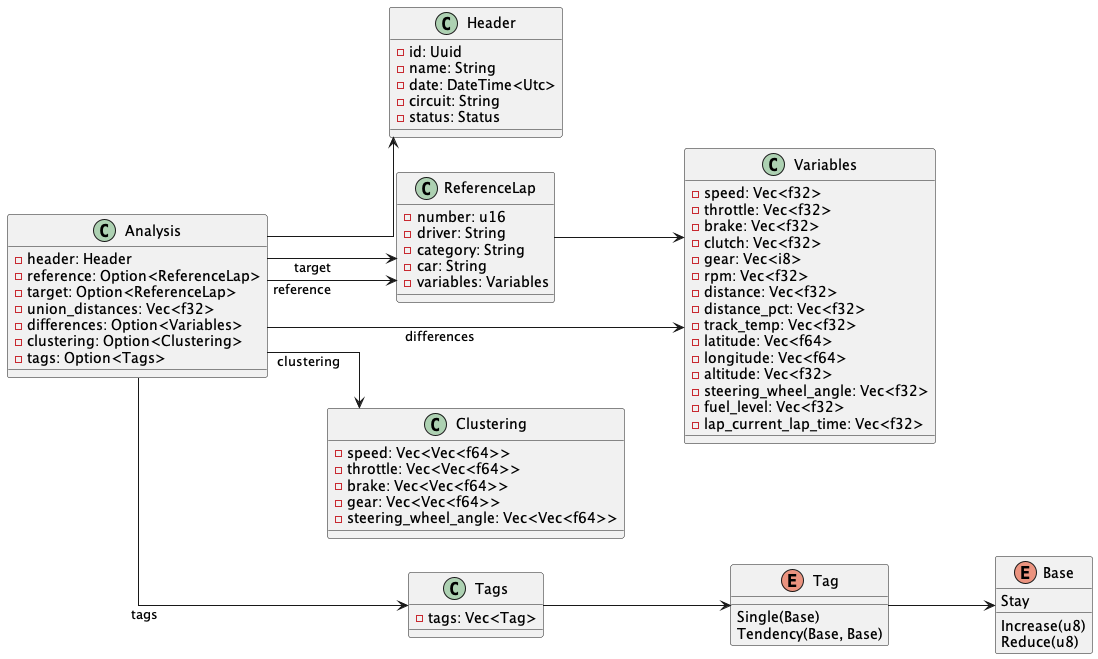
\includegraphics[width=1\linewidth]{./figs/herramientas/desarrollo/diagrama_clases_etiquetas.png}
	\caption[Diagrama de clases con etiquetas asignadas]{Diagrama de clases con etiquetas asignadas}
    \label{fig:diagrama_clases_etiquetas}
\end{figure}


\newpage

\section{Hito 5: Desarrollo de aplicación web \textit{(SO5)}}

El desarrollo de la aplicación web se centró en la creación de una plataforma accesible y funcional para gestionar y analizar los datos de telemetría extraídos. Este hito incluyó la implementación de varias características clave que permitieron a los usuarios subir y gestionar ficheros de telemetría, realizar análisis comparativos entre diferentes vueltas y visualizar los resultados de manera intuitiva. A continuación se presenta la tabla resumen de este hito:

\begin{table}[H]
\centering
\begin{tabular}{|l|c|}
\hline
\textbf{Título} & Desarrollo de Aplicación Web \\ \hline
\textbf{Código} & \textit{SO5} \\ \hline
\textbf{Historias de Usuario} & 4 \\ \hline
\textbf{Sprints} & 29-34 \\ \hline
\end{tabular}
\caption{Resumen de la sección: Desarrollo de Aplicación Web}
\label{tab:desarrollo_aplicacion_web}
\end{table}

% Párrafo introductorio a las historias de usuario
A continuación se detallan las historias de usuario que conformaron este hito, enfocadas en la creación y mejora de la aplicación web para gestionar y analizar los datos de telemetría de manera eficiente.

% Historia de Usuario 1
\subsection{Diseño de la arquitectura de la aplicación web}
\begin{table}[H]
\centering
\begin{tabular}{|l|p{10cm}|}
\hline
\multicolumn{2}{|c|}{\textbf{Historia de Usuario 12}} \\ \hline
\textbf{Nombre:} & Diseño de la arquitectura de la aplicación web \\ \hline
\textbf{Descripción:} & Como cliente del proyecto, quiero un diseño robusto de la arquitectura de la aplicación web, que garantice escalabilidad, seguridad y facilidad de mantenimiento, para asegurar un desempeño óptimo y una experiencia de usuario eficiente. \\ \hline
\textbf{Prioridad:} & P1 \\ \hline
\textbf{Talla:} & L \\ \hline
\textbf{Sprints:} & 29 \\ \hline
\end{tabular}
\caption{Historia de Usuario 12}
\label{tab:diseno_arquitectura_web}
\end{table}

En esta historia de usuario se diseñó la arquitectura de la aplicación web, asegurando escalabilidad, seguridad y facilidad de mantenimiento, para ofrecer un desempeño óptimo y una experiencia de usuario eficiente. A continuación, se presenta una descripción detallada de cómo se estructuró y construyó la arquitectura, tanto para el \textit{backend} como para el \textit{frontend}.

\subsubsection*{Backend}
\begin{itemize}
    \item \textbf{Estructura}: se organizó siguiendo los principios de \ac{ddd}, permitiendo una clara separación de responsabilidades y facilitando la reutilización de componentes. La organización principal es la siguiente:
    \begin{itemize}
        \item \textbf{api}: Maneja la infraestructura de la aplicación, ensamblando componentes, controladores y suscriptores.
        \item \textbf{ibt\_extractor}: Gestiona la extracción y conversión de datos de telemetría.
        \item \textbf{main.rs}: Punto de entrada principal de la aplicación \textit{backend}.
        \item \textbf{backend-config.yaml}: Archivo de configuración que incluye parámetros específicos para la ejecución del \textit{backend}.
    \end{itemize}
    \item \textbf{Axum y Green Threads}: se eligió \textit{Axum} \cite{axum_github} debido a su rendimiento y capacidad de manejo multihilo, desarrollado por los creadores de \textit{Tokio} \cite{tokio}, librería de referencia para programación concurrente en Rust (\autoref{fig:rust}). \textit{Axum} se destacó por su robustez y eficiencia en la gestión de solicitudes concurrentes, esencial para asegurar un desempeño óptimo en el procesamiento de datos de telemetría. Se utilizaron \textit{green threads} \cite{green_thread} de Rust para crear un servidor multihilo, permitiendo gestionar múltiples hilos de ejecución de manera eficiente. Los \textit{green threads} son una abstracción de hilos de bajo nivel que permiten un manejo más eficiente de las tareas concurrentes.
        \begin{figure}[H]
        	\centering
        	
\includegraphics[width=0.3\linewidth]{./figs/herramientas/desarrollo/rust.png}
        	\caption[Logotipo de Rust]{Logotipo de Rust}
            \label{fig:rust}
        \end{figure}
    \item \textbf{Controladores y Suscriptores de Eventos}: La capa de infraestructura del \textit{backend} se diseñó para implementar los servicios expuestos por la capa de aplicación de dos formas:
    \begin{itemize}
        \item \textbf{Controladores}: Implementan las \ac{api} \ac{rest} clásicas, permitiendo la comunicación entre el cliente y el servidor a través de \ac{http}. Estos controladores gestionan solicitudes, procesan datos y devuelven respuestas adecuadas.
        \item \textbf{Suscriptores}: Servicios que se ejecutan de manera reactiva ante eventos del sistema. Estos suscriptores escuchan eventos específicos y desencadenan acciones en respuesta, permitiendo una arquitectura más flexible y reactiva.
    \end{itemize}
    \item \textbf{Arquitectura Hexagonal}: Los elementos de la arquitectura hexagonal \cite{hexagonal_architecture} se definieron mediante repositorios y otros puertos como interfaces de dominio. La arquitectura hexagonal, también conocida como Arquitectura de Puertos y Adaptadores, promueve la separación de la lógica de negocio del resto del sistema, facilitando el mantenimiento y la escalabilidad. Esta arquitectura se complementa perfectamente con los principios de \ac{ddd}, que enfoca el diseño del software en el dominio central de la aplicación y su lógica de negocio.

    En esta arquitectura, los puertos actúan como interfaces que definen las operaciones disponibles para el dominio. Los adaptadores implementan estos puertos y permiten que la lógica de negocio interactúe con servicios externos, bases de datos y otros sistemas. Este enfoque asegura que los componentes del dominio no estén acoplados a la infraestructura técnica, como bases de datos o servicios externos.
    
    En esta implementación:
    \begin{itemize}
        \item \textbf{Repositorios}: Definidos como interfaces en el dominio, permiten acceder a los datos de una manera desacoplada. Las implementaciones específicas de estos repositorios se encuentran en la capa de infraestructura, garantizando que el dominio no dependa de detalles específicos de almacenamiento.
        \item \textbf{Servicios externos}: Se accede a través de interfaces definidas en el dominio. Estas interfaces son implementadas por adaptadores en la capa de infraestructura, permitiendo cambiar fácilmente los servicios externos sin afectar la lógica de negocio.
    \end{itemize}
    
    Este diseño permitió una clara separación de responsabilidades, facilitando pruebas unitarias, mantenimiento y escalabilidad de la aplicación.
\end{itemize}

\subsubsection*{Frontend}
\begin{itemize}
        \item \textbf{Estructura}: se eligió el framework \textit{Yew} \cite{yew}, que utiliza una arquitectura similar a \textit{React} \cite{react} y \textit{Elm} \cite{elm_components}. \textit{Yew} permite estructurar la aplicación con componentes reutilizables, facilitando el desarrollo y mantenimiento de la interfaz de usuario. La organización principal es la siguiente:
    \begin{itemize}
        \item \textbf{src}: Contiene el código fuente del \textit{frontend}, dividido en:
        \begin{itemize}
            \item \textbf{infrastructure}: Maneja componentes, repositorios y configuración del \textit{frontend}.
            \item \textbf{main.rs}: Punto de entrada principal de la aplicación \textit{frontend}.
        \end{itemize}
        \item \textbf{assets}: Archivos estáticos como \ac{css}, imágenes y scripts.
        \item \textbf{frontend-config.yaml}: Archivo de configuración que incluye parámetros específicos para la ejecución del \textit{frontend}.
    \end{itemize}
    \item \textbf{Componentes Reutilizables en Yew}:\textit{Yew} (\autoref{fig:yew}) permite la creación de componentes reutilizables, lo que facilita el desarrollo y mantenimiento de la interfaz de usuario. Los componentes en \textit{Yew} son unidades independientes de funcionalidad que se pueden combinar para construir interfaces complejas de manera modular. Esto proporciona varios beneficios:
    \begin{itemize}
        \item \textbf{Reutilización}: Los componentes se pueden reutilizar en diferentes partes de la aplicación, reduciendo la duplicación de código y facilitando el mantenimiento.
        \item \textbf{Modularidad}: La aplicación se puede dividir en componentes más pequeños y manejables, lo que mejora la organización del código y facilita la comprensión y el desarrollo.
        \item \textbf{Facilidad de Mantenimiento}: Los cambios en la lógica de un componente no afectan a otros componentes, lo que reduce el riesgo de errores y facilita la actualización de la aplicación.
        \begin{figure}[H]
        	\centering
        	
\includegraphics[width=0.3\linewidth]{./figs/herramientas/desarrollo/yew.png}
        	\caption[Logotipo de Yew]{Logotipo de Yew}
            \label{fig:yew}
        \end{figure}
    \end{itemize}
    \item \textbf{Integración con el Backend}: El \textit{frontend} implementa los repositorios contra la \ac{api} \ac{rest} del \textit{backend}, mientras que el \textit{backend} lo hace contra MongoDB \cite{mongodb}. Ambos serializan y deserializan los objetos de la misma manera, aprovechando todos los elementos desarrollados en los hitos anteriores desde ambos lados. Esto asegura que cualquier cambio en la lógica de negocio se refleje tanto en el cliente como en el servidor de manera uniforme.
    \item \textbf{WebAssembly}: Se utilizó \ac{wasm} (\autoref{fig:wasm}) para permitir la ejecución de código Rust tanto en el \textit{backend} como en el \textit{frontend}, facilitando la reutilización de la lógica de negocio y mejorando la eficiencia del desarrollo. \ac{wasm} es un estándar que permite ejecutar código de bajo nivel en los navegadores web, proporcionando un rendimiento cercano al nativo. Esto permite que lenguajes como Rust, conocidos por su seguridad y eficiencia, se utilicen en el desarrollo de aplicaciones web complejas. Al utilizar \ac{wasm}, se garantiza que la lógica de negocio implementada en Rust se pueda ejecutar de manera eficiente en el navegador, proporcionando una experiencia de usuario fluida y reduciendo la carga de trabajo del \textit{backend}.
        \begin{figure}[H]
        \centering
        
\includegraphics[width=0.3\linewidth]{./figs/herramientas/desarrollo/wasm.png}
        \caption[Logotipo de \ac{wasm}]{Logotipo de \ac{wasm}}
        \label{fig:wasm}
        \end{figure}
\end{itemize}

\subsubsection*{Beneficios de la Arquitectura Diseñada}
La arquitectura diseñada garantizó:
\begin{itemize}
    \item \textbf{Escalabilidad}: La estructura modular y el uso de tecnologías eficientes permitieron el crecimiento y adaptación de la aplicación según las necesidades.
    \item \textbf{Seguridad}: La configuración adecuada y el uso de tecnologías robustas aseguraron la protección de los datos y las operaciones del sistema.
    \item \textbf{Facilidad de Mantenimiento}: La separación clara de responsabilidades y la reutilización de componentes facilitaron la gestión y actualización de la aplicación.
    \item \textbf{Desempeño Óptimo}: La selección cuidadosa de tecnologías y la implementación eficiente aseguraron un rendimiento excelente de la aplicación.
    \item \textbf{Experiencia de Usuario Eficiente}: La interfaz intuitiva y la rapidez de respuesta proporcionaron una experiencia de usuario satisfactoria y efectiva.
\end{itemize}

% Historia de Usuario 2
\subsection{Gestión de Ficheros de Telemetría}
\begin{table}[H]
\centering
\begin{tabular}{|l|p{10cm}|}
\hline
\multicolumn{2}{|c|}{\textbf{Historia de Usuario 13}} \\ \hline
\textbf{Nombre:} & Gestión de Ficheros de Telemetría \\ \hline
\textbf{Descripción:} & Como usuario, quiero poder subir ficheros de telemetría, visualizar las vueltas contenidas en ellos, y tener la capacidad de borrar ficheros completos o vueltas individuales, para gestionar mis datos de manera eficiente. \\ \hline
\textbf{Prioridad:} & P1 \\ \hline
\textbf{Talla:} & M \\ \hline
\textbf{Sprints:} & 30 \\ \hline
\end{tabular}
\caption{Historia de Usuario 13}
\label{tab:gestion_ficheros_telemetria}
\end{table}

\subsubsection*{Backend}

Para la implementación de la funcionalidad de gestión de ficheros de telemetría en el \textit{backend}, se diseñaron e implementaron los servicios necesarios dentro de la capa de aplicación. Se creó el módulo \texttt{ibt\_extractor}, que se encarga de recibir un objeto que implementa los traits \texttt{Read} y \texttt{Seek} y devuelve una estructura \texttt{IBTFile} con los datos extraídos. Dado que este servicio utiliza intensivamente la entrada y salida, se implementó como un suscriptor de eventos. Concretamente, este servicio escucha el evento \texttt{FileUploaded}, que se emite cuando se han transferido todos los bytes del fichero \texttt{ibt} desde el equipo del cliente. La extracción se ejecuta en un hilo separado, devolviendo un código \texttt{CONTINUE} de HTTP para evitar el bloqueo del cliente.

Se creó una estructura \texttt{File} para representar un fichero de telemetría dentro del dominio, independiente del sistema \textit{iRacing}. Esta estructura contiene atributos como el \texttt{SHA256} del fichero, su nombre, su estado y la fecha de creación. Cuando un usuario sube un fichero, se crea automáticamente un objeto \texttt{File} en el sistema cuyo \texttt{id} corresponde al \texttt{SHA256} del fichero \texttt{ibt} (para evitar redundancia de información) y se inicializa con el estado \texttt{Accepted}. Al completarse la extracción, se emite un evento \texttt{IbtExtracted}, al que está suscrito el servicio \texttt{validate} del módulo \texttt{file}. Este servicio cambia el estado del fichero de \texttt{Accepted} a \texttt{Success}. En caso de error durante la extracción, otro servicio de la capa de aplicación del dominio \texttt{File}, denominado \texttt{mark\_as\_error}, escucha el evento y marca el fichero como erróneo, junto con un mensaje explicativo de la razón. En la \autoref{fig:seq_file_upload} se muestra el diagrama de secuencia de lo anterior.

\begin{figure}[H]
\centering
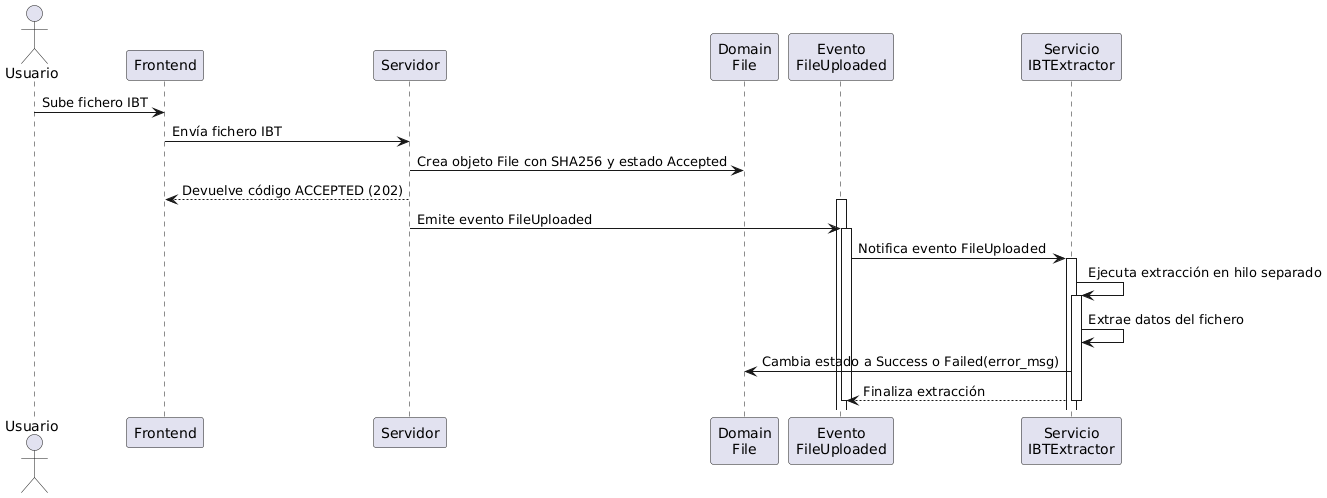
\includegraphics[width=1\linewidth]{./figs/herramientas/desarrollo/seq_file_upload.png}
\caption[Diagrama de secuencia de subida de un fichero]{Diagrama de secuencia de subida de un fichero}
\label{fig:seq_file_upload}
\end{figure}

Cuando un fichero se marca como \texttt{Success}, se emite otro evento que se encarga de almacenar todas las vueltas (\texttt{Laps}) contenidas en el fichero extraído en el sistema. Además, si un \texttt{File} se elimina, se emite un evento \texttt{FileDeleted}, al cual está suscrito un servicio del módulo \texttt{Lap}, que elimina del sistema todas las vueltas (\texttt{Laps}) cuyo \texttt{file\_id} corresponde al fichero eliminado. Se puede ver este funcionamiento en la \autoref{fig:seq_file_store_and_delete_laps}.

\begin{figure}[H]
\centering
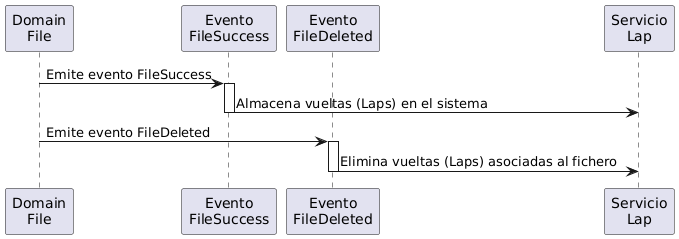
\includegraphics[width=1\linewidth]{./figs/herramientas/desarrollo/seq_file_store_and_delete_laps.png}
\caption[Diagrama de secuencia de guardado y borrado de vueltas]{Diagrama de secuencia de guardado y borrado de vueltas}
\label{fig:seq_file_store_and_delete_laps}
\end{figure}

El módulo \texttt{lap} se encarga de gestionar las vueltas (\texttt{Laps}) extraídas de los ficheros de telemetría. Este módulo incluye servicios para crear, eliminar y encontrar vueltas, así como para obtener los encabezados de las vueltas. En el dominio, se definen las estructuras de las vueltas, incluyendo los encabezados y las variables asociadas a cada vuelta. Los repositorios se utilizan para abstraer el acceso a los datos y facilitar la persistencia y recuperación de las vueltas en el sistema.

\subsubsection*{Frontend}
El componente de subida de ficheros permite al usuario seleccionar un archivo desde su dispositivo y enviar una petición al \textit{backend} para subirlo. Dado que el comportamiento predeterminado de un componente \texttt{form} en \ac{html} es redirigir a la página especificada en el atributo \texttt{action} una vez que la petición se completa, se tuvo que manejar manualmente la subida multipart para mantener la interfaz de usuario sin interrupciones. Esto se logró implementando funciones asíncronas que procesan la subida de archivos y gestionan las respuestas del servidor sin bloquear la interfaz.


En la pantalla de \textit{Files} (\autoref{fig:front_file}), además del componente de subida, se incluye una lista de los ficheros de telemetría almacenados en el sistema. Cada entrada de la lista muestra el nombre del fichero y ofrece dos opciones: 
\begin{itemize}
    \item \textbf{Borrar Fichero}: Permite al usuario eliminar un fichero del sistema. Al seleccionar esta opción, se emite el evento \texttt{FileDeleted}, desencadenando la eliminación de todas las vueltas (\texttt{Laps}) asociadas a dicho fichero.
    \item \textbf{Visualizar Vueltas}: Proporciona al usuario la capacidad de ver todas las vueltas contenidas en el fichero seleccionado. Esto se realiza mediante un botón que redirige a una pantalla donde se detallan todas las vueltas asociadas al fichero.
\end{itemize}

\begin{figure}[H]
\centering
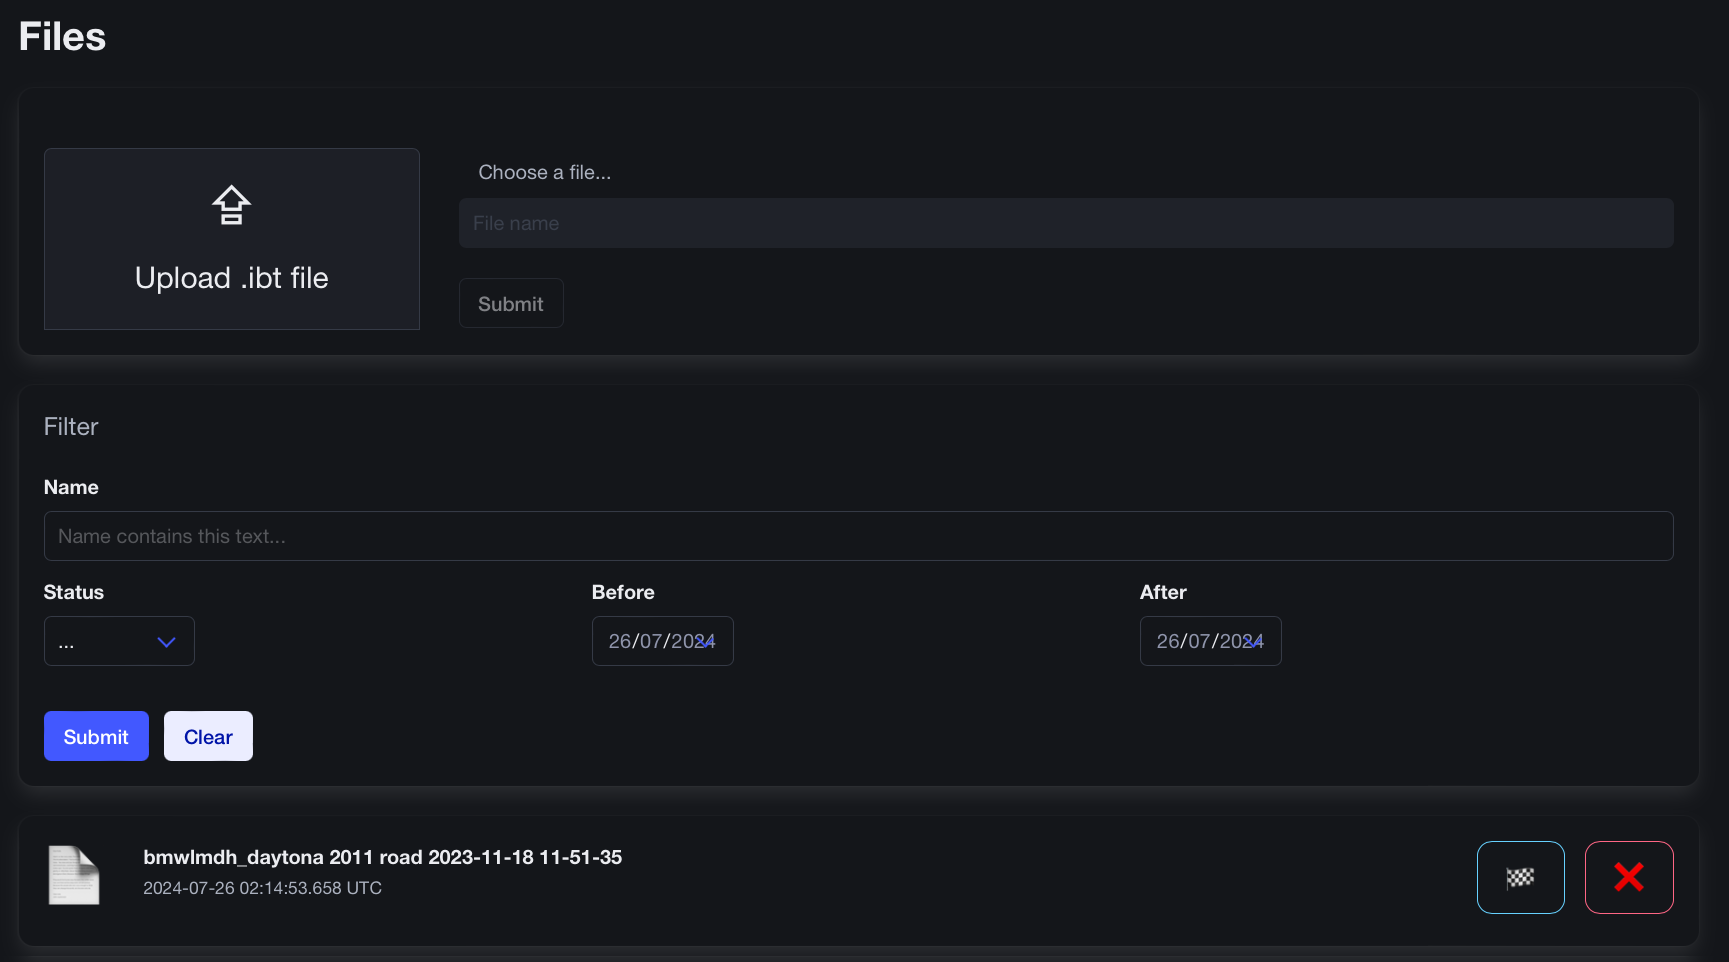
\includegraphics[width=1\linewidth]{./figs/herramientas/desarrollo/front_file.png}
\caption[Pantalla de Files]{Pantalla de Files}
\label{fig:front_file}
\end{figure}

En la \autoref{fig:front_file_accepted} se muestra el icono de fichero aceptado, que indica que el archivo de telemetría ha sido correctamente recibido por el sistema y está pendiente de procesamiento.

\begin{figure}[H]
\centering
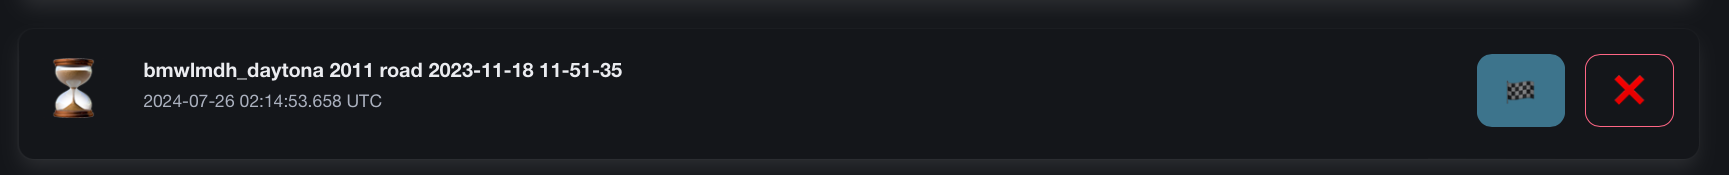
\includegraphics[width=1\linewidth]{./figs/herramientas/desarrollo/front_file_accepted.png}
\caption[Fichero en estado Accepted]{Fichero en estado Accepted}
\label{fig:front_file_accepted}
\end{figure}

En la \autoref{fig:front_file_success} se presenta el icono de fichero satisfactorio, señalando que el archivo ha sido procesado con éxito y sus datos han sido extraídos y almacenados correctamente.

\begin{figure}[H]
\centering
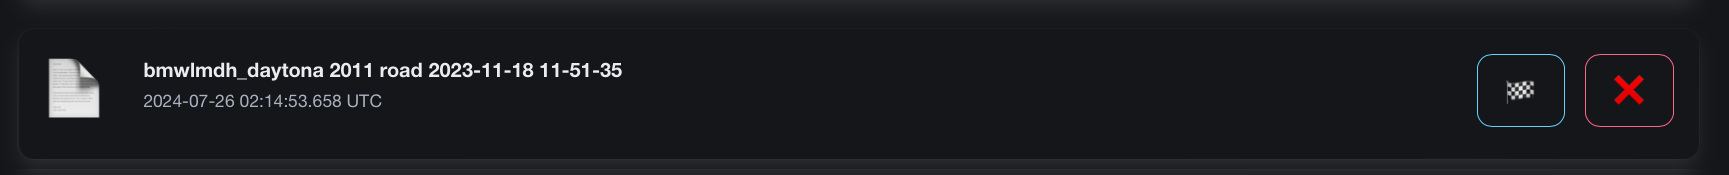
\includegraphics[width=1\linewidth]{./figs/herramientas/desarrollo/front_file_success.png}
\caption[Fichero en estado Success]{Fichero en estado Success}
\label{fig:front_file_success}
\end{figure}

% Historia de Usuario 3
\subsection{Realización de análisis comparativo entre vueltas}
\begin{table}[H]
\centering
\begin{tabular}{|l|p{10cm}|}
\hline
\multicolumn{2}{|c|}{\textbf{Historia de Usuario 14}} \\ \hline
\textbf{Nombre:} & Realización de análisis comparativo entre vueltas \\ \hline
\textbf{Descripción:} & Como usuario, quiero poder realizar análisis comparativos entre dos vueltas seleccionadas, pudiendo filtrar por diferentes atributos. \\ \hline
\textbf{Prioridad:} & P1 \\ \hline
\textbf{Talla:} & S \\ \hline
\textbf{Sprints:} & 30-31 \\ \hline
\end{tabular}
\caption{Historia de Usuario 14}
\label{tab:analisis_comparativo_vueltas}
\end{table}

\subsubsection*{Backend}

El módulo \texttt{Analysis} encapsuló todos los servicios necesarios para realizar un análisis comparativo entre dos vueltas. El proceso de creación de un análisis comienza con la recepción de un identificador (ID), un nombre, una fecha, un ID de la vuelta de referencia y un ID de la vuelta a comparar.

El módulo de análisis llama al servicio de búsqueda de vueltas del módulo \texttt{Lap} para comprobar la existencia de ambas vueltas. Además, verifica que ambas vueltas pertenezcan al mismo circuito para garantizar la validez de la comparación. Una vez confirmadas estas condiciones, se crea una instancia de la estructura \texttt{Analysis} y se emite el evento \texttt{AnalysisCreated}. El \texttt{Analysis} comienza con estado Accepted

En este punto, se devuelve un código \ac{http} 202 (Accepted) al cliente, con el fin de evitar tiempos de bloqueo en la interfaz de usuario. El servicio \texttt{analyze} del módulo \texttt{Analysis}, implementado como un suscriptor, escucha este evento y realiza el análisis en segundo plano. En la \autoref{fig:seq_create_analysis} se muestra el diagrama de secuencia que representa lo anterior.

\begin{figure}[H]
\centering
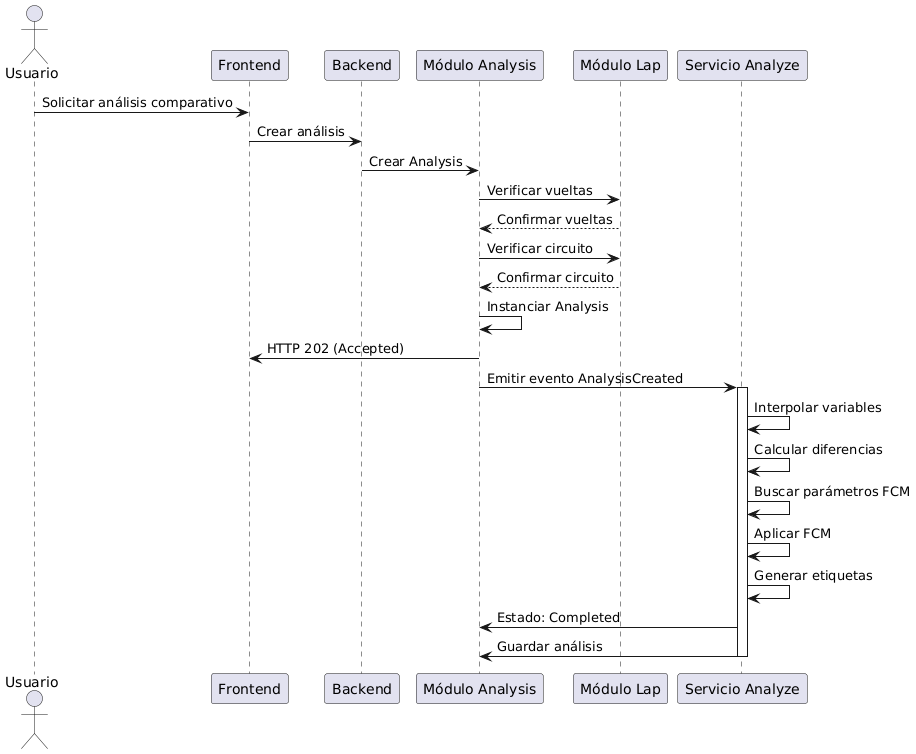
\includegraphics[width=0.6\linewidth]{./figs/herramientas/desarrollo/seq_create_analysis.png}
\caption[Diagrama de secuencia de creación de un Análisis]{Diagrama de secuencia de creación de un Análisis}
\label{fig:seq_create_analysis}
\end{figure}

El análisis comienza interpolando los valores de las variables de la vuelta de referencia y la vuelta a comparar en función de la unión de las distancias. Posteriormente, calcula el vector de diferencias, ejecuta la búsqueda de parámetros del algoritmo \ac{fcm}, aplica \ac{fcm} con los parámetros óptimos y genera las etiquetas correspondientes. Finalmente, la instancia de \texttt{Analysis} pasa del estado \texttt{Accepted} a \texttt{Completed}.

Una vez completado el análisis, toda la información generada se guardó en el sistema, y el análisis quedó disponible para su consulta posterior.

\subsubsection*{Frontend}

Para el desarrollo del frontend, se implementó una pantalla dedicada a la gestión de análisis comparativos entre vueltas de telemetría. Esta pantalla muestra las vueltas disponibles en el sistema y permite al usuario seleccionar dos de ellas para realizar un análisis. La funcionalidad principal de esta pantalla se centró en la selección de vueltas y la solicitud de creación de análisis comparativos.

Primero, se diseñó e implementó una lista de vueltas disponibles en el sistema. Esta lista proporciona información detallada de cada vuelta, permitiendo al usuario identificar rápidamente las vueltas que desea comparar. Para facilitar la búsqueda de vueltas específicas, se implementó una funcionalidad de filtrado. Este filtrado permite al usuario buscar vueltas que cumplan determinados criterios, tales como el nombre del circuito, el nombre del piloto, o el tiempo de la vuelta (\autoref{fig:front_analysis_list}).

\begin{figure}[H]
\centering
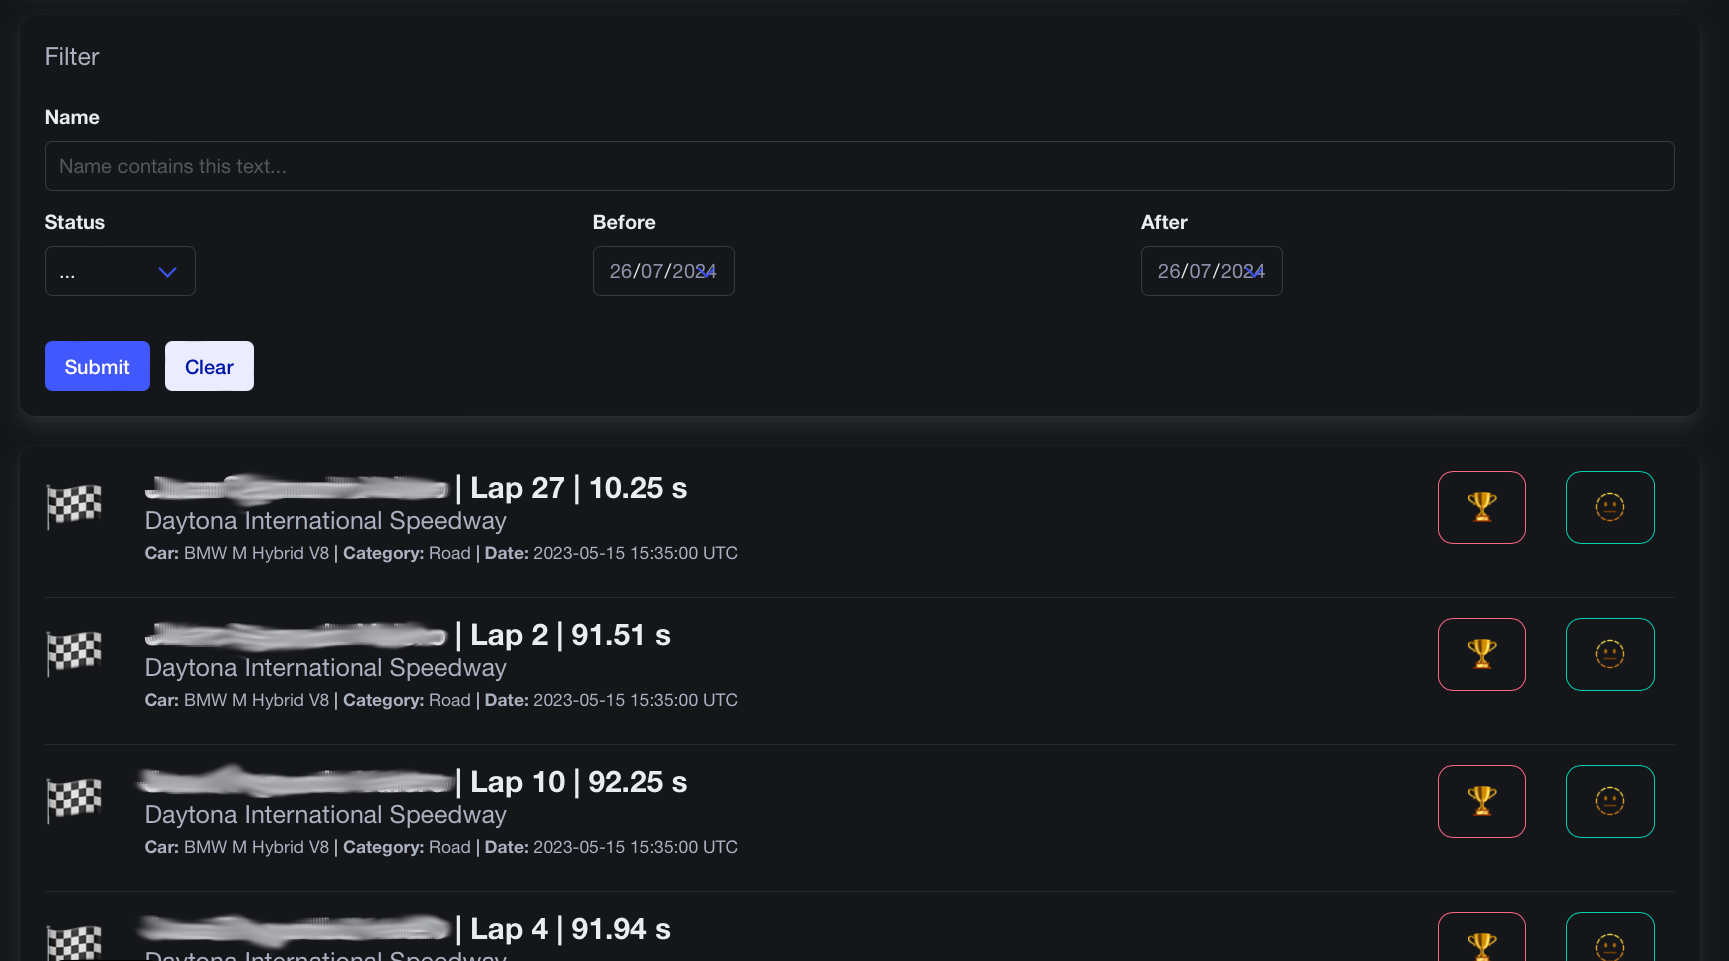
\includegraphics[width=0.6\linewidth]{./figs/herramientas/desarrollo/front_analysis_list.png}
\caption[Listado de vueltas en un Análisis]{Listado de vueltas en un Análisis}
\label{fig:front_analysis_list}
\end{figure}

Cada elemento de la lista de vueltas incluye dos botones al final: uno para seleccionar la vuelta como vuelta de referencia y otro para seleccionarla como vuelta a comparar (\autoref{fig:front_analysis_btn}). Al pulsar el botón de vuelta de referencia, la vuelta seleccionada se añade como la vuelta de referencia para el análisis. De manera similar, al pulsar el botón de vuelta a comparar, la vuelta seleccionada se añade como la vuelta a comparar para el análisis. Esta implementación permite al usuario seleccionar fácilmente las vueltas que desea comparar sin necesidad de cambiar de pantalla o realizar acciones adicionales complicadas.

\begin{figure}[H]
\centering

\includegraphics[width=0.3\linewidth]{./figs/herramientas/desarrollo/front_analysis_btn.png}
\caption[Botones de las vueltas en un Análisis]{Botones de las vueltas en un Análisis}
\label{fig:front_analysis_btn}
\end{figure}

Una vez que el usuario ha seleccionado las vueltas de referencia y a comparar, puede proceder a completar la creación del análisis en el componente de selección de vueltas (\autoref{fig:front_analysis_creator}). El componente de selección de vueltas permite al usuario ingresar un nombre y una fecha para el análisis, asegurando que los detalles del análisis sean claros y fácilmente identificables.

\begin{figure}[H]
\centering
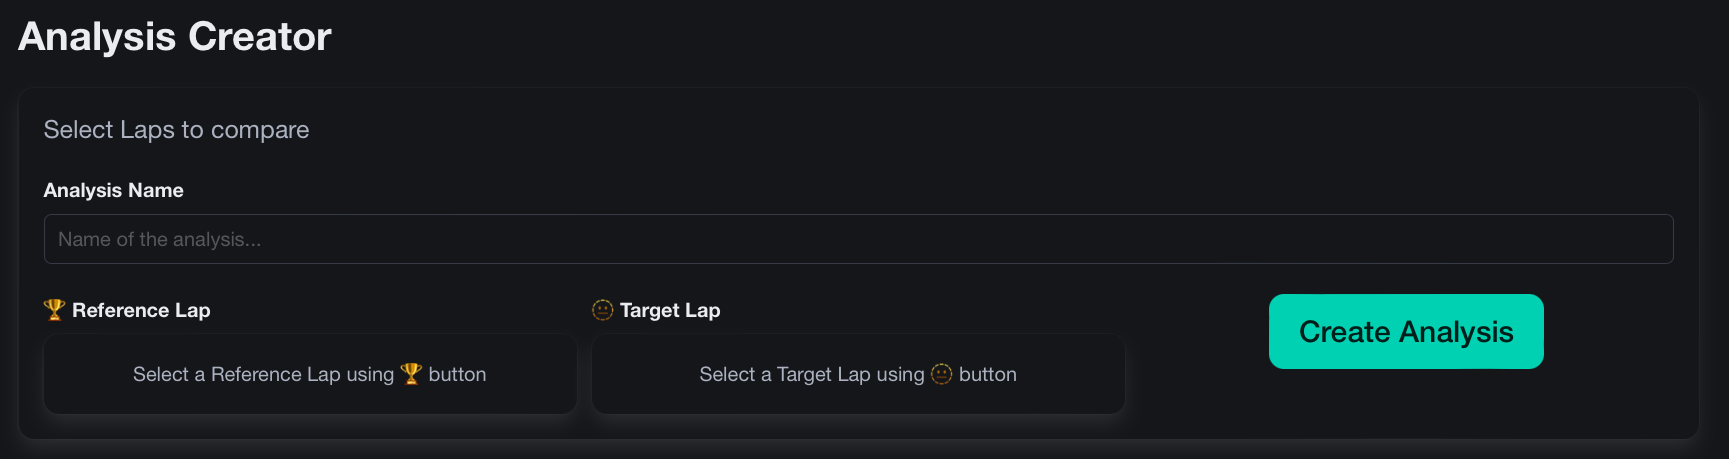
\includegraphics[width=0.6\linewidth]{./figs/herramientas/desarrollo/front_analysis_creator.png}
\caption[Selector de vueltas en un Análisis]{Selector de vueltas en un Análisis}
\label{fig:front_analysis_creator}
\end{figure}

Finalmente, al pulsar el botón de enviar, el frontend envía una solicitud al backend para crear el análisis comparativo entre las dos vueltas seleccionadas. Esta solicitud se gestiona de manera asíncrona, asegurando que la interfaz de usuario permanezca receptiva y evitando tiempos de espera prolongados para el usuario.

La pantalla de gestión de análisis comparativos se diseñó para proporcionar una experiencia de usuario intuitiva y eficiente, permitiendo a los usuarios realizar análisis detallados de su rendimiento de manera rápida y sencilla.

% Historia de Usuario 4
\subsection{Visualización de resultados del análisis en un cuadro de mandos}
\begin{table}[H]
\centering
\begin{tabular}{|l|p{10cm}|}
\hline
\multicolumn{2}{|c|}{\textbf{Historia de Usuario 15}} \\ \hline
\textbf{Nombre:} & Visualización de resultados del análisis en un cuadro de mandos \\ \hline
\textbf{Descripción:} & Como usuario, quiero poder visualizar los resultados del análisis de telemetría en un cuadro de mandos interactivo para facilitar la interpretación y toma de decisiones basadas en los datos. \\ \hline
\textbf{Prioridad:} & P1 \\ \hline
\textbf{Talla:} & M \\ \hline
\textbf{Sprints:} & 32-34 \\ \hline
\end{tabular}
\caption{Historia de Usuario 15}
\label{tab:visualizacion_resultados_dashboard}
\end{table}

Para la implementación de la funcionalidad de visualización de resultados del análisis de telemetría en un cuadro de mandos interactivo, se desarrolló un componente \textit{Yew} compuesto por varios sub-componentes. Esta historia de usuario se centró exclusivamente en el \textit{frontend}, dado que ya existían todos los componentes necesarios en el \textit{backend}.

El cuadro de mandos se diseñó para mostrar los diagramas de dispersión de las variables más representativas según el consultor del proyecto. Estas variables son velocidad, porcentaje del pedal de aceleración pisado, porcentaje del pedal de freno pisado, marcha y ángulo de giro del volante. Estas son las mismas variables que utilizan la mayoría de los sistemas comerciales.

Para cada una de estas cinco variables, se mostró un diagrama de dispersión. En estos diagramas, el eje x representa la distancia o el punto del circuito donde se encuentra el vehículo, medido en metros. Los ejes y se dividieron en dos: uno que muestra los valores de la variable para ambas vueltas y otro que presenta el valor de la diferencia en una escala diferente. Se apilaron los diagramas de dispersión de manera que se puedan observar de forma conjunta, tal y como se muestra en la \autoref{fig:dashboard}. Además, se sincronizó el cursor de todas las gráficas para que se moviera simultáneamente, aprovechando que el eje x es la distancia para todas las variables. Esta sincronización facilita la comparación en tiempo real de las variables a lo largo del circuito.

Otro componente esencial del cuadro de mandos es un \textit{canvas \ac{html}} con el circuito dibujado. En este \textit{canvas \ac{html}}, se añadió un puntero que, al moverse, también mueve el cursor de los diagramas de dispersión al punto correspondiente. Para lograr esta interacción, se utilizaron enlaces entre JavaScript y Rust mediante \ac{wasm}.

Debajo del circuito, se implementaron unos botones de radio que permiten seleccionar una de las variables analizadas. Al seleccionar una variable, el circuito pinta cada uno de sus puntos de un color específico en función de la agrupación a la que pertenece y el grado de pertenencia. Esta visualización facilita la identificación de los puntos donde hay mayores diferencias en la variable seleccionada, proporcionando una vista clara y detallada del rendimiento en el circuito.

Por último, debajo del selector de variables, se añadió un panel que muestra, en lenguaje natural, una acción recomendada en función de la etiqueta lingüística asignada. Esta funcionalidad ofrece una guía clara y directa sobre las acciones a tomar para mejorar el rendimiento basado en el análisis de telemetría. El cudro de mandos completo se muestra en la \autoref{fig:dashboard}.
\begin{figure}[H]
\centering
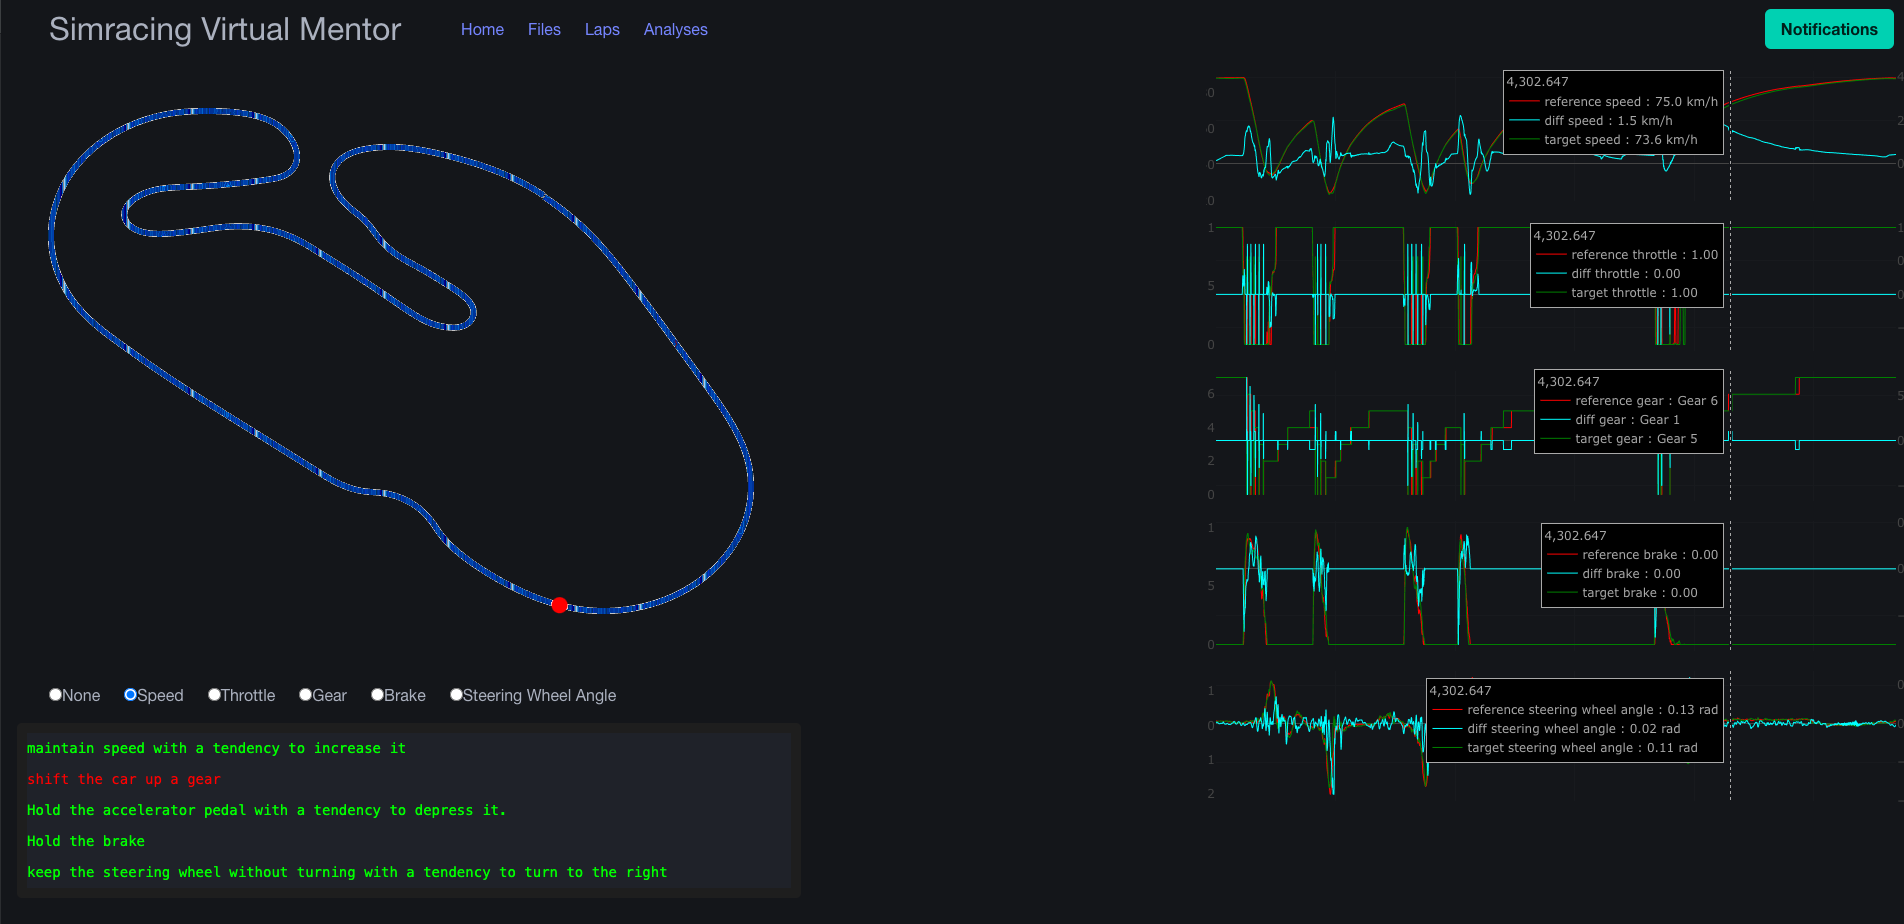
\includegraphics[width=1\linewidth]{./figs/herramientas/desarrollo/svm.png}
\caption[Cuadro de Mandos]{Cuadro de Mandos}
\label{fig:dashboard}
\end{figure}

La integración de estos componentes en un cuadro de mandos interactivo ha permitido una visualización detallada y comprensible de los datos de telemetría, facilitando la interpretación y la toma de decisiones basadas en los datos analizados.
\chapter{Conclusiones}
\label{cap:Conclusiones}

En este capítulo se presentan las conclusiones del trabajo realizado, evaluando el grado de cumplimiento de los objetivos planteados y destacando las competencias adquiridas a lo largo del desarrollo del proyecto. Asimismo, se discutirán los trabajos derivados y futuros que pueden surgir a partir de este proyecto y se ofrecerá una valoración personal sobre las lecciones aprendidas y la experiencia obtenida.


\section{Objetivos alcanzados}

El objetivo principal del \ac{tfg} era diseñar y desarrollar un entrenador virtual de código abierto capaz de interpretar archivos de telemetría del software iRacing. Este entrenador debía proporcionar un análisis detallado, permitiendo la visualización de métricas comparativas entre dos vueltas en un circuito, y ofrecer recomendaciones de mejora de la conducción en lenguaje natural. Este objetivo se ha cumplido satisfactoriamente, desarrollando una herramienta robusta y eficiente que facilita la comprensión y aplicación de las mejoras por parte de los pilotos, contribuyendo a su rendimiento y desarrollo en el Simracing.

Para alcanzar este objetivo general, se plantearon los siguientes objetivos específicos, todos los cuales han sido alcanzados:

\subsection{Adquirir y procesar datos de telemetría}
\begin{itemize}
    \item Se investigó cómo se adquieren y transfieren los ficheros de telemetría .ibt de iRacing y se consiguió una muestra.
    \item Se estudió el formato de telemetría .ibt de iRacing.
    \item Se desarrolló un módulo para la lectura y decodificación de archivos de telemetría en formato .ibt.
\end{itemize}

\subsection{Fijar las métricas de comparación}
\begin{itemize}
    \item Se identificaron y seleccionaron las variables de telemetría relevantes para su posterior comparación.
    \item Se desarrolló un modelo que define y permite comparar los datos de telemetría.
\end{itemize}

\subsection{Comparar datos de telemetría y aplicar aprendizaje no supervisado para clasificar diferencias}
\begin{itemize}
    \item Se implementaron métodos para la comparación de datos de telemetría.
    \item Se aplicaron técnicas de aprendizaje no supervisado para clasificar las diferencias observadas.
\end{itemize}

\subsection{Construir el conjunto de sugerencias con una respuesta en lenguaje natural}
\begin{itemize}
    \item Se desarrolló un método sistemático para la asignación de etiquetas interpretables a las diferencias en los datos de telemetría.
    \item Se creó un sistema de generación de sugerencias en lenguaje natural basado en la interpretación de las diferencias.
    \item Se diseñó una interfaz que presenta las sugerencias de manera clara y comprensible para el usuario.
\end{itemize}

\subsection{Desarrollar una aplicación web donde se realicen todas las acciones y se muestren gráficamente los resultados}
\begin{itemize}
    \item Se investigaron y evaluaron lenguajes y frameworks adecuados para el desarrollo de aplicaciones web con gráficos interactivos y algoritmos complejos.
    \item Se analizaron los requisitos de rendimiento y escalabilidad necesarios para gestionar eficientemente grandes volúmenes de datos.
    \item Se diseñó una arquitectura que soporta la escalabilidad y la modularidad para facilitar el desarrollo y mantenimiento.
    \item Se exploraron opciones de bases de datos que proporcionan simplicidad y flexibilidad en los cambios de esquema.
    \item Se desarrolló una interfaz de usuario intuitiva y eficiente que permite la visualización gráfica de los resultados.
    \item Se aseguró que la aplicación sea extensible y adaptable para futuras mejoras y colaboraciones en la comunidad de código abierto.
\end{itemize}




\section{Justificación de competencias adquiridas}
En el \ac{tfg} se han aplicado las competencias correspondientes a la Tecnología Específica de Computación:

\begin{description}
\item[CM1:] \emph{Capacidad para tener un conocimiento profundo de los principios fundamentales y modelos de la computación y saberlos aplicar para interpretar, seleccionar, valorar, modelar, y crear nuevos conceptos, teorías, usos y desarrollos tecnológicos relacionados con la informática.} Esta competencia se aplicó en el desarrollo del módulo de lectura y decodificación de archivos de telemetría en formato .ibt, así como en la implementación del algoritmo \ac{fcm} para el análisis de diferencias. Se requirió un conocimiento detallado de los principios fundamentales de la computación para interpretar y modelar los datos de telemetría de iRacing, seleccionar las técnicas de análisis más adecuadas y desarrollar conceptos novedosos para la generación de sugerencias en lenguaje natural.

\item[CM2:] \emph{Capacidad para conocer los fundamentos teóricos de los lenguajes de programación y las técnicas de procesamiento léxico, sintáctico y semántico asociadas, y saber aplicarlas para la creación, diseño y procesamiento de lenguajes.} La implementación del entrenador virtual involucró el uso de Rust, un lenguaje de programación moderno que ofrece seguridad y concurrencia. Se aplicaron conocimientos sobre los fundamentos teóricos del lenguaje y técnicas de procesamiento para desarrollar módulos eficientes y seguros, garantizando un rendimiento óptimo del sistema.

\item[CM3:] \emph{Capacidad para evaluar la complejidad computacional de un problema, conocer estrategias algorítmicas que puedan conducir a su resolución y recomendar, desarrollar e implementar aquella que garantice el mejor rendimiento de acuerdo con los requisitos establecidos.} Se evaluaron diversas estrategias algorítmicas para la clasificación de diferencias y se implementó la que garantizaba el mejor rendimiento. La complejidad computacional del algoritmo \ac{fcm} y la interpolación de datos fueron analizadas para asegurar que el sistema pudiera manejar grandes volúmenes de datos de telemetría de manera eficiente.

\item[CM4:] \emph{Capacidad para conocer los fundamentos, paradigmas y técnicas propias de los sistemas inteligentes y analizar, diseñar y construir sistemas, servicios y aplicaciones informáticas que utilicen dichas técnicas en cualquier ámbito de aplicación.} Esta competencia se reflejó en la aplicación de técnicas de aprendizaje no supervisado, específicamente el algoritmo \ac{fcm}, para clasificar las diferencias en los datos de telemetría y generar recomendaciones inteligentes en lenguaje natural.

\item[CM5:] \emph{Capacidad para adquirir, obtener, formalizar y representar el conocimiento humano en una forma computable para la resolución de problemas mediante un sistema informático en cualquier ámbito de aplicación, particularmente los relacionados con aspectos de computación, percepción y actuación en ambientes o entornos inteligentes.} Se desarrolló un método sistemático para la asignación de etiquetas interpretables a las diferencias en los datos de telemetría, representando el conocimiento humano de manera computable para proporcionar sugerencias de mejora a los pilotos.

\item[CM6:] \emph{Capacidad para desarrollar y evaluar sistemas interactivos y de presentación de información compleja y su aplicación a la resolución de problemas de diseño de interacción persona-computadora.} Se diseñó una interfaz de usuario intuitiva y eficiente que permite la visualización gráfica de los resultados, facilitando la interpretación y toma de decisiones basadas en los datos de telemetría. Se implementaron gráficos interactivos y un cuadro de mandos para presentar la información de manera clara y comprensible.

\item[CM7:] \emph{Capacidad para conocer y desarrollar técnicas de aprendizaje computacional y diseñar e implementar aplicaciones y sistemas que las utilicen, incluyendo las dedicadas a extracción automática de información y conocimiento a partir de grandes volúmenes de datos.} Esta competencia se aplicó en la implementación de técnicas de aprendizaje no supervisado para la clasificación de diferencias y la generación de recomendaciones en lenguaje natural. Se desarrolló un sistema que automatiza la extracción de información y proporciona análisis detallados de los datos de telemetría.
\end{description}

\section{Trabajos derivados y futuros}
Este proyecto ha sentado las bases para futuros trabajos y mejoras. Gracias a su naturaleza de software libre, se pretende que esta herramienta crezca con la colaboración de interesados y la comunidad de usuarios. A continuación, se detallan algunas de las direcciones futuras para el desarrollo y expansión del proyecto:

\begin{itemize}
    \item \textbf{Extensibilidad y colaboración comunitaria:} Las librerías desarrolladas están diseñadas para ser extensibles, permitiendo a otros desarrolladores añadir nuevas funcionalidades y mejorar las existentes. Se planea promocionar el proyecto en foros específicos de Simracing y desarrollo de software libre, invitando a la comunidad a contribuir con sus ideas y mejoras.
    
    \item \textbf{Mejora de la calidad del código:} Se trabajará en la mejora continua de la calidad del código existente, añadiendo más tests unitarios y de integración, así como implementando procesos automáticos de mejora de la calidad. Esto incluye la integración de herramientas de análisis estático y dinámico, y la adopción de prácticas de desarrollo continuo para asegurar la estabilidad y robustez del sistema.
    
    \item \textbf{Análisis online:} Una de las futuras mejoras será la implementación de capacidades de análisis en tiempo real, permitiendo a los usuarios obtener información y recomendaciones durante sus sesiones de entrenamiento. Esto implicará la integración de tecnologías de transmisión en tiempo real y la optimización del procesamiento de datos para minimizar la latencia.
    
    \item \textbf{Configuración del entrenamiento del algoritmo \ac{fcm}:} Se pretende habilitar una interfaz que permita a los usuarios establecer la configuración del entrenamiento del algoritmo \ac{fcm}. Esto ofrecerá mayor flexibilidad y control sobre el proceso de análisis, permitiendo ajustes personalizados que se adapten a las necesidades específicas de cada usuario.
\end{itemize}

Estos trabajos futuros tienen como objetivo no sólo mejorar la funcionalidad y la usabilidad de la herramienta, sino también fomentar una comunidad activa y colaborativa que contribuya al desarrollo continuo del proyecto. La visión a largo plazo es que esta plataforma se convierta en un referente en el ámbito del análisis de telemetría para Simracing, aprovechando las ventajas del software libre y la inteligencia colectiva de sus usuarios y desarrolladores.

\section{Valoración personal}

La realización de este trabajo me ha permitido experimentar de primera mano las aplicaciones prácticas de los conjuntos difusos, trascendiendo su carácter meramente teórico y apreciando su utilidad en problemas reales como el análisis de telemetría en el Simracing. Esta experiencia ha sido enormemente enriquecedora, ya que me ha permitido aplicar conceptos matemáticos avanzados a situaciones concretas, mejorando mi comprensión y habilidades en esta área.

Además, este proyecto me ha brindado la oportunidad de aprender y trabajar con tecnologías muy interesantes y avanzadas, como Rust y su ecosistema. La elección de Rust como lenguaje de programación principal no sólo ha demostrado ser acertada por su eficiencia y seguridad, sino que también ha ampliado significativamente mis conocimientos en programación de sistemas y en el desarrollo de aplicaciones de alto rendimiento.

Uno de los aspectos a mejorar que he identificado a lo largo del proyecto es la sub-estimación del tiempo necesario para la documentación. A menudo, la documentación adecuada es crucial para el éxito y la mantenibilidad de un proyecto, y he aprendido que debe ser tratada con la misma importancia que el desarrollo del código.

En cuanto al tiempo dedicado al proyecto, aunque no ha sido desmesurado, ha sido un desafío significativo equilibrar este trabajo con mis responsabilidades laborales de 8 horas diarias. A pesar de estas dificultades, he logrado dedicar el esfuerzo necesario para completar el proyecto, lo que me ha permitido desarrollar habilidades de gestión del tiempo y organización, esenciales para la realización de proyectos complejos.

En resumen, este proyecto no sólo me ha permitido aplicar y profundizar en conocimientos técnicos avanzados, sino que también ha sido una valiosa experiencia de aprendizaje y crecimiento personal.









%--- (FIN MAINMATTER)


% -------------------------
% No olvides retornar al interlineado sencillo en el resto del documento.
\singlespacing
% -------------------------
% -------------------------
% -------------------------
% -------------------------
%
%--- BACKMATTER
%BEGIN_FOLD
% \backmatter 
% Comentado para que apéndices aparezcan numerados después de la bibliografía


% -------------------------
% --- BIBLIOGRAFÍA
% -------------------------
\cleardoublepage % Necesario para ajustar el avance de página
\phantomsection  % Ojo necesario con hyperref.
\addcontentsline{toc}{chapter}{\bibname} % Añade la bibliografía al Índice de contenidos

% Descomentar si se incluye lista \bibitem desde fichero "refs.bbl"
\newif\ifbibitemrefs\bibitemrefsfalse
% OPT: Activa bibitems para la bibliografía descomentabdi línea sig.
%\bibitemrefstrue 
\ifbibitemrefs  % Se incluye bibitem list desde refs.bbl
	\input{refs.bbl} % OJO: Fichero refs.bbl debe existir
\else % OPT: Estilo en bibliografía
	\bibliography{biblioTFG}   % Nombre del fichero .bib (sin extensión)
	\bibliographystyle{unsrt}  % Estilo empleado en la bibliografía
\fi
% Estilos nativos incluidos con LaTeX (plain, abbrv, alpha, unsrt).
%
% plain: las referencias se numeran y en la bibliografía las entradas
%        aparecen en orden alfabético.
% abbrv: igual que el anterior pero en la bibliografía los nombres se
%        escriben sólo con la inicial.
%        y el año de publicación. En la bibliografía los nombres 
%        igual que en plain. 
%        .
% unsrt: la bibliografía no aparece por orden alfabético sino por 
%        orden de cita en el texto.
%
%---     Estilos incluidos con BibTeX “no nativos”, pero populares” 
%        para ingenierías (no requieren paquetes adicionales).
% acm:   Numérica con los nombre de autores en mayúsculas y 
%        referencias con ordenación alfabética.
% ieeetr:Para los IEEE Transactions, con citación numérica 
%        y ordenación de referencias por orden de cita.
%========
% apacite: No numérica, con referencias ordenadas alfabéticamente
%          por apellido de autor (requiere paquete 'apacite'). 
%
% NOTA: Cita natbib con estilo apacite
%          La citación mediante este paquete permite el empleo 
%          de comandos del paquete natbib como:
%
%   \citet{key} 				==>> Jones y col. (1990)
%   \citet*{key} 				==>> Jones, Baker, y Smith (1990)
%   \citep{key} 				==>> (Jones y col., 1990)
%   \citep*{key} 				==>> (Jones, Baker, y Smith, 1990)
%   \citep[cap. 2]{key} 		==>> (Jones y col., 1990, cap. 2)
%   \citep[ver][]{key} 			==>> (ver Jones y col., 1990)
%   \citep[ver][pág. 32]{key} 	==>> (ver Jones y col., pág. 32)
%   \citeauthor{key} 			==>> Jones y col.
%   \citeauthor*{key} 			==>> Jones, Baker, y Smith
%   \citeyear{key} 				==>> 1990
% -------------------------
%--- (FIN BIBLIOGRAFÍA)
% -------------------------



% -------------------------
% - ANEXOS: Comentar si no se desean incluir. [OPT.]
% - Mover si se desea que aparezcan antes de la bibliografía.
% -------------------------
% EDITA: Anexos, ajusta a las necesidades añadiendo o quitando
\appendix
\ifspanish
	\part*{\sffamily ANEXOS}
\else
	\part*{\sffamily APPENDICES}
\fi
% Tras este punto los capítulos se numeran con letras.
% Aquí todos los apéndices necesarios
\chapter{Sobre la Bibliografía}
\label{cap:AnexoA}

En los anexos se incluirá, de modo opcional, material suplementario que podrá consistir en manuales de usuario, listados seleccionados de código fuente, esquemas, planos y en general aquel contenido que complementa a la memoria. Se recomienda que no sean excesivamente voluminosos, aunque su extensión no está sometida a la regulación por normativa, ya que esta afecta únicamente al texto principal de la memoria.

En esta plantilla hemos decidido incluir dos anexos. En el primero de ellos se hacen algunos comentarios adicionales sobre la bibliografía. En el segundo se aporta una breve introducción a \LaTeX{} cuya información puede servir de ejemplo de inclusión de ciertos elementos en la preparación de la memoria del TFG.

Todo el material de terceros se debe citar convenientemente sin contravenir los términos de las licencias de uso y distribución de dicho material. Esto se extiende al uso de diagramas y fotografías. El incumplimiento de la legislación vigente en materia de protección de la propiedad intelectual es responsabilidad exclusiva del autor, independientemente de la cesión de derechos que este haya convenido.

La sección de \emph{Bibliografía}, que si se prefiere se puede titular \emph{Referencias}, incluirá un listado ordenado preferentemente por orden alfabético (primer apellido del autor principal), con todas las obras citadas en el texto. En la lista de referencias se especificará para cada obra: autores, título, editorial y año de publicación. Este formato se conseguirá en \LaTeX{} mediante el uso del estilo estándar \texttt{plain} o cualquier otro derivado con estilo de citación numérica. En algunas titulaciones se obliga a una ordenación por orden de cita en el texto que con Bib\TeX{} se puede obtener mediante los estilos estándar \texttt{ieeetr} (estilo para los IEEE \emph{transactions}) y \texttt{unsrt} (estilo \emph{unsorted}). 

Es muy importante tener presente que en esta sección solo se debe incluir las referencias bibliográficas citadas expresamente en el documento. Si se desea incluir fuentes consultadas, pero no citadas, se puede confeccionar con ellas una sección denominada \emph{Material de consulta}, aunque estas referencias se pueden incluir opcionalmente a lo largo del documento como notas a pie de página.

En las titulaciones técnicas se empleará estilo de citación numérico con el número de la referencia entre corchetes. La cita podrá incluir el número de página concreto de la referencia que se desea citar. El uso correcto de la citación implica dejar claro al lector cuál es el texto, material o idea citado. Las obras referenciadas sin mención explícita o implícita al material concreto citado se deberían considerar material de consulta y, por tanto, ser agrupadas como \emph{Material de consulta}, distinguiéndolas claramente de aquellas otras en las que sí se recurre a la citación.

En las titulaciones que requieren un estilo de citación de tipo autor-año (no numérico), se puede incluir el paquete \LaTeX{} \texttt{apacite} (con la opción \texttt{natbibapa}) y especificar este mismo estilo en la sección de bibliografía en el argumento del comando \texttt{bibliographystyle}.

Cuando se desee incluir referencias a páginas genéricas de la Web sin mención expresa a un artículo con título y autor definido, dichas referencias se pueden incluir como notas al pie de página o como un apartado de fuentes de consulta dedicado a \emph{Direcciones de Internet}. Por el contrario, los documentos electrónicos publicados en Internet se pueden incluir empleando el tipo de entrada \texttt{misc} con el comando \texttt{url} como se muestra en la bibliografía que acompaña esta plantilla. Observarás que el campo \texttt{note} se emplea para añadir información adicional como la fecha de la última consulta de fuentes publicadas en Internet, y para la inclusión del DOI de algunas obras para su rápida recuperación. Sin embargo, ten cuidado porque esta estrategia puede necesitar una adaptación con un estilo de citación autor-año.







 % Apéndice A (opcionales)
\chapter{Breve introducción a \LaTeX}
\label{cap:AnexoB}

El contenido del trabajo final de estudios se organiza en capítulos que se subdividen en secciones. Con \LaTeX{} este tipo de organización se realiza de modo inmediato mediante la generación automática de los estilos correspondientes a los títulos de cada sección y su inclusión en la tabla de contenidos. Los ajustes relativos a la generación del formato y estilos asociados a secciones del documento se realizan con el paquete \texttt{titlesec} empleado en esta plantilla.

En las secciones siguientes se comenta la inclusión con \LaTeX{} de distintos elementos de organización de información junto a ejemplos que facilitan su  utilización en la memoria del trabajo.\footnote{Las explicaciones de este anexo forman parte del contenido del curso \href{https://visilab.etsii.uclm.es/?page_id=1468}{<<\LaTeX{} esencial para preparación de TFG y otros documentos académicos>>} de la \href{https://esi.uclm.es/}{ESI-UCLM}.}




\section{Listas}
\label{sec:ejListas}
Existen dos tipos de listas: enumeraciones y listas con viñetas. En el primer tipo los elementos de la lista se preceden de una clave numérica o alfabética, mientras que en el segundo tipo se emplea una viñeta. En ambos casos los elementos se pueden anidar para crear una jerarquía entre ellos. En \LaTeX{} se recomienda la inclusión del paquete \texttt{enumitem} que permite personalizar fácilmente las listas de un documento. A continuación se muestran algunos ejemplos:


\noindent Ejemplo de lista con viñetas personalizadas. 
% Ejemplo: Lista con bullets especiales
% ============
\begin{itemize}
	\item pera
	\item[\ding{43}] manzana % Particularización de viñeta
	\item[\faAward] naranja
\end{itemize}


\noindent Ejemplo de lista condensada con separación mínima, en varias columnas y configuración de la etiqueta.
% Ejemplo: Listas en varias columnas
% ============
\begin{multicols}{2} % El parámetro es el número de columnas de la lista
	\begin{enumerate}[(1),noitemsep]
		\item pera
		\item manzana
		\item naranja
		\item patata
		\item calabaza
		\item fresa
	\end{enumerate}
\end{multicols}


Además del texto, los documentos pueden incluir elementos que enriquecen su contenido facilitando su exposición y comprensión. En las secciones siguientes tratamos brevemente dichos elementos.

\section{Ecuaciones matemáticas}
Para escribir ecuaciones matemáticas con \LaTeX{} se recomienda incluir los paquetes siguientes en el documento: \texttt{amsmath}, \texttt{amsfonts}, \texttt{amssymb}. 

La composición de ecuaciones requiere el uso de comandos especializados. Por tanto, para facilitar dicha tarea se aconseja el empleo de programas especializados como \textsf{MathType} o asistentes como el incluido en editores como \TeX studio\footnote{\url{https://www.texstudio.org/}} o herramientas en línea.\footnote{\url{https://latex.codecogs.com/},  \url{http://www.sciweavers.org/free-online-latex-equation-editor}} Es muy sencillo incluir fórmulas matemáticas sencillas en el mismo texto en el que se escribe. Por ejemplo, $h^{2}=a^{2}+b^{2}$ que podría ser la ecuación representativa del teorema de Pitágoras (ver también ec.~\ref{eq:pitagoras}).

Las fórmulas también se pueden separar del texto para que aparezcan destacadas, así:

% Ejemplo: Ecuación no numerada
% ============
\[
c^2  = \int {\left( {a^2  + b^2} \right)}  \cdot dx
\]

Pero si se desea, las ecuaciones pueden ser numeradas de forma automática e incluso utilizar referencias cruzadas a ellas:

% Ejemplo: Ec. numerada. (con código para edición con MathType)
% ============
% MathType!MTEF!2!1!+-
% feqaeaartrvr0aaatCvAUfeBSjuyZL2yd9gzLbvyNv2CaerbuLwBLn
% hiov2DGi1BTfMBaeXatLxBI9gBaebbnrfifHhDYfgasaacH8srps0l
% bbf9q8WrFfeuY-Hhbbf9v8qqaqFr0xc9pk0xbba9q8WqFfea0-yr0R
% Yxir-Jbba9q8aq0-yq-He9q8qqQ8frFve9Fve9Ff0dmeaabaqaciGa
% caGaaeqabaaaamaaaOqaaiaadogadaahaaWcbeqaaiaaikdaaaGccq
% GH9aqpcaWGHbWaaWbaaSqabeaacaaIYaaaaOGaey4kaSIaamOyamaa
% CaaaleqabaGaaGOmaaaaaaa!3910!
\begin{equation} \label{eq:pitagoras}
	h^{2}=b^{2} + c^{2}
\end{equation}





\section{Tablas}
\label{sec:tablas}
A continuación se incluyen algunos ejemplos de tablas elaboradas con 
\LaTeX{} mediante el empleo de paquetes dedicados. Para la realización de tablas más complejas se recomienda la consulta de \cite{borbon21} y el empleo de asistentes o herramientas en línea.\footnote{\url{https://www.tablesgenerator.com/}}

Se debe observar que el título de las tablas se ubica en la parte superior de la tabla. Puesto que el contenido de la tabla es texto, tiene sentido leer primero el título para contextualizar el contenido de la tabla antes de su lectura.

% Ejemplo: Tabla con macro \cline
% ==========
\begin{table}[H]%
	\centering
	\caption{Ejemplo de uso de la macro \texttt{cline}}
	\label{tab:cline}
	\begin{tabular}[t]{|r|l|}
		\hline
		7C0 & hexadecimal \\[1cm] % Ejemplo de separación fijada entre líneas
		3700 & octal \\ \cline{2-2}
		11111000000 & binario \\
		\hline \hline
		1984 & decimal \\
		\hline
	\end{tabular}
\end{table}


\noindent Ejemplo de tabla en la que se 
controla el ancho de la celda.

% Ejemplo: Ejemplo de tabla con control de la anchura de celda.
% ==========
\begin{table}[H]%
	\centering
	\caption{Ejemplo de tabla con especificación de anchura de columna}
	\label{tab:anchura}
	\begin{tabular}{ | l | l | l | p{5cm} |}
		\hline
		Día & Temp Mín (\textdegree C) & Temp Máx (\textdegree C) & Previsión \\ \hline
		Lunes & 11 & 22 & Día claro y muy soleado. Sin embargo, la brisa de la tarde puede hacer que las temperaturas desciendan \\ \hline
		Martes & 9 & 19 & Nuboso con chubascos en muchas regiones. En Cataluña claro con posibilidad de bancos nubosos al norte de la región \\ \hline
		Miércoles & 10 & 21 & La lluvia continuará por la mañana, pero las 
		condiciones climáticas mejorarán considerablemente por la tarde\\
		\hline
	\end{tabular}
\end{table}







\section{Figuras}
A diferencia de lo que sucede en las tablas, el título de las figuras aparece en la parte inferior de estas. Para la inclusión de las figuras se debe tener en cuenta que su contenido se encuentra en un fichero individual con el formato y resolución apropiados para garantizar la calidad del resultado final.

En esta sección se añaden ejemplos de muestra para la inclusión de 
figuras simples y otras compuestas de subfiguras mediante el empleo del paquete \texttt{subcaption}.

% Ejemplo: Ejemplo de inclusión de figura
% ============
\begin{figure}[H] % Figura fijada en el punto de inclusión (package float)
	\centering
	\includegraphics[width=0.8\linewidth]{./figs/clockCR}
	\caption[Ejemplo de figura]{Fotografía a color 
	(Fuente: J. Salido, CC BY-NC-ND)}
	\label{fig:ejFigure}
\end{figure}


\noindent Ejemplo de figura compuesta por dos subfiguras incluidas mediante paquete \texttt{subcaption}. A través del uso de etiquetas (\texttt{\textbackslash label}) es posible incluir referencias cruzadas a subfiguras como la fotografía en blanco y negro de la Fig.~\ref{fig:fotoBW}.


% Ejemplo: Ejemplo de inclusión de subfiguras
% ============
\begin{figure}[H] % Figura fijada en el punto de inclusión (package float)
	\centering
	\begin{subfigure}[b]{0.4\linewidth}
		\centering
		\includegraphics[width=0.8\linewidth]{./figs/clockCR}
		\caption{Fotografía a color}\label{fig:fotocolor}
	\end{subfigure} 
	\begin{subfigure}[b]{0.4\linewidth}
		\centering
		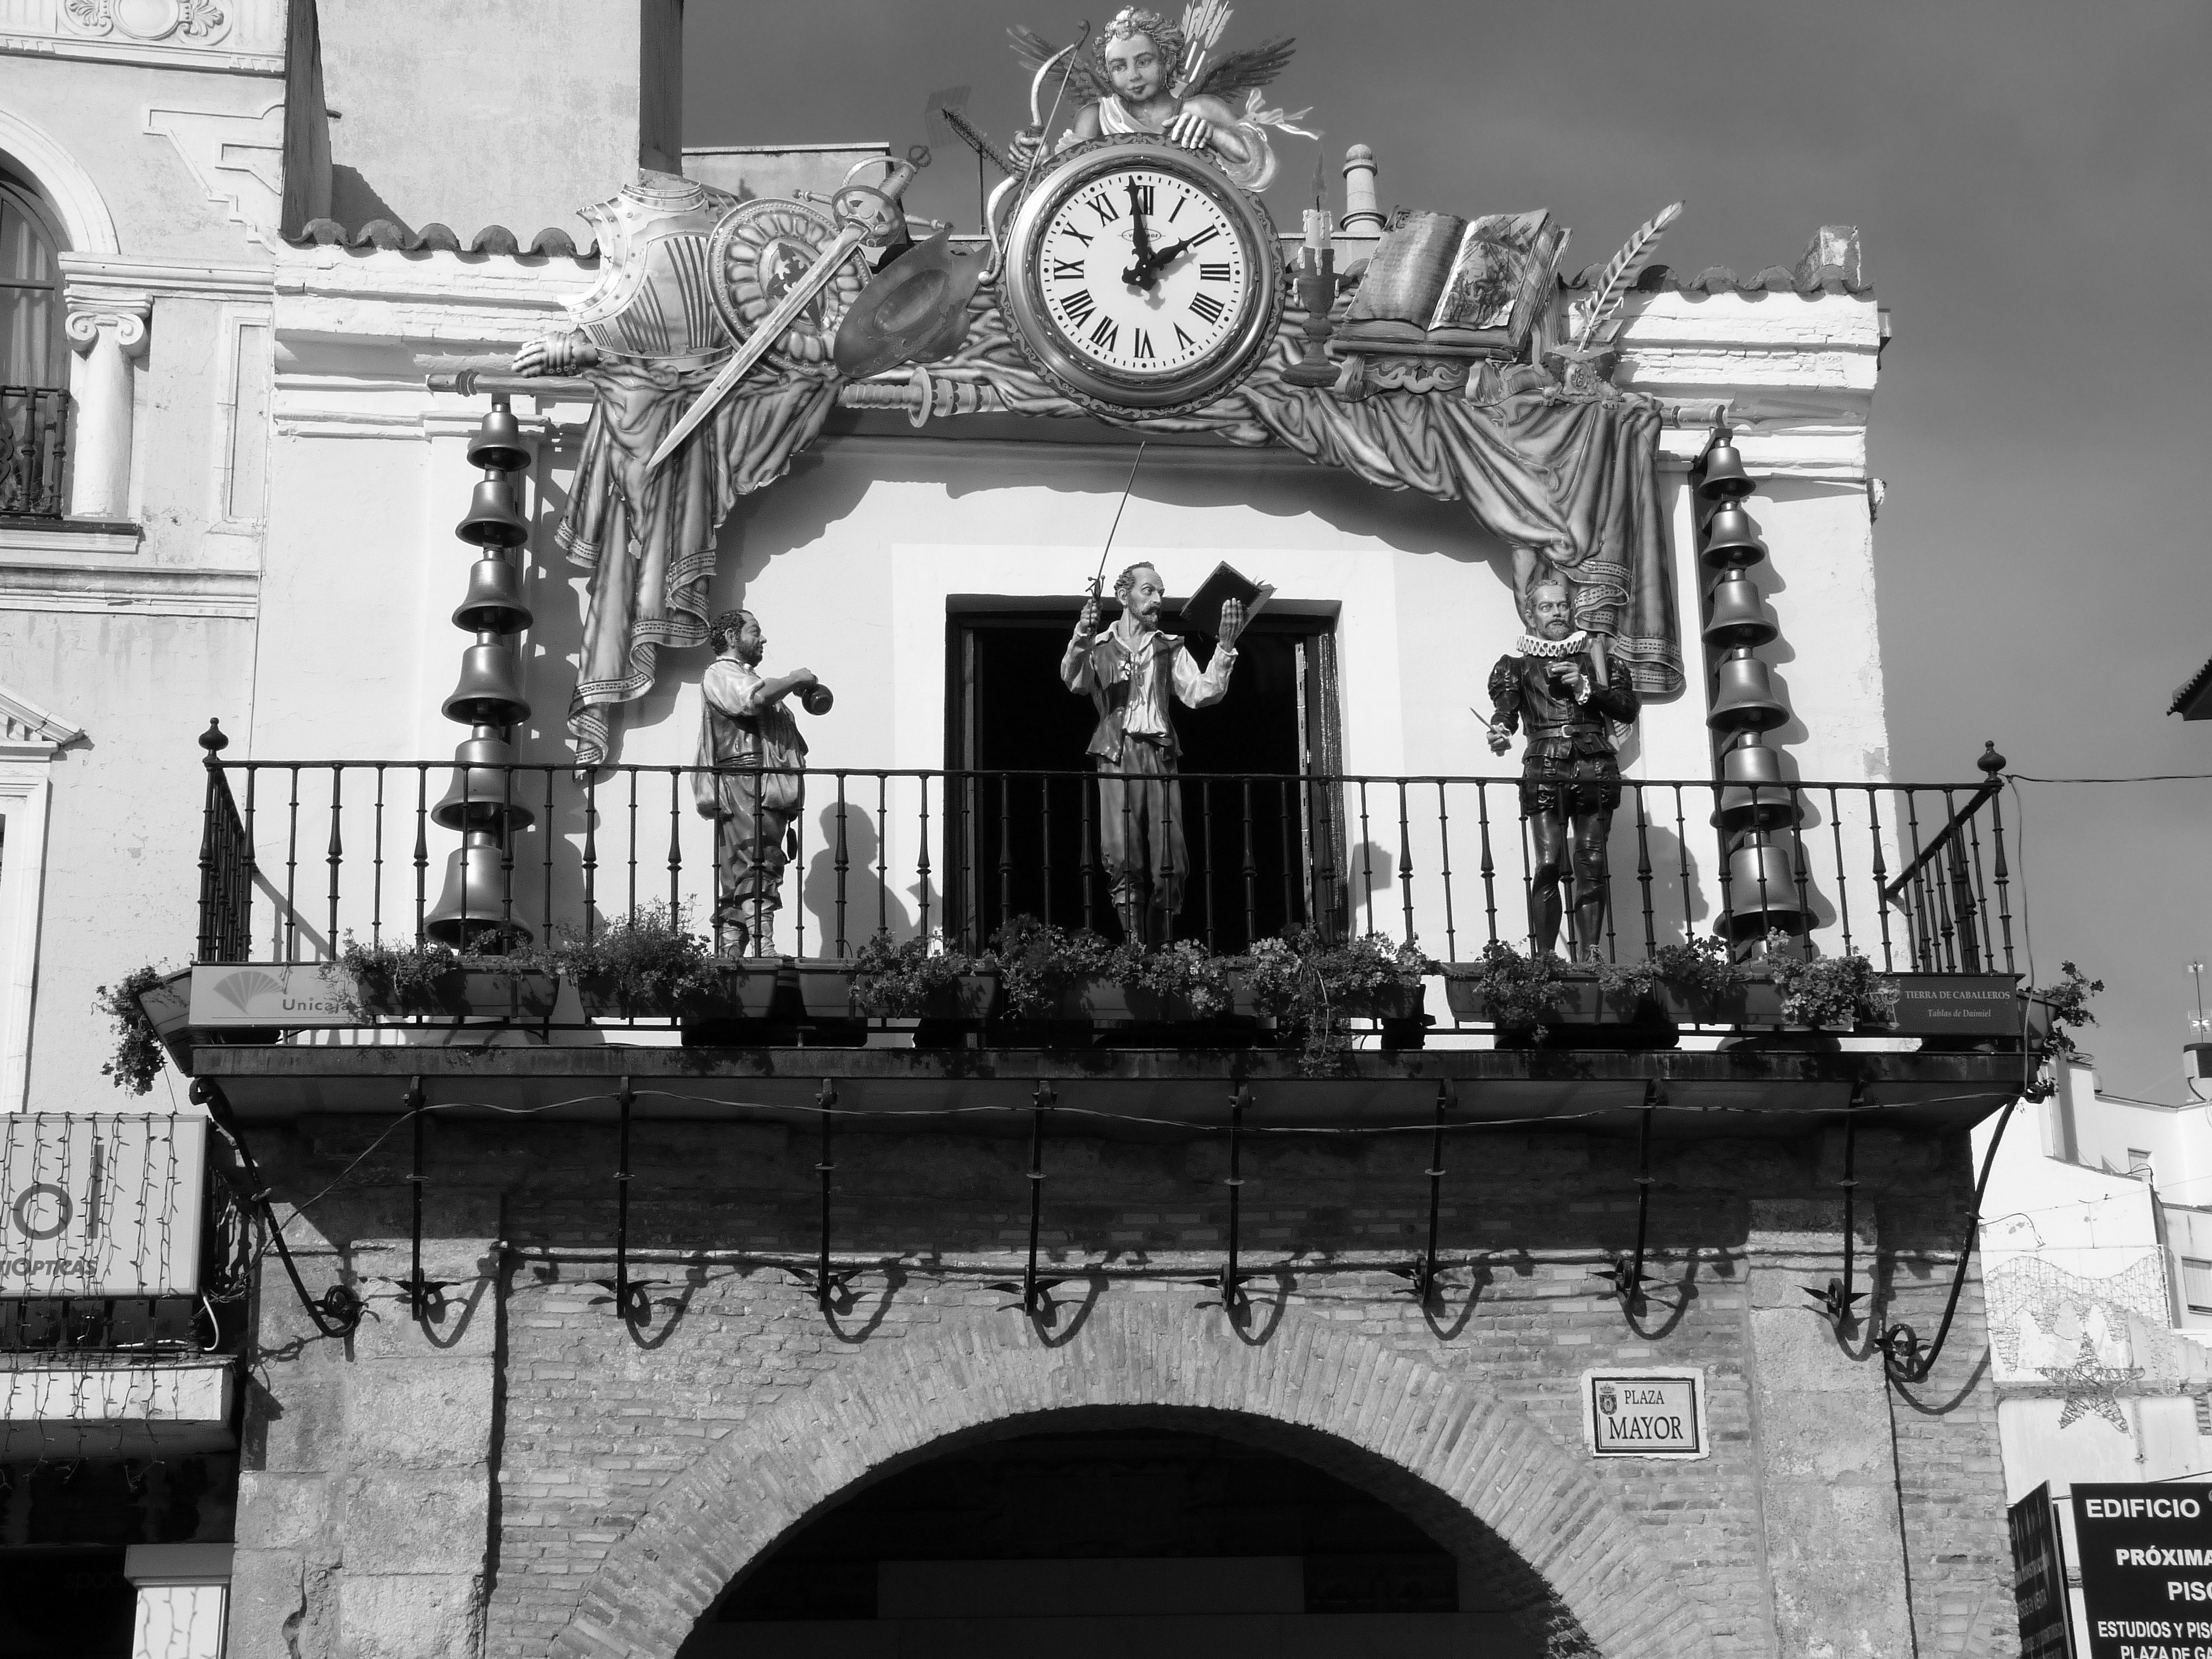
\includegraphics[width=0.8\linewidth]{./figs/clockCRbw}
		\caption{Fotografía en blanco y negro}\label{fig:fotoBW}
	\end{subfigure} 
	\caption[Ejemplo de subfiguras]{Ejemplo de inclusión de subfiguras en un mismo entorno (Fuente: J. Salido, \faCreativeCommons{} \faCreativeCommonsBy{} \faCreativeCommonsNcEu{} \faCreativeCommonsNd)}
	\label{fig:ejSubfigures}
\end{figure}

En los trabajos académicos la inclusión de imágenes y figuras que no son propiedad del autor suscitan bastante controversia, ya que con frecuencia se incumple inadvertidamente la ley vigente de propiedad intelectual. Respecto a este hecho se recomienda, tanto a estudiantes como tutores, consultar documentación informativa sobre el uso correcto de figuras en documentos académicos \cite{uclm20,unican18}. Entre las <<incorrecciones>> más habituales en los documentos académicos, se observa:
\begin{itemize}
\item \emph{Abuso del derecho de cita}. Se produce al incluir, con fines exclusivamente decorativos o ilustrativos de la explicación, una figura sujeta a derechos de uso restringido invocando el derecho de cita (incluso con correcta atribución de la obra).

\item \emph{Incorrecta atribución de la obra}. Es habitual confundir al autor de la obra con la fuente de origen de la misma. La fuente es precisa cuando se cita la obra original. Sin embargo, la licencia de muchas obras exige la atribución al autor y la inclusión de la licencia bajo la que se distribuye o hace uso de la misma (véase como ejemplo cómo se realiza una correcta atribución en las Fig.~\ref{fig:ejFigure} y \ref{fig:ejSubfigures} mencionando al autor y la licencia Creative-Commons\footnote{\url{https://creativecommons.org}} bajo la que se rige el uso de la imagen y el mecanismo de título alternativo para que dicha atribución no aparezca en el índice de figuras usando título opcional).

\item \emph{Supresión de los detalles de la licencia de uso}. Al incluir obras de terceros debemos tener presente los términos de distribución de la misma e incluirlos junto a la atribución de su legítimo autor.
\end{itemize}

La inclusión de material de \emph{dominio público}, sin restricciones de uso o con permiso, hace innecesaria la atribución al autor, pero se recomienda incluir una nota de agradecimiento.\footnote{Incluyendo un texto como: \emph{<<Por cortesía de ...>>}}

Cuando se presenta la necesidad de incluir un gráfico demasiado grande para el tamaño de la página, una opción muy apropiada es la impresión del gráfico en modo girado en una página aparte. Este efecto se consigue con el entorno \texttt{sidewaysfigure} proporcionado por el paquete \texttt{rotating}. La Fig.~\ref{fig:girada} muestra un ejemplo del entorno citado con un gráfico \textsf{PDF}.

\begin{sidewaysfigure}
	\centering
	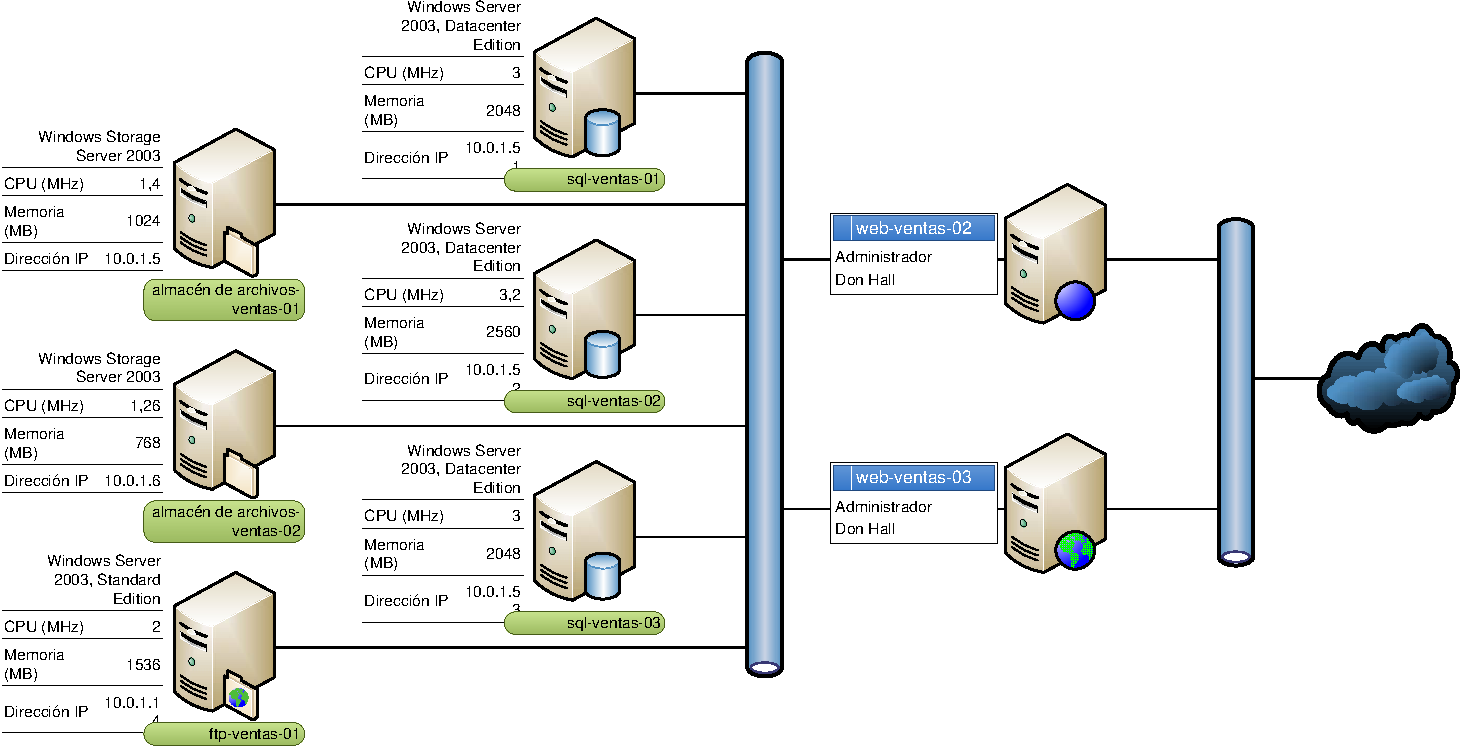
\includegraphics[width=0.98\textheight]{./figs/network} 
	\caption[Gráfico girado]{Figura vectorial con impresión girada}
	\label{fig:girada}
\end{sidewaysfigure}


\begin{landscape}
\thispagestyle{empty}
También es posible imprimir una página en formato apaisado cuando contiene una figura muy ancha. Este efecto se consigue con el paquete \texttt{pdflscape} y el entorno \texttt{landscape} proporcionado. Además, es este caso se han suprimido tanto la cabecera como el pie de página. La figura~\ref{fig:apaisada} se muestra apaisada a modo de ejemplo.

\begin{figure}[H]
	\centering
	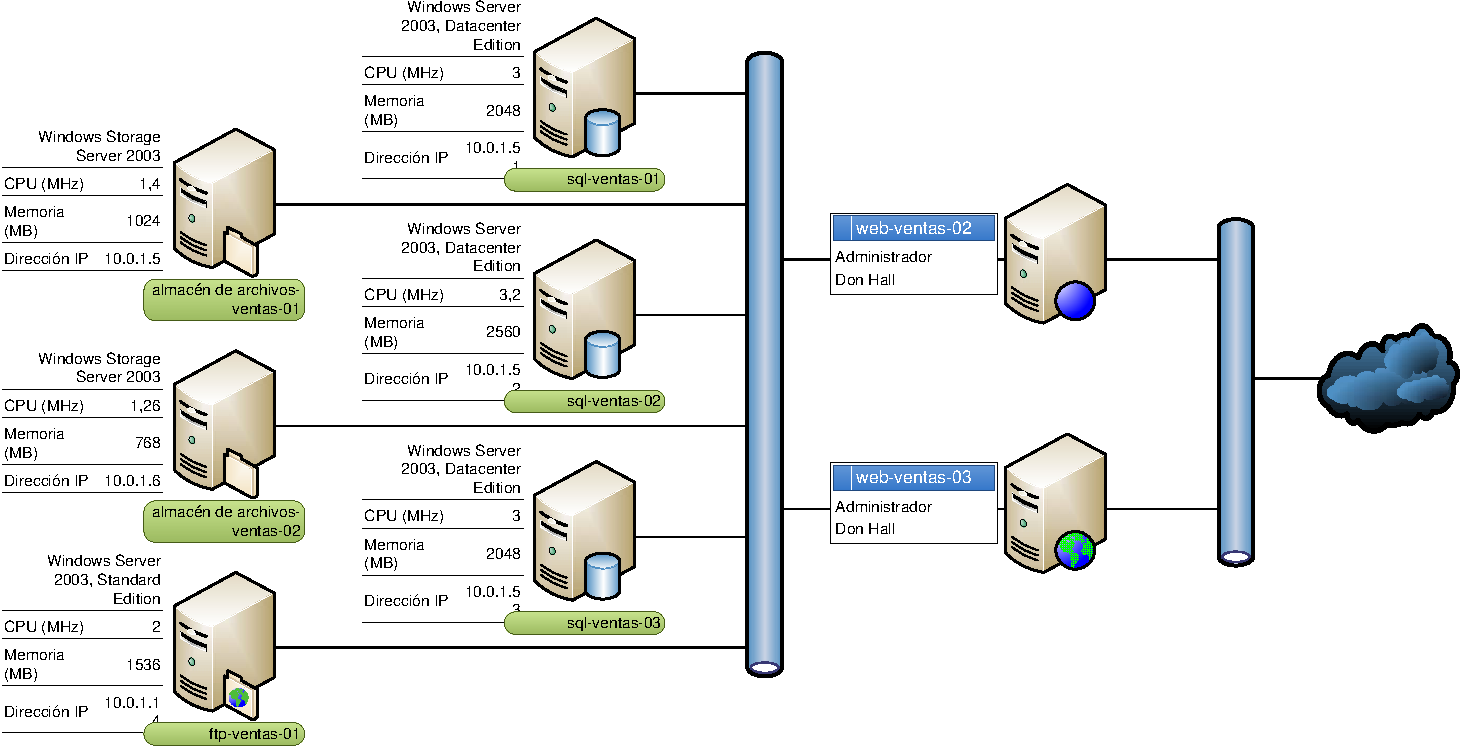
\includegraphics[width=\linewidth]{./figs/network} 
	\caption[Gráfico apaisado]{Figura vectorial con vista en página apaisada}
	\label{fig:apaisada}
\end{figure}
\end{landscape}


\section{Algoritmos y listados de código fuente}
En los textos científicos relacionados con las 
TIC\footnote{Por supuesto, en un TFG (Trabajo Fin de Grado) o tesis 
de un centro superior de Informática.} (Tecnologías de la Información y 
Comunicaciones) suelen aparecer porciones de código en los que se explica 
alguna función o característica relevante del trabajo que se expone. Muchas 
veces lo que se quiere ilustrar es un algoritmo o método con el que se resuelve un problema abstrayéndose del lenguaje de implementación. El paquete \texttt{algorithm2e} proporciona un entorno \texttt{algorithm} para la impresión apropiada de algoritmos, tratándolos como objetos flotantes y con mucha flexibilidad de personalización, como se observa en el algoritmo~\ref{alg:como} del ejemplo.


% Ejemplo:
% ============
\IncMargin{1em}
\begin{algorithm}
\SetKwInOut{Input}{Datos}\SetKwInOut{Output}{Resultado}
\LinesNumbered
\SetAlgoLined

\Input{este texto} 
%\KwIn{este texto}
\Output{como escribir algoritmos con \LaTeX2e}
%\KwOut{como escribir algoritmos con \LaTeX2e}

inicialización\;
\While{no es el fin del documento}{
	leer actual\;
	\eIf{comprendido}{
		ir a la siguiente sección\;
		la sección actual es esta\;
	}{
		ir al principio de la sección actual\;
	}
}

% Aunque el captión aparece abajo siempre se pone arriba como en tablas y listados
\caption{Cómo escribir algoritmos}\label{alg:como}
\end{algorithm}\DecMargin{1em}








\newpage % Añadido para visualizar los listados completos en una página.
La inclusión de porciones de código fuente se puede formatear de modo sencillo en \LaTeX{} mediante el uso del paquete \texttt{listings}. A continuación, se muestran varios ejemplos de porciones de código correspondientes a distintos lenguajes de programación.


% Ejemplo: Listado Java
% ============
% Los entornos lstlisting se pueden tratar tambión como elementos flotantes mediante la opción 'float=hbt', donde se indica la ubicación del elemento.
\begin{lstlisting}[language=Java,caption={[Código fuente en Java]Ejemplo de código fuente en lenguaje Java},label=lst:java]
// @author www.javadb.com
public class Main {    
// Este método convierte un String a un vector de bytes

public void convertStringToByteArray() {

String stringToConvert = "This String is 15";      
	byte[] theByteArray = stringToConvert.getBytes();        
	System.out.println(theByteArray.length);        
}

public static void main(String[] args) {
	new Main().convertStringToByteArray();
}
}
\end{lstlisting}


\begin{lstlisting}[style=ruled,language=C,caption={Ejemplo de código fuente en lenguaje C},label=lst:codC]
// Este código se ha incluido tal cual está en el fichero \LaTeX{}
#include <stdio.h>

int main(int argc, char* argv[]) {
	puts("¡Hola mundo!");
}
\end{lstlisting}


\begin{lstlisting}[style=ruled,language=Matlab,caption={Ejemplo de script en Matlab},label=lst:matlab]
function f = fibonacci(n)
% FIBONACCI  Fibonacci sequence
% f = FIBONACCI(n) generates the first n Fibonacci numbers.
%   Copyright 2014 Cleve Moler
% 	Copyright 2014 The MathWorks, Inc.

	f = zeros(n,1); 
	f(1) = 1;
	f(2) = 2;
	for k = 3:n
		f(k) = f(k-1) + f(k-2);
end
\end{lstlisting}



\section{Menús, paths y teclas con el paquete \texttt{menukeys}}
Cada vez es más usual que los trabajos en ingeniería exijan el uso de 
software. Para poder especificar de modo elegante el uso de menús, pulsaciones de teclas y directorios, se recomienda el uso del paquete 
\texttt{menukeys}.\footnote{\url{https://osl.ugr.es/CTAN/macros/latex/contrib/menukeys/menukeys.pdf}}
 \index{CTAN} Este paquete nos permite especificar el acceso a un menú, por 
ejemplo:

\noindent \menu{Herramientas:Órdenes:PDFLaTeX}

\noindent También un conjunto de teclas. Por ejemplo:
\keys{\ctrl + \shift + T}

\noindent O un directorio:
\directory{C:/user/LaTeX/Ejemplos}

\noindent Aunque este paquete permite muchas opciones de configuración de los estilos aplicados, esto no es necesario para obtener unos resultados muy elegantes.










 % Apéndice A (opcionales)

%END_FOLD
%--- (FIN DOCUMENTO)
\end{document}